\section{Predicción de los Precios del Cemento y del Ladrillo Común con Seasonal Autoregressive Integrated Moving Average with Exogenous Variables (SARIMAX)}
\vspace{0.3cm}
\justify
En esta sección se presentan los resultados de la aplicación del modelo SARIMAX (\textit{Seasonal AutoRegressive Integrated Moving Average with eXogenous inputs}) a la predicción de los precios de dos materiales de construcción: el cemento y el ladrillo común. El SARIMAX, implementado con \texttt{statsmodels}, ofrece un marco interpretable y con supuestos explícitos para la modelación de series temporales con componentes estacionales y variables exógenas. Para ambos materiales, se utilizaron como variables exógenas el nivel promedio mensual del río Paraguay (\texttt{Nivel\_Rio}), obtenido de las predicciones del modelo LSTM descrito en la sección anterior, y una variable binaria de cuarentena (\texttt{Cuarentena}) que captura el efecto de la pandemia de COVID-19. Los resultados abarcan el análisis exploratorio de cada serie, la selección y evaluación de cada modelo, y la generación de pronósticos a 24 meses bajo escenarios con y sin efecto pandémico.

% ============================================================
\subsection{Predicción del Precio del Cemento}
\vspace{0.3cm}
\justify
Con la proyección del nivel del río disponible, el siguiente paso fue modelar directamente el precio del cemento. El SARIMAX ofrece un marco interpretable y con supuestos explícitos; los resultados que se presentan a continuación abarcan el análisis exploratorio de la serie, la evaluación del modelo y la generación de pronósticos.

\subsubsection{Serie Histórica y Análisis Exploratorio}

\justify
La serie histórica empleada abarca registros mensuales del precio del cemento en Guaraníes (Gs.) desde enero de 2014 hasta julio de 2025, totalizando 139 observaciones. La variable endógena es el precio del cemento (\texttt{Precio\_Cemento}), mientras que las variables exógenas incorporadas son el nivel promedio mensual del río Paraguay (\texttt{Nivel\_Rio}), obtenido a partir de las predicciones del modelo LSTM descrito en la sección anterior, y una variable binaria de cuarentena (\texttt{Cuarentena}) que captura el efecto de la pandemia de COVID-19. Los estadísticos descriptivos de la serie son: precio mínimo de Gs.~48.000, precio máximo de Gs.~76.036, precio promedio de Gs.~53.872 y desviación estándar de Gs.~7.460.

\begin{figure}[ht]
    \centering
    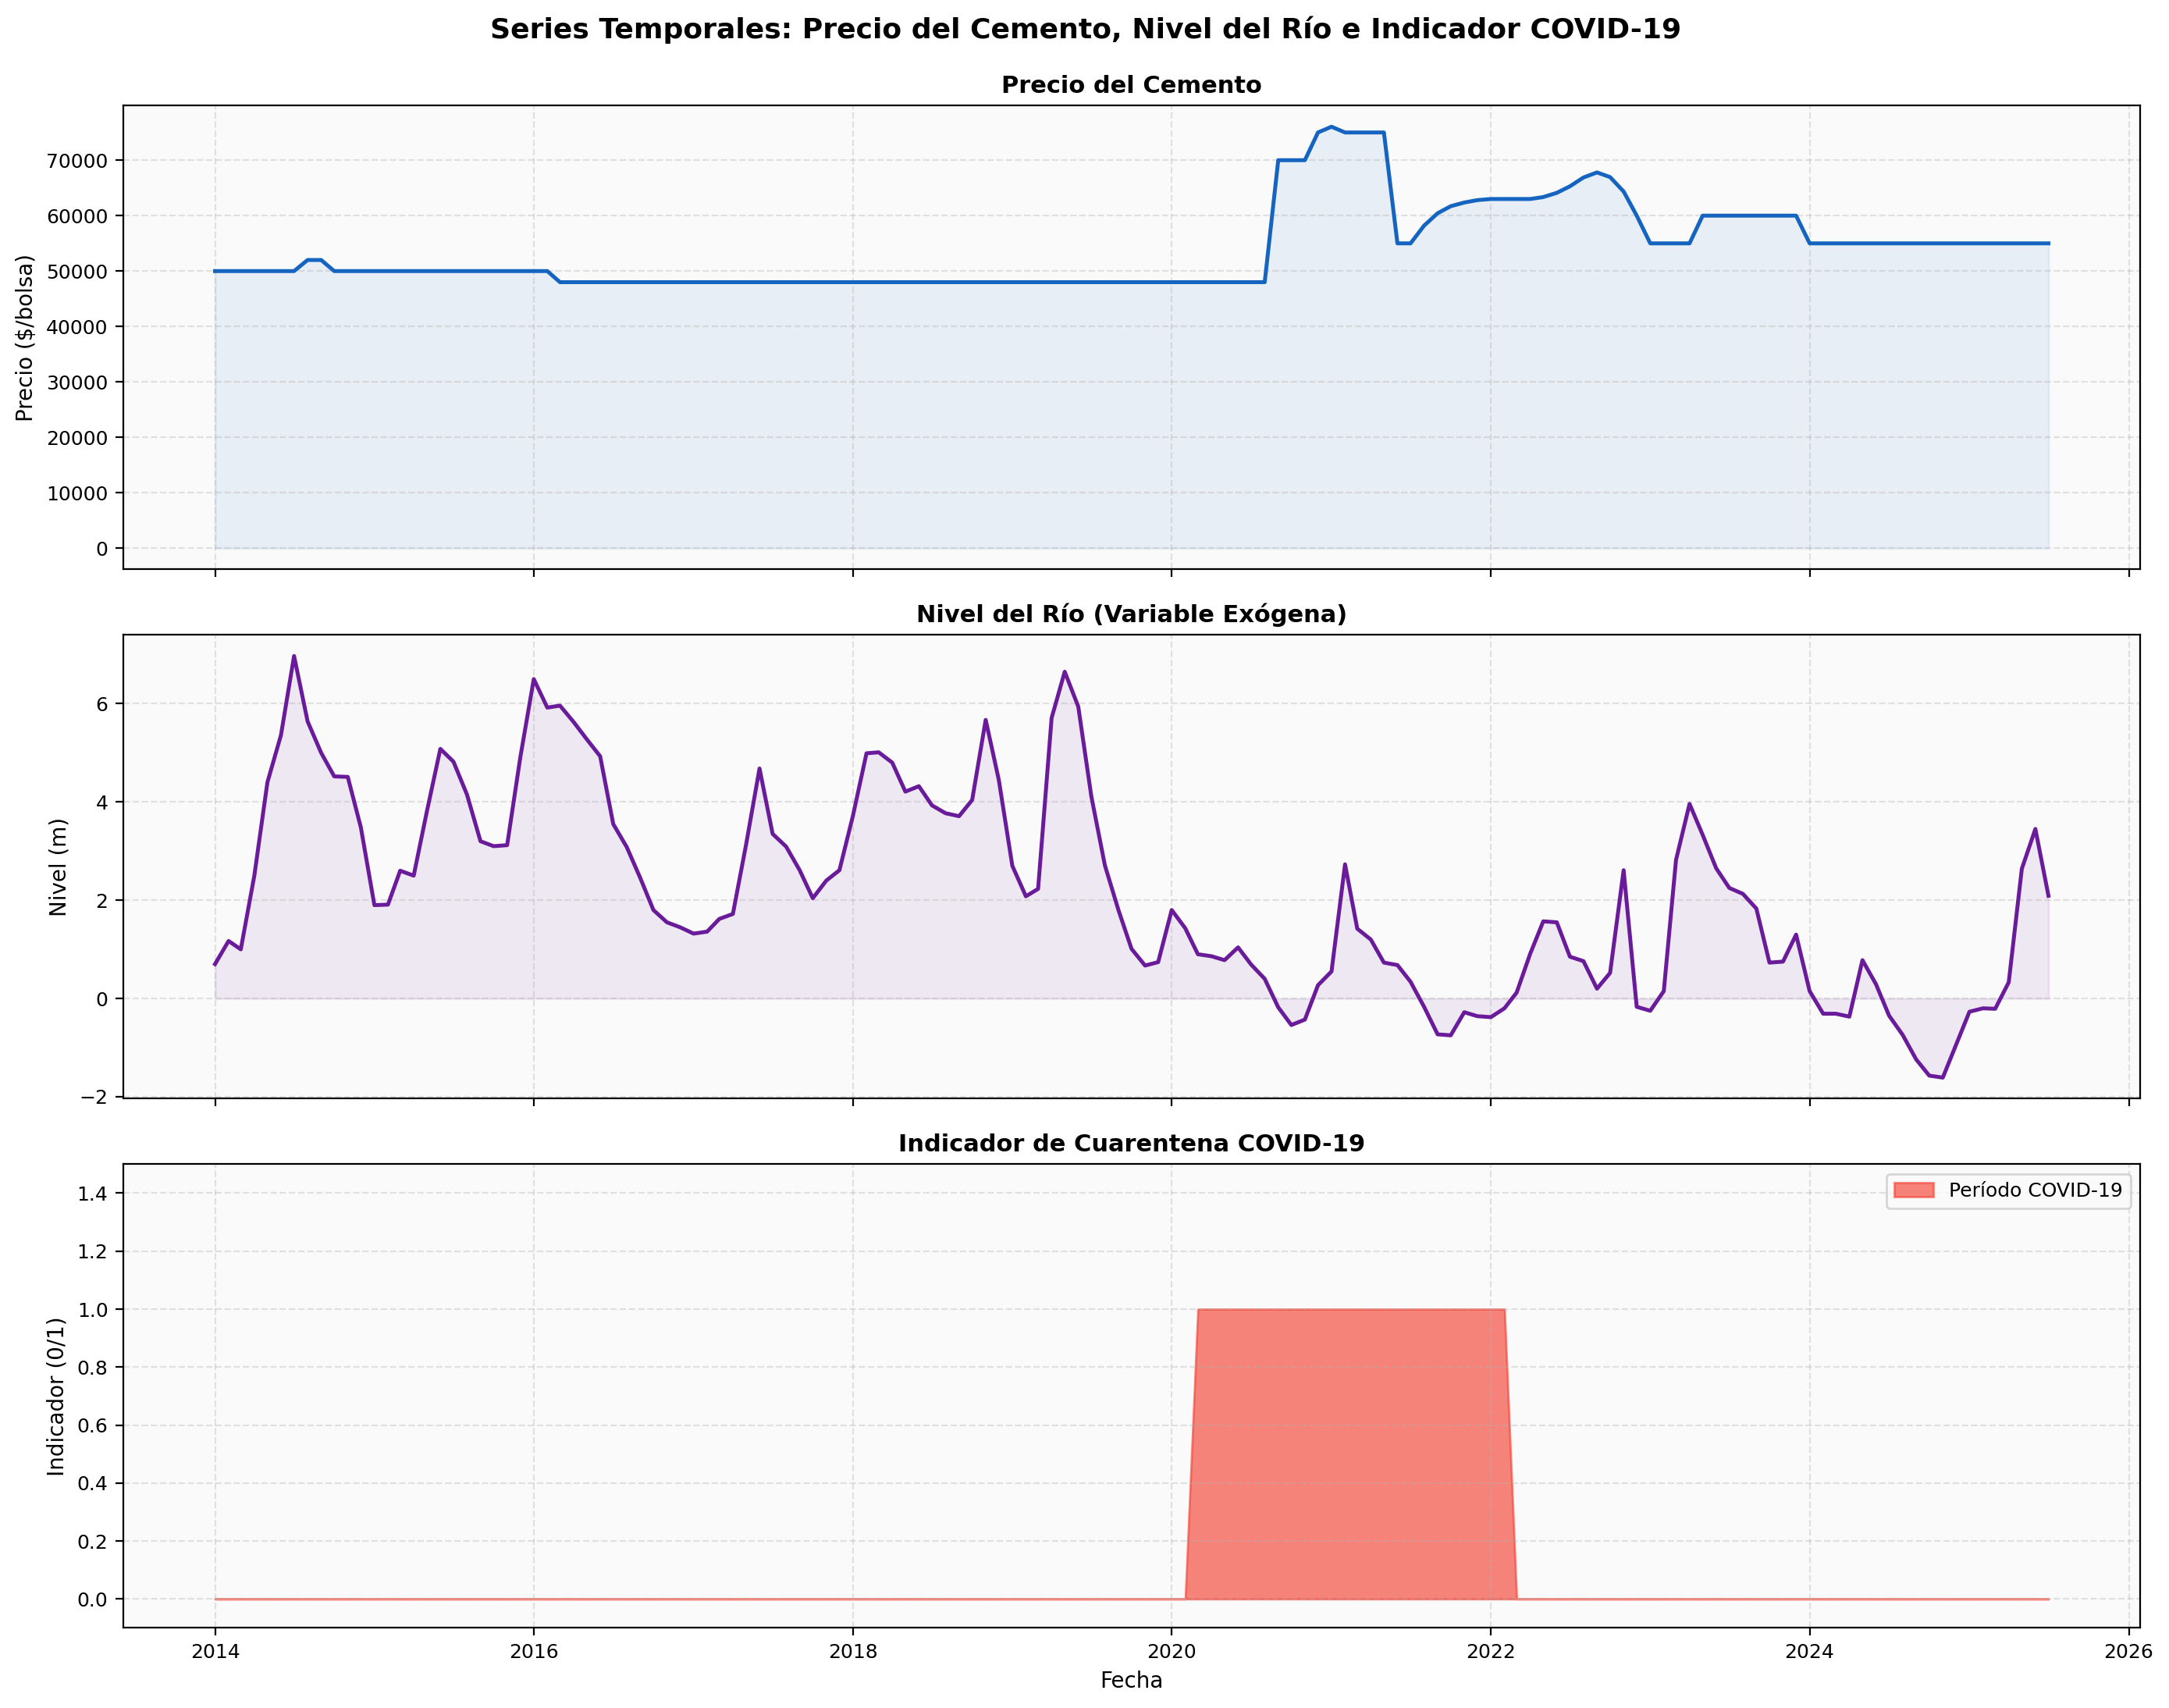
\includegraphics[width=\textwidth]{predicciones/prediccion_sarimax_cemento/graficos/01_series_temporales.png}
    \caption{Series temporales del precio mensual del cemento (Gs.) y del nivel del río Paraguay (m), período 2014--2025.}
    \label{fig:sarimax_series}
\end{figure}

\justify
La Figura \ref{fig:sarimax_series} muestra la evolución conjunta del precio del cemento y del nivel del río Paraguay. Se aprecia una tendencia ascendente sostenida en el precio del cemento a lo largo del período analizado, con una aceleración marcada a partir de 2020 que coincide con el período de pandemia y las disrupciones en la cadena de suministros. El nivel del río, por su parte, presenta la variabilidad estacional interanual característica, con ciclos de crecida y estiaje que constituyen la variable exógena hidrológica del modelo.

\begin{figure}[ht]
    \centering
    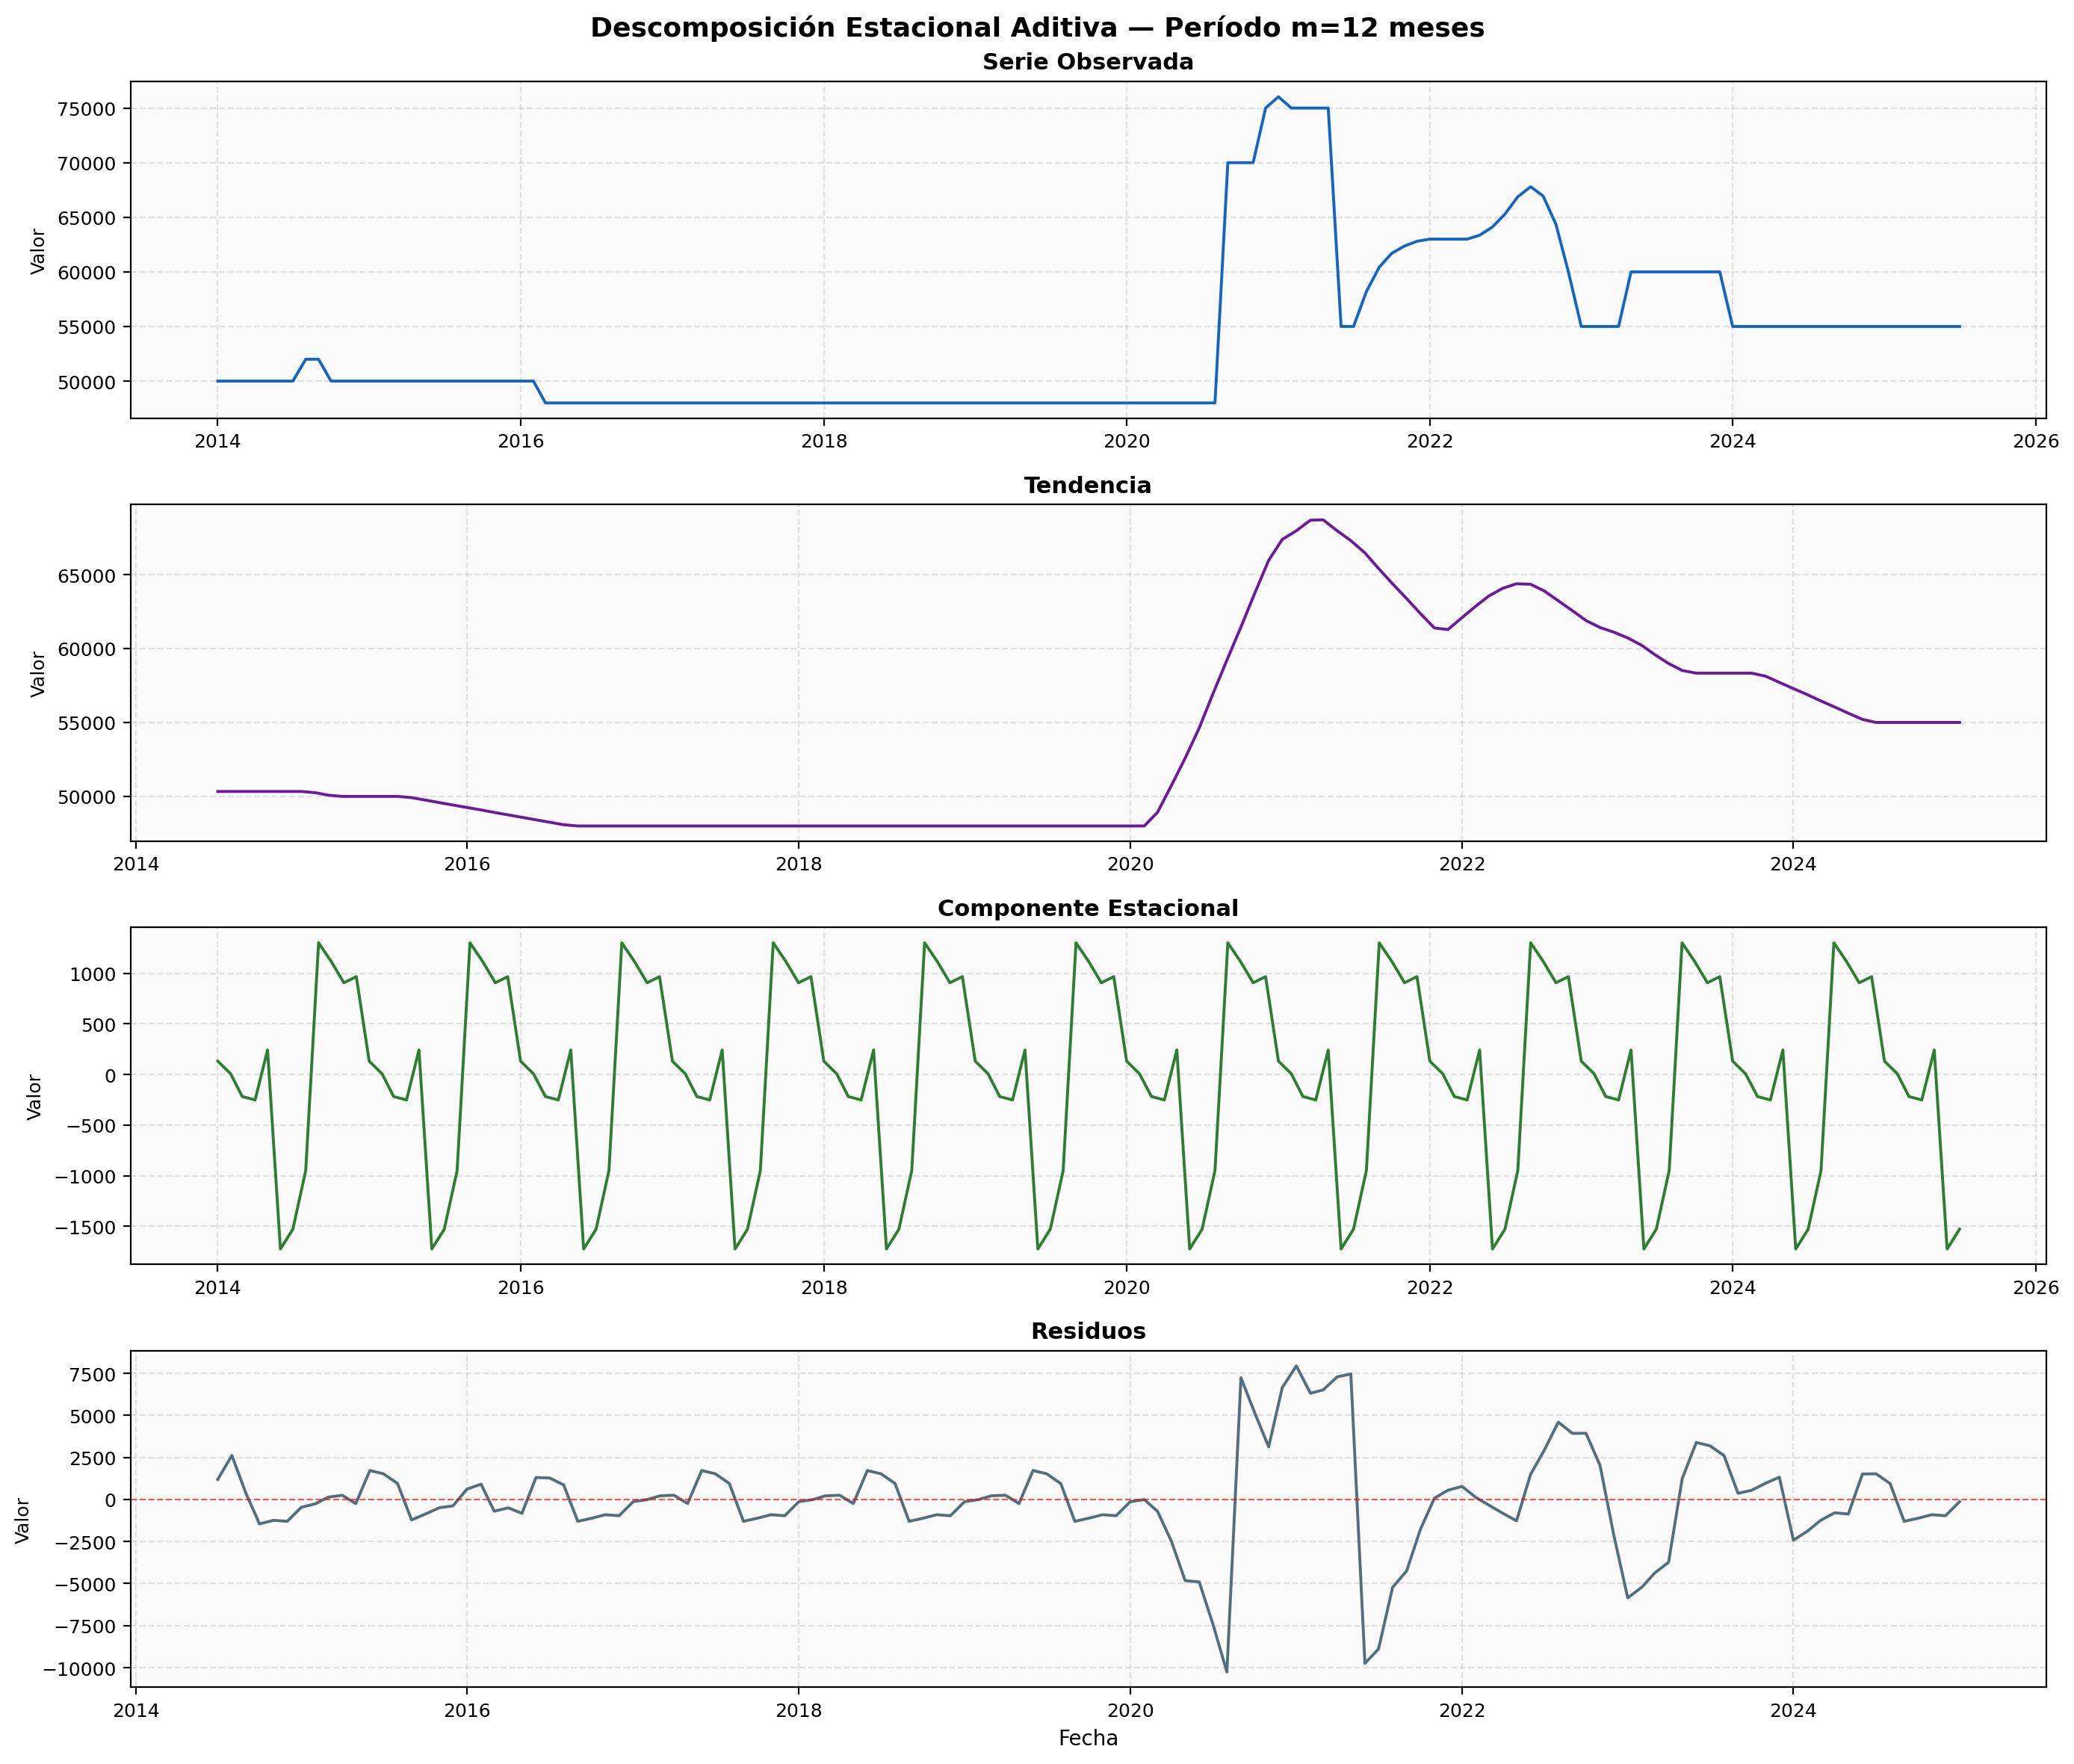
\includegraphics[width=\textwidth]{predicciones/prediccion_sarimax_cemento/graficos/02_descomposicion_estacional.png}
    \caption{Descomposición estacional de la serie de precio del cemento: tendencia, estacionalidad y componente residual.}
    \label{fig:sarimax_descomposicion}
\end{figure}

\justify
La Figura \ref{fig:sarimax_descomposicion} presenta la descomposición clásica de la serie en sus componentes de tendencia, estacionalidad y residuo. La componente de tendencia confirma el crecimiento sostenido del precio, en particular el salto registrado entre 2020 y 2022. La componente estacional revela patrones de amplitud moderada con período anual, mientras que los residuos no evidencian estructura sistemática evidente, lo que sugiere la adecuación de la descomposición.

\begin{figure}[ht]
    \centering
    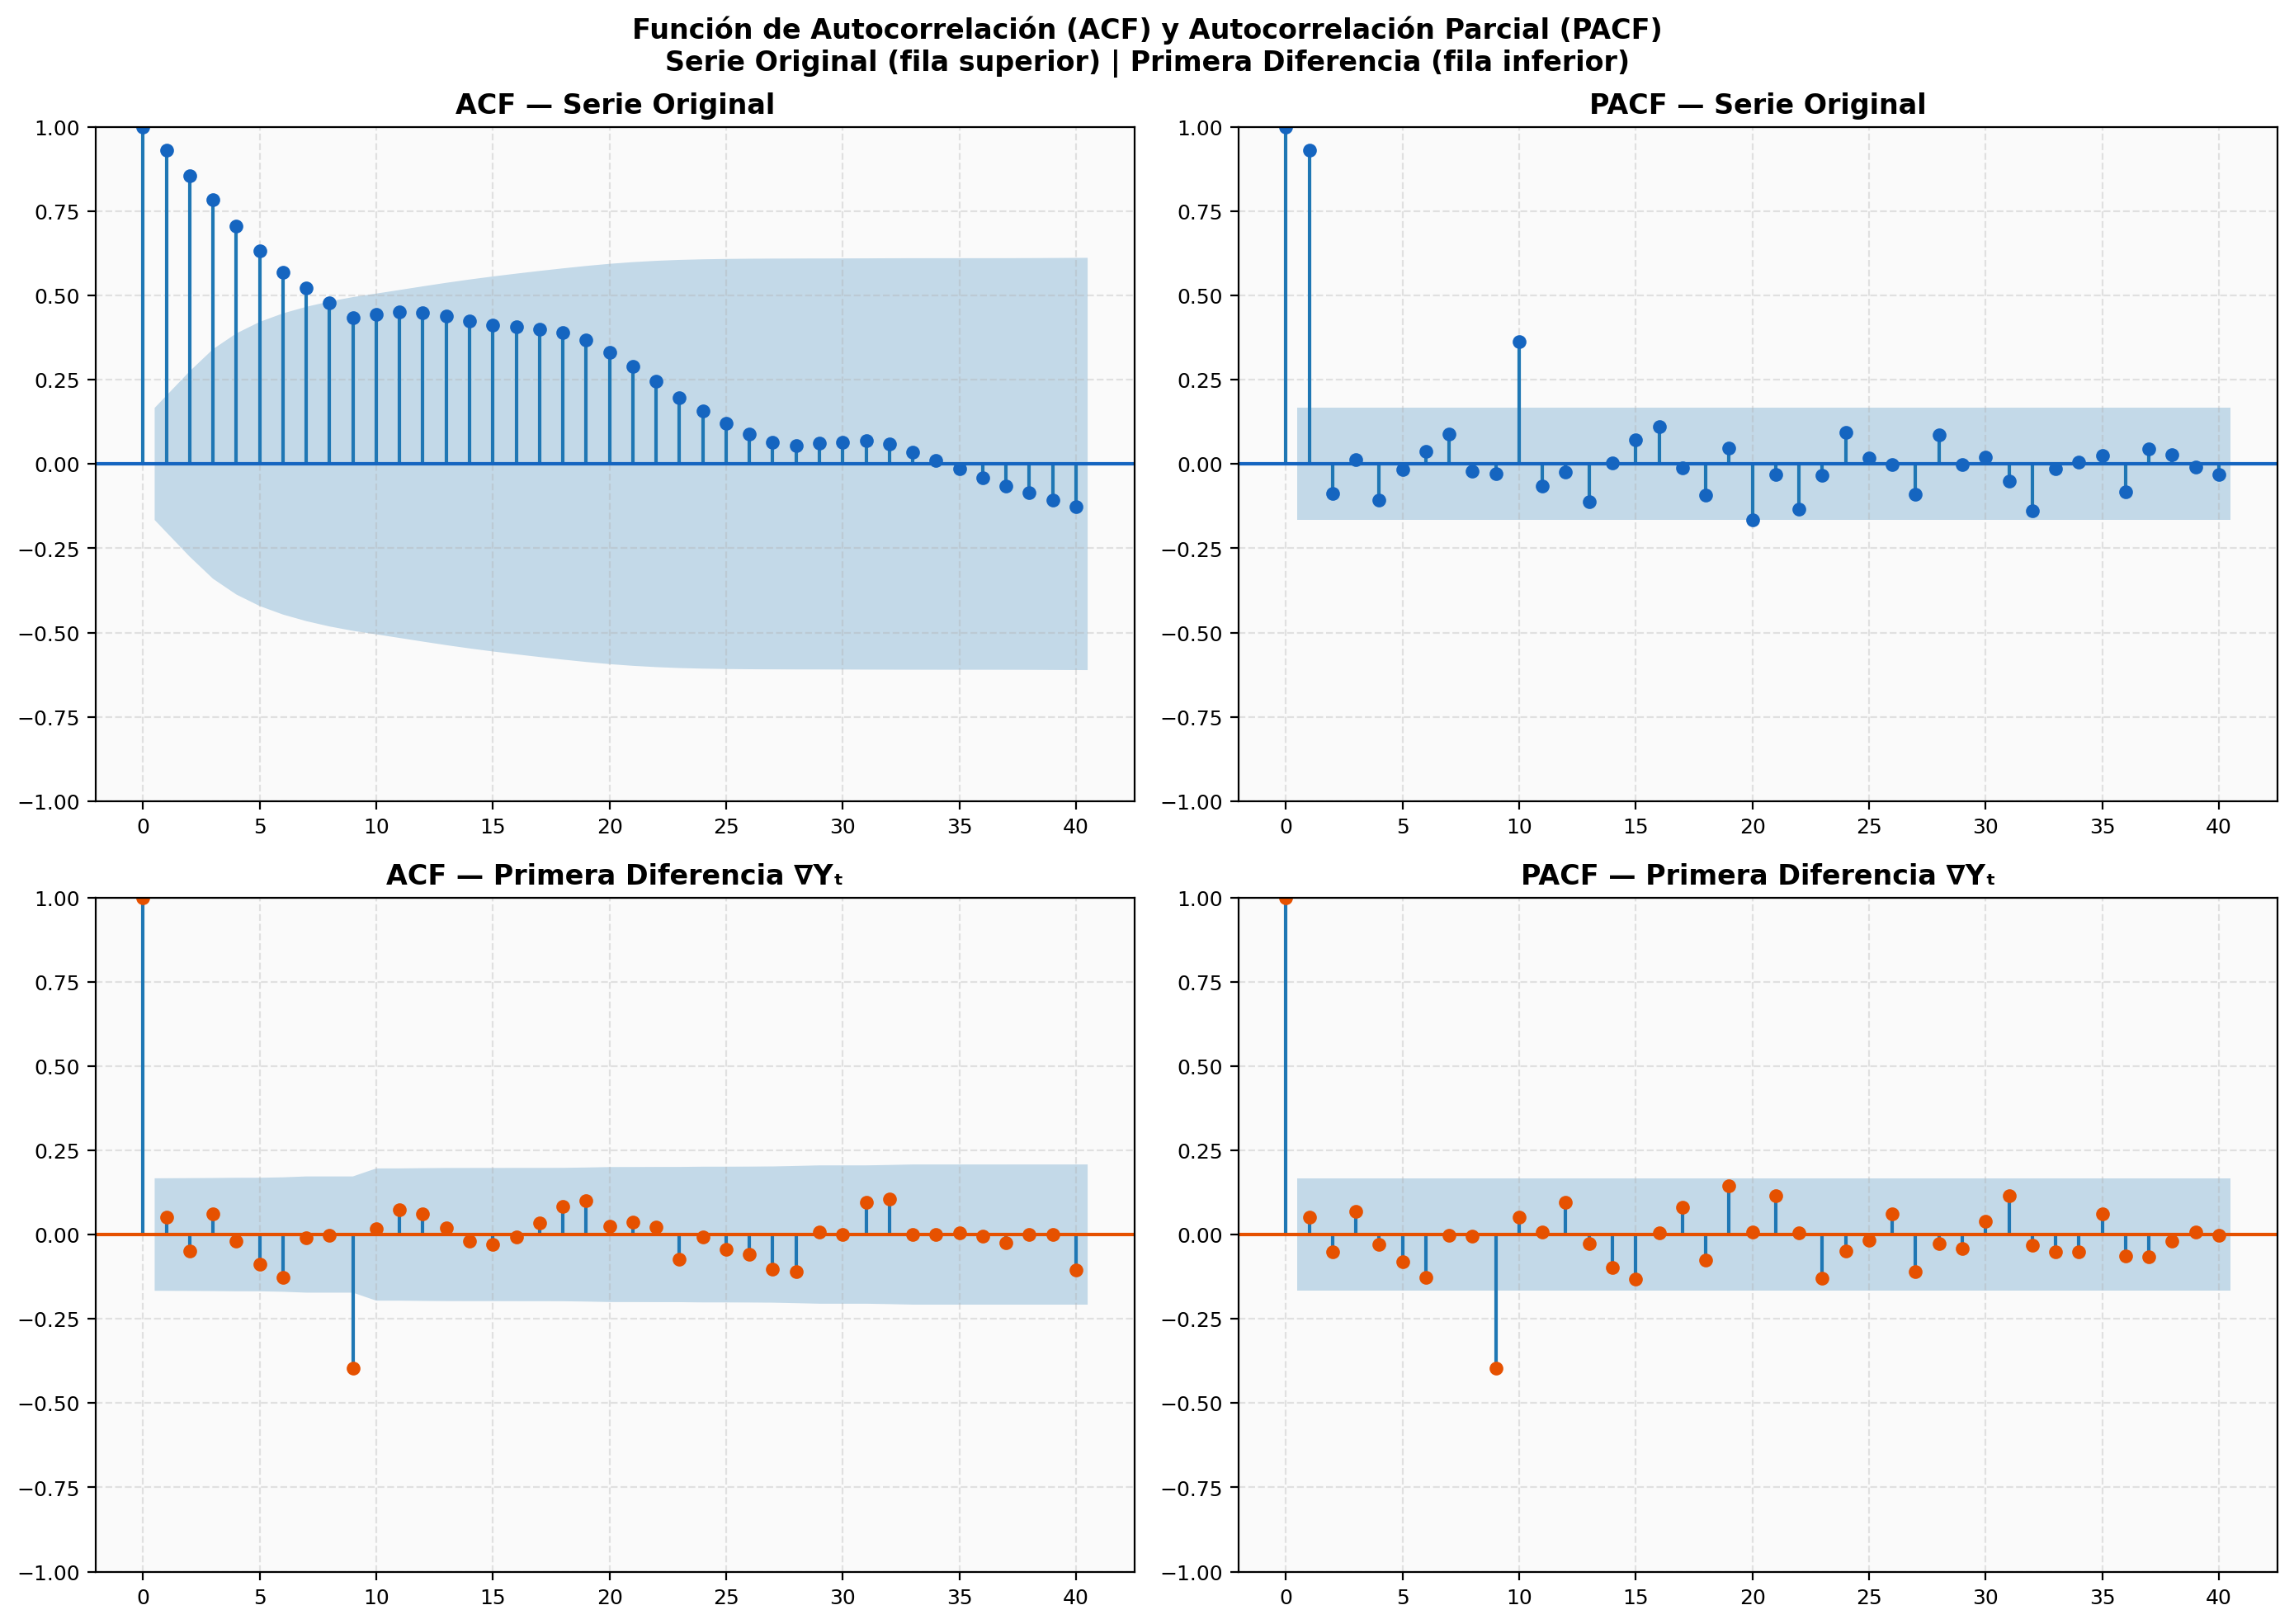
\includegraphics[width=\textwidth]{predicciones/prediccion_sarimax_cemento/graficos/03_acf_pacf.png}
    \caption{Funciones de autocorrelación (ACF) y autocorrelación parcial (PACF) de la serie del precio del cemento en niveles y en primeras diferencias.}
    \label{fig:sarimax_acf_pacf}
\end{figure}

\justify
La Figura \ref{fig:sarimax_acf_pacf} muestra las funciones ACF y PACF de la serie original y de su primera diferencia. La serie en niveles presenta una ACF con decaimiento lento, característico de procesos no estacionarios integrados. Tras aplicar la primera diferencia, la ACF decae abruptamente hacia cero a partir del primer rezago, lo que indica que la serie diferenciada es estacionaria. Este diagnóstico justifica el orden de integración $d=1$ adoptado en el modelo SARIMAX.

\begin{figure}[ht]
    \centering
    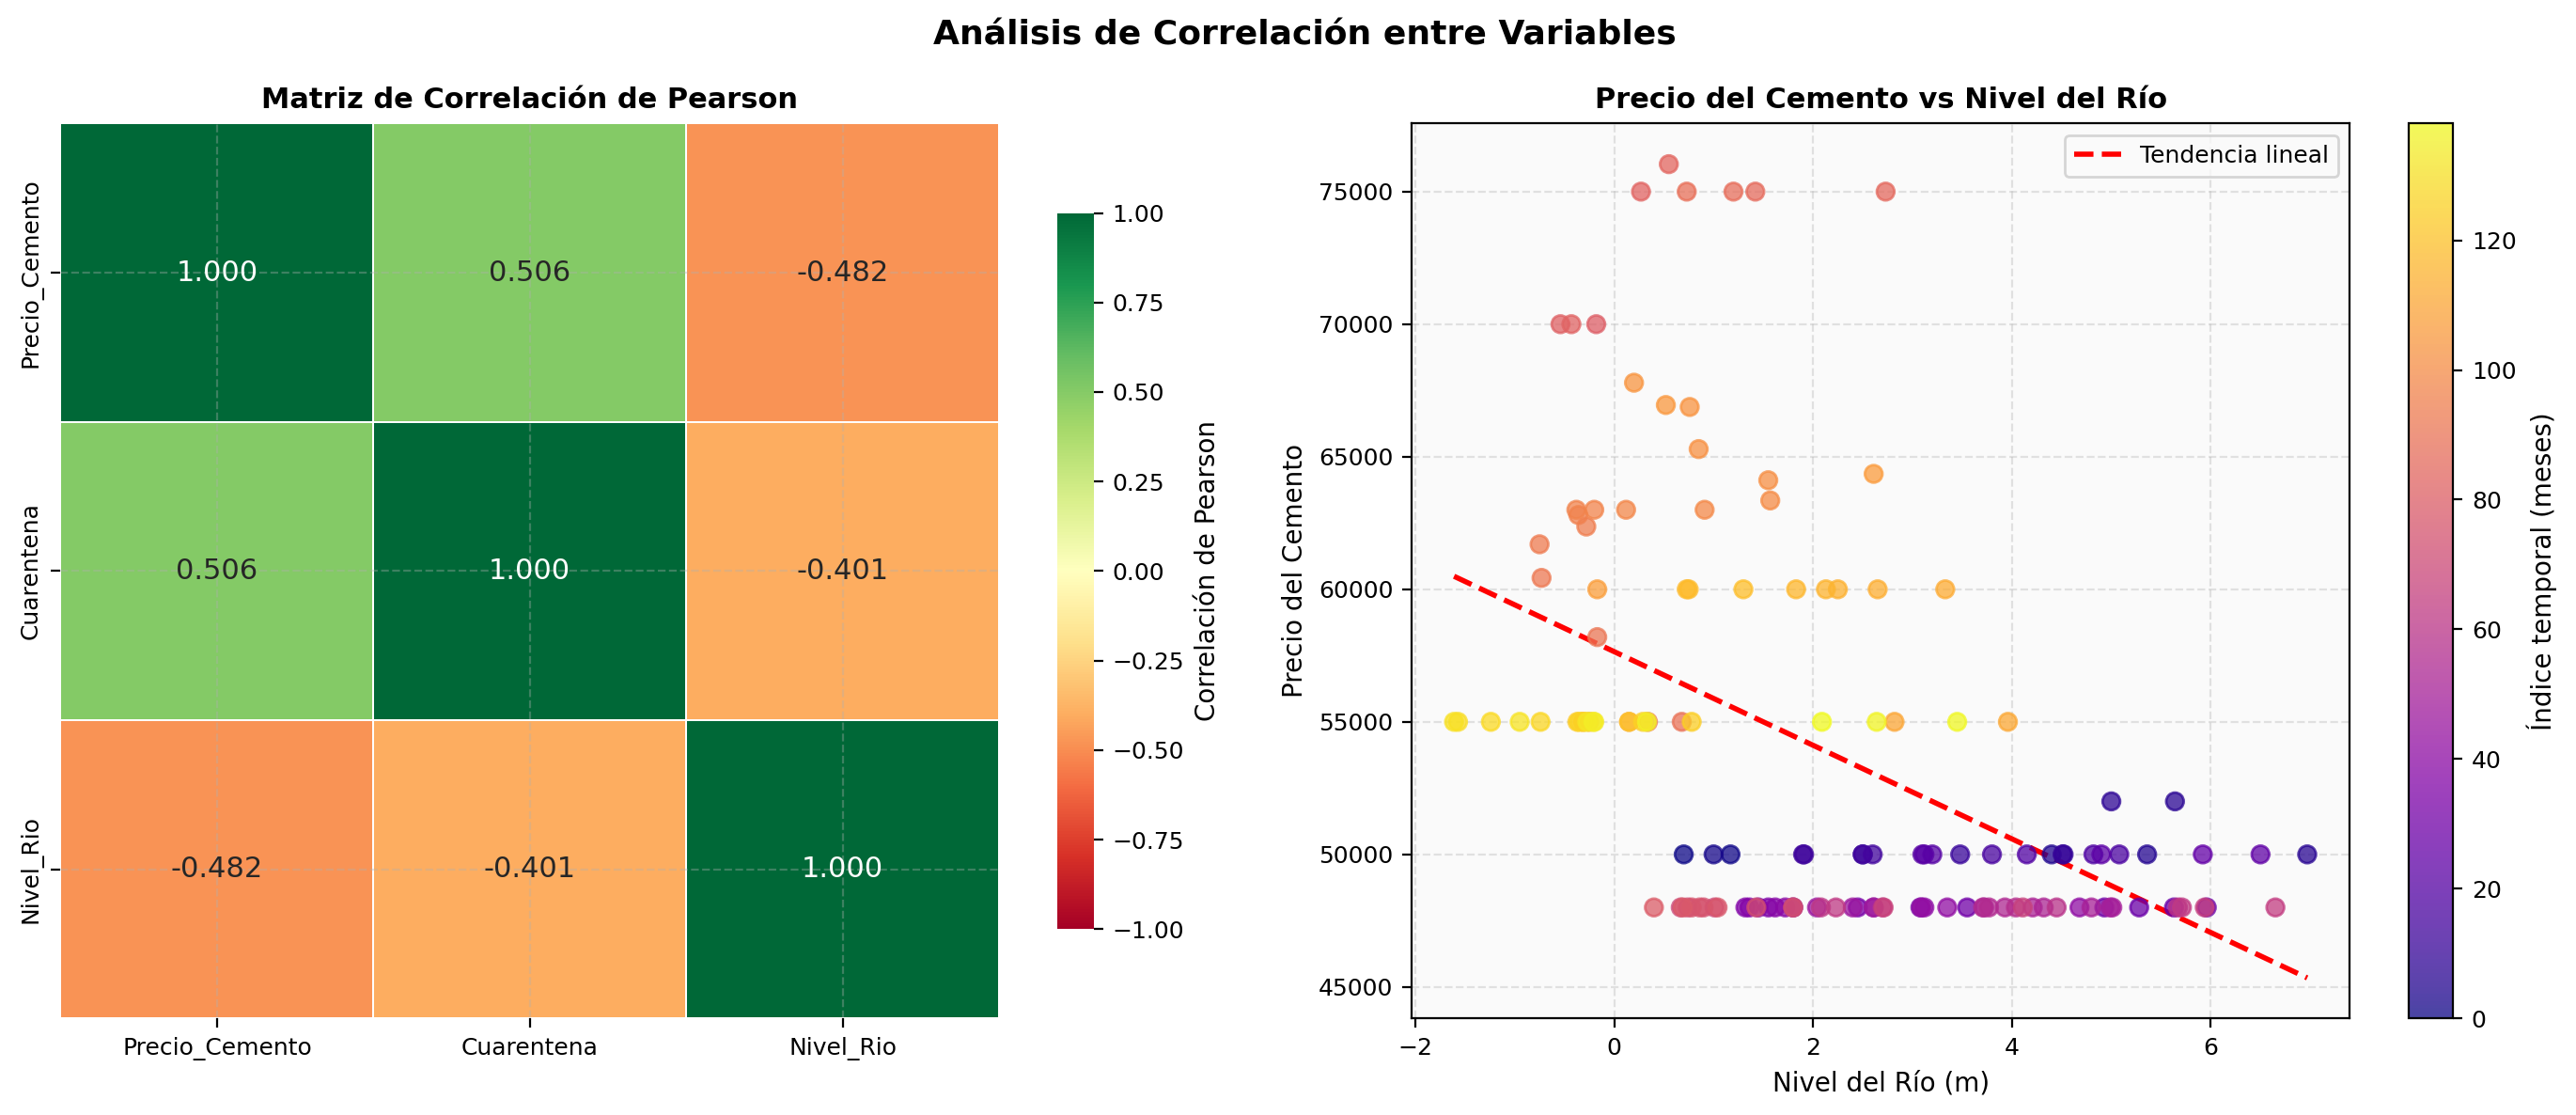
\includegraphics[width=0.8\textwidth]{predicciones/prediccion_sarimax_cemento/graficos/04_correlacion.png}
    \caption{Matriz de correlación entre el precio del cemento, el nivel del río Paraguay y la variable de cuarentena.}
    \label{fig:sarimax_correlacion}
\end{figure}

\justify
La Figura \ref{fig:sarimax_correlacion} presenta la matriz de correlación entre las variables del modelo. La correlación entre el precio del cemento y el nivel del río Paraguay es de magnitud moderada y negativa, coherente con la hipótesis de que los períodos de crecida dificultan la logística de abastecimiento y presionan al alza los costos. La variable de cuarentena muestra correlación positiva con el precio, capturando el efecto inflacionario del período pandémico.

\begin{figure}[ht]
    \centering
    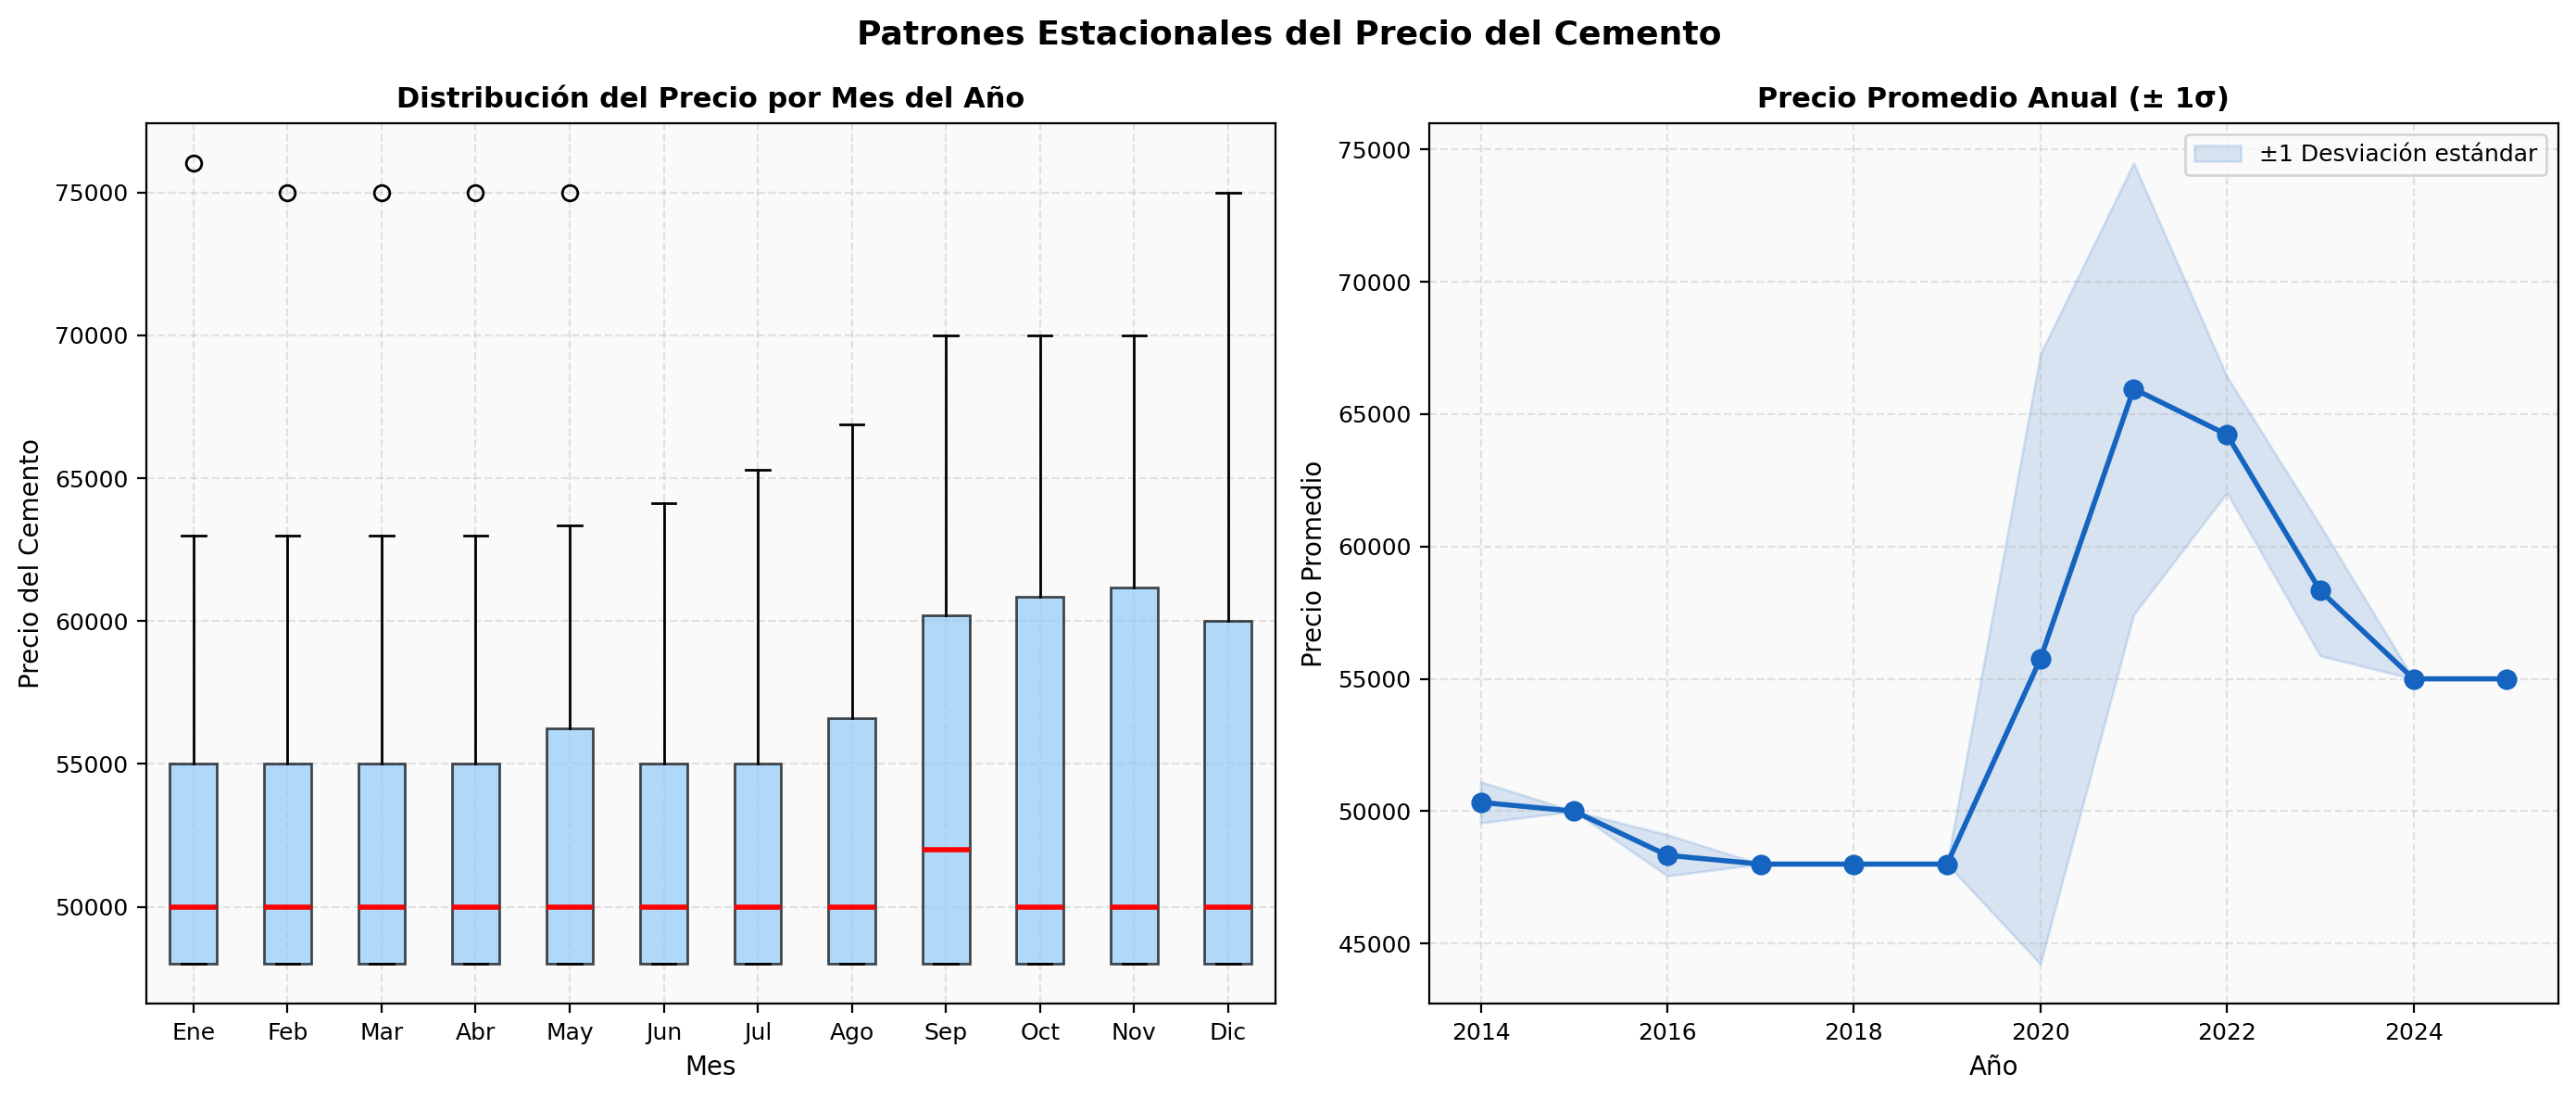
\includegraphics[width=\textwidth]{predicciones/prediccion_sarimax_cemento/graficos/05_patron_estacional.png}
    \caption{Patrón estacional del precio mensual del cemento a lo largo del año.}
    \label{fig:sarimax_estacional}
\end{figure}

\justify
La Figura \ref{fig:sarimax_estacional} ilustra el patrón estacional del precio del cemento a lo largo del ciclo anual. Se observa que los precios tienden a ser ligeramente superiores en los meses de mayor actividad de la construcción (primer y cuarto trimestre), mientras que en los meses de lluvia intensa y posibles interrupciones logísticas se registran variaciones de menor amplitud, aunque dentro de un rango de fluctuación contenido.

\subsubsection{Modelo SARIMAX: Selección y Parámetros}

\justify
La selección del orden óptimo del modelo SARIMAX se realizó mediante una búsqueda exhaustiva sobre el espacio de parámetros $(p, d, q) \times (P, D, Q)_{12}$, minimizando el Criterio de Información de Akaike (AIC). El modelo seleccionado corresponde al orden SARIMAX$(0,1,0)(0,0,0)_{12}$, equivalente a un paseo aleatorio con variables exógenas, con un AIC de 2566{,}18 y un BIC de 2574{,}94.

\justify
Los parámetros estimados del modelo se resumen en la Tabla \ref{tab:sarimax_params}. El coeficiente asociado al nivel del río (\texttt{Nivel\_Rio}) resultó negativo ($-55{,}34$~Gs./m) aunque estadísticamente no significativo ($p=0{,}895$), lo que puede atribuirse a la escasa variabilidad de esta variable en el subconjunto de ajuste o a la dominancia de la tendencia de largo plazo en la serie. La variable \texttt{Cuarentena} tampoco alcanzó significancia estadística en el marco paramétrico del modelo integrado, dado que su efecto queda parcialmente absorbido por la diferenciación de la serie.

\begin{table}[ht]
    \centering
    \caption{Parámetros estimados del modelo SARIMAX$(0,1,0)(0,0,0)_{12}$ para la predicción del precio del cemento.}
    \label{tab:sarimax_params}
    \begin{tabular}{lrrrr}
        \toprule
        \textbf{Parámetro} & \textbf{Coeficiente} & \textbf{Error est.} & \textbf{z} & \textbf{p-valor} \\
        \midrule
        \texttt{Nivel\_Rio}  & $-55{,}340$ & $418{,}862$ & $-0{,}132$ & $0{,}895$ \\
        \texttt{Cuarentena}  & $-23{,}482$ & $9{,}49 \times 10^{5}$ & $-2{,}47 \times 10^{-5}$ & $1{,}000$ \\
        $\sigma^{2}$         & $7{,}80 \times 10^{6}$ & $2{,}15 \times 10^{5}$ & $36{,}223$ & $0{,}000$ \\
        \midrule
        \multicolumn{2}{l}{AIC} & \multicolumn{3}{r}{2566{,}18} \\
        \multicolumn{2}{l}{BIC} & \multicolumn{3}{r}{2574{,}94} \\
        \multicolumn{2}{l}{Log-verosimilitud} & \multicolumn{3}{r}{$-1280{,}09$} \\
        \bottomrule
    \end{tabular}
\end{table}

\subsubsection{Modelo SARIMAX: Ajuste y Evaluación}

\begin{figure}[ht]
    \centering
    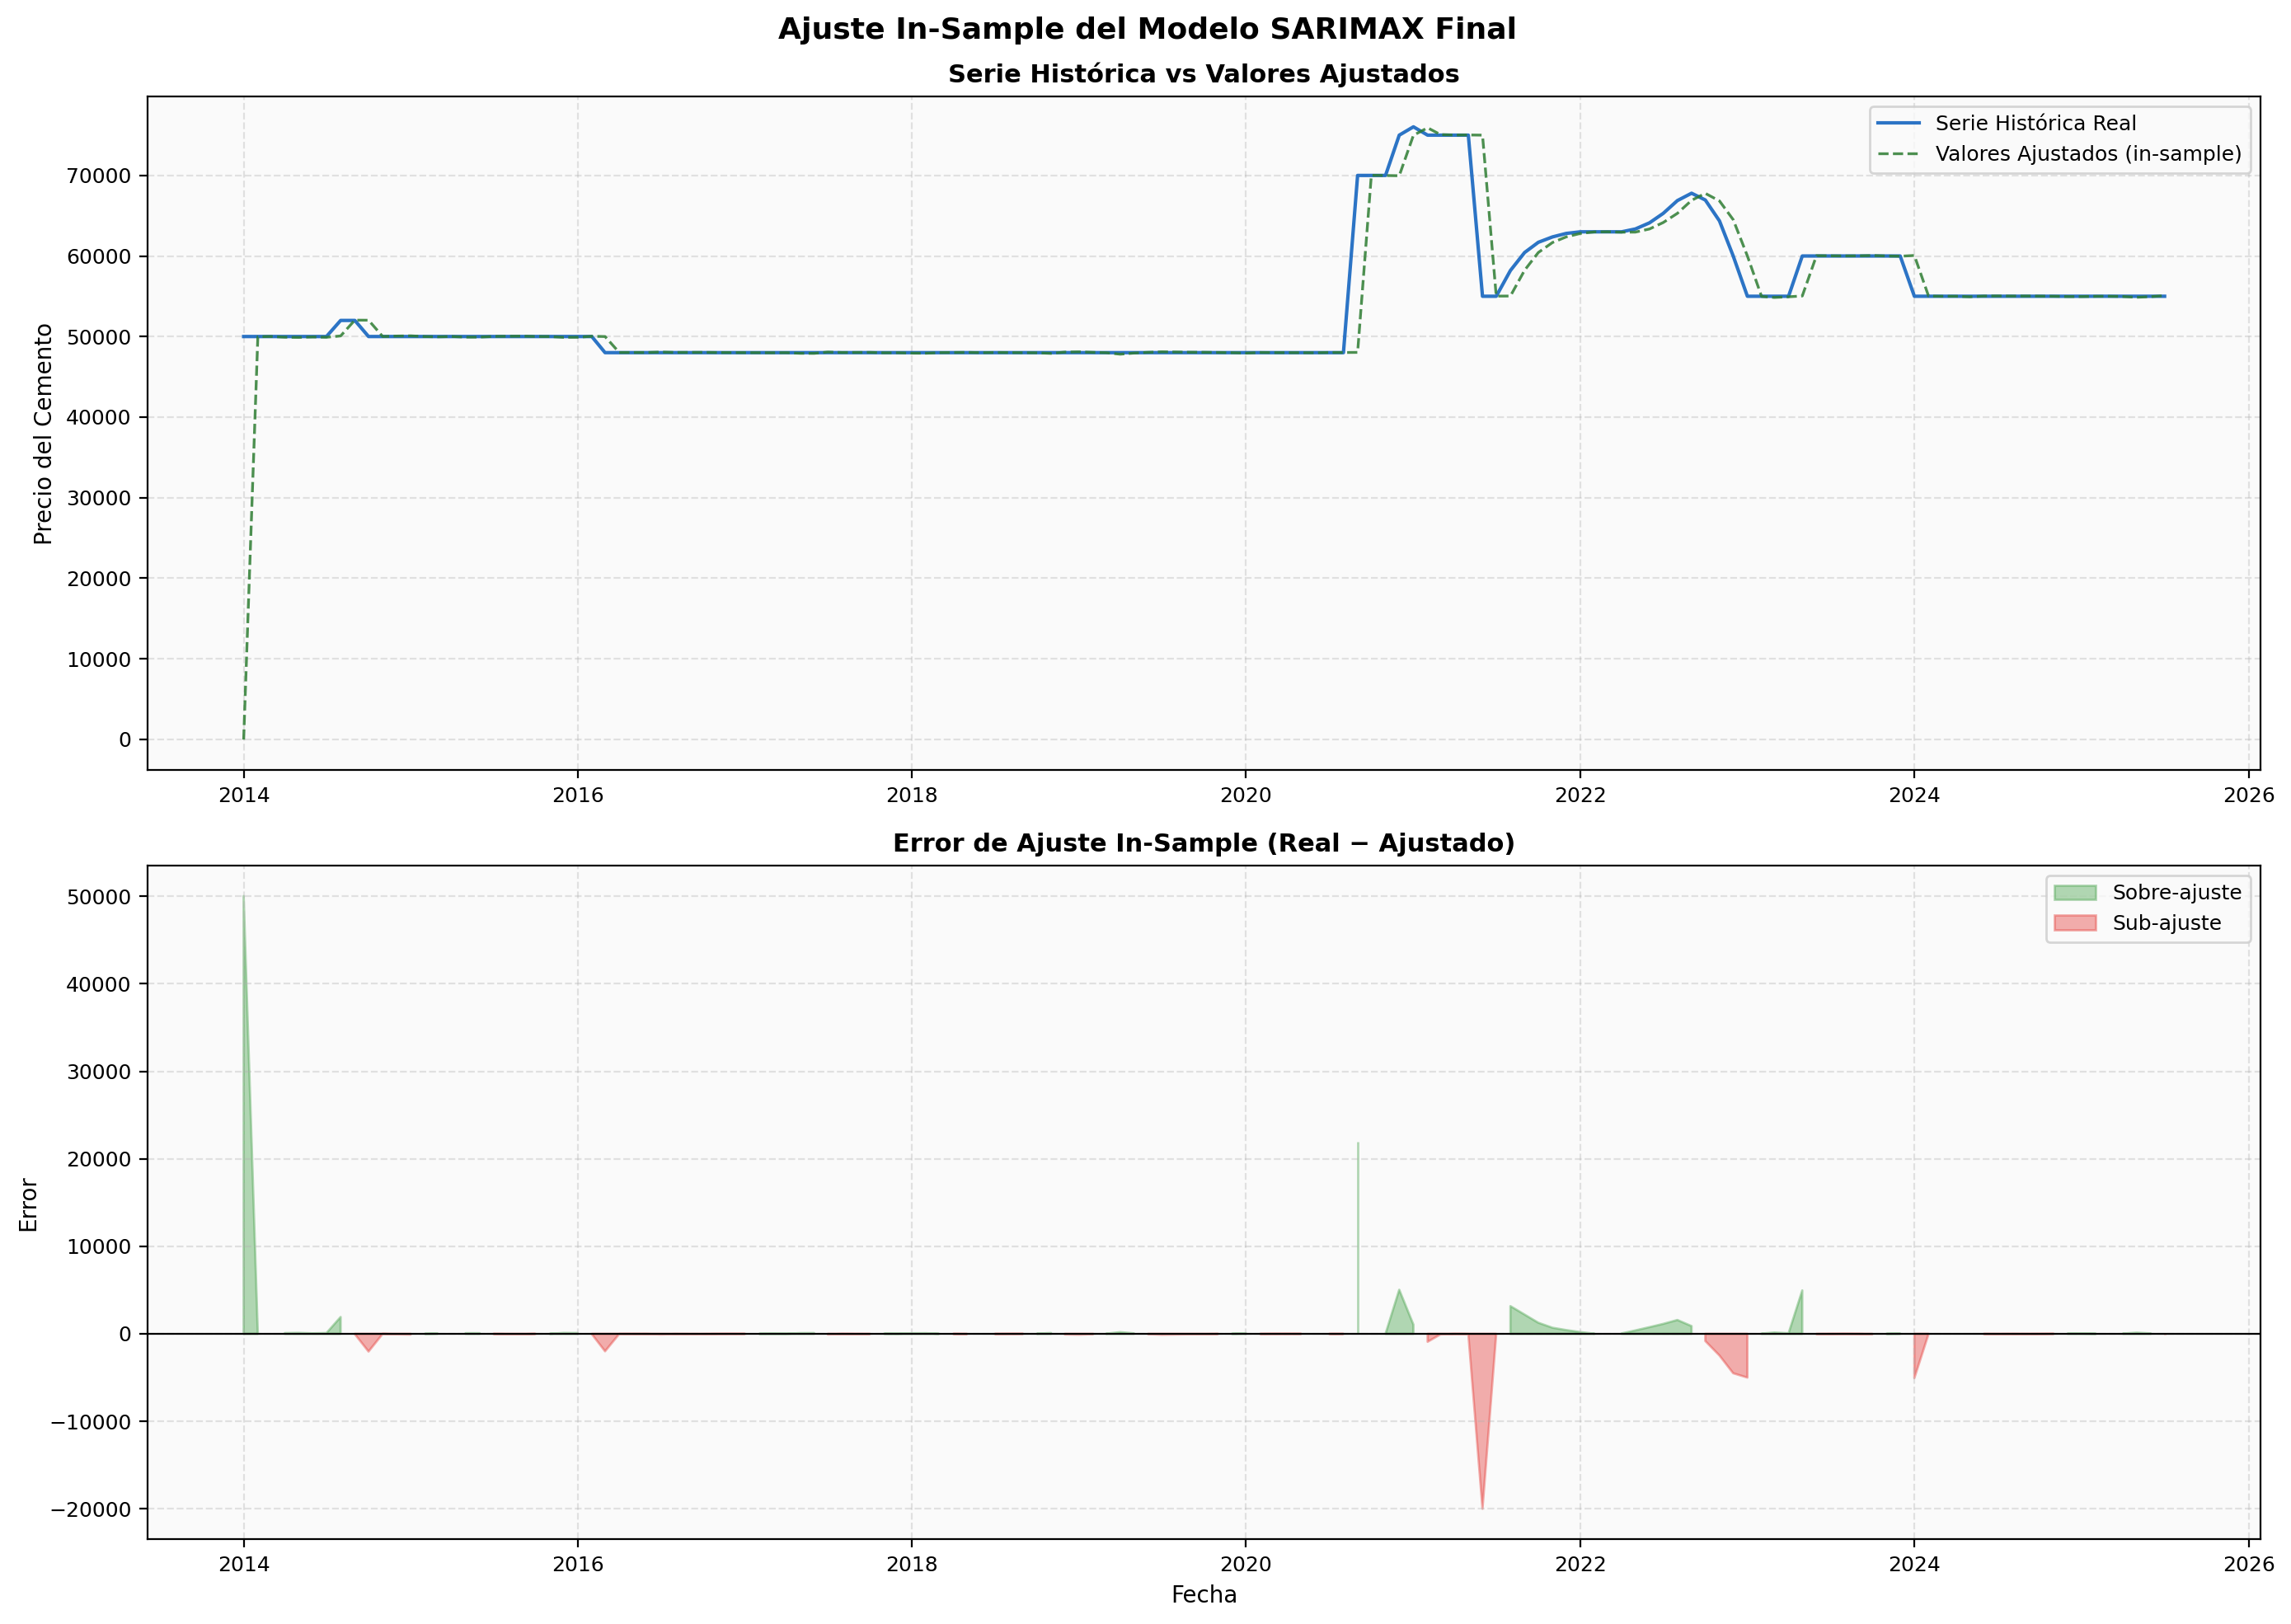
\includegraphics[width=\textwidth]{predicciones/prediccion_sarimax_cemento/graficos/11_ajuste_insample.png}
    \caption{Ajuste in-sample del modelo SARIMAX: valores reales versus valores ajustados sobre el período de entrenamiento.}
    \label{fig:sarimax_insample}
\end{figure}

\justify
La Figura \ref{fig:sarimax_insample} muestra el ajuste del modelo sobre los datos de entrenamiento. El modelo sigue con precisión la trayectoria histórica del precio del cemento, incluyendo la aceleración registrada en el período 2020--2022.

\begin{figure}[ht]
    \centering
    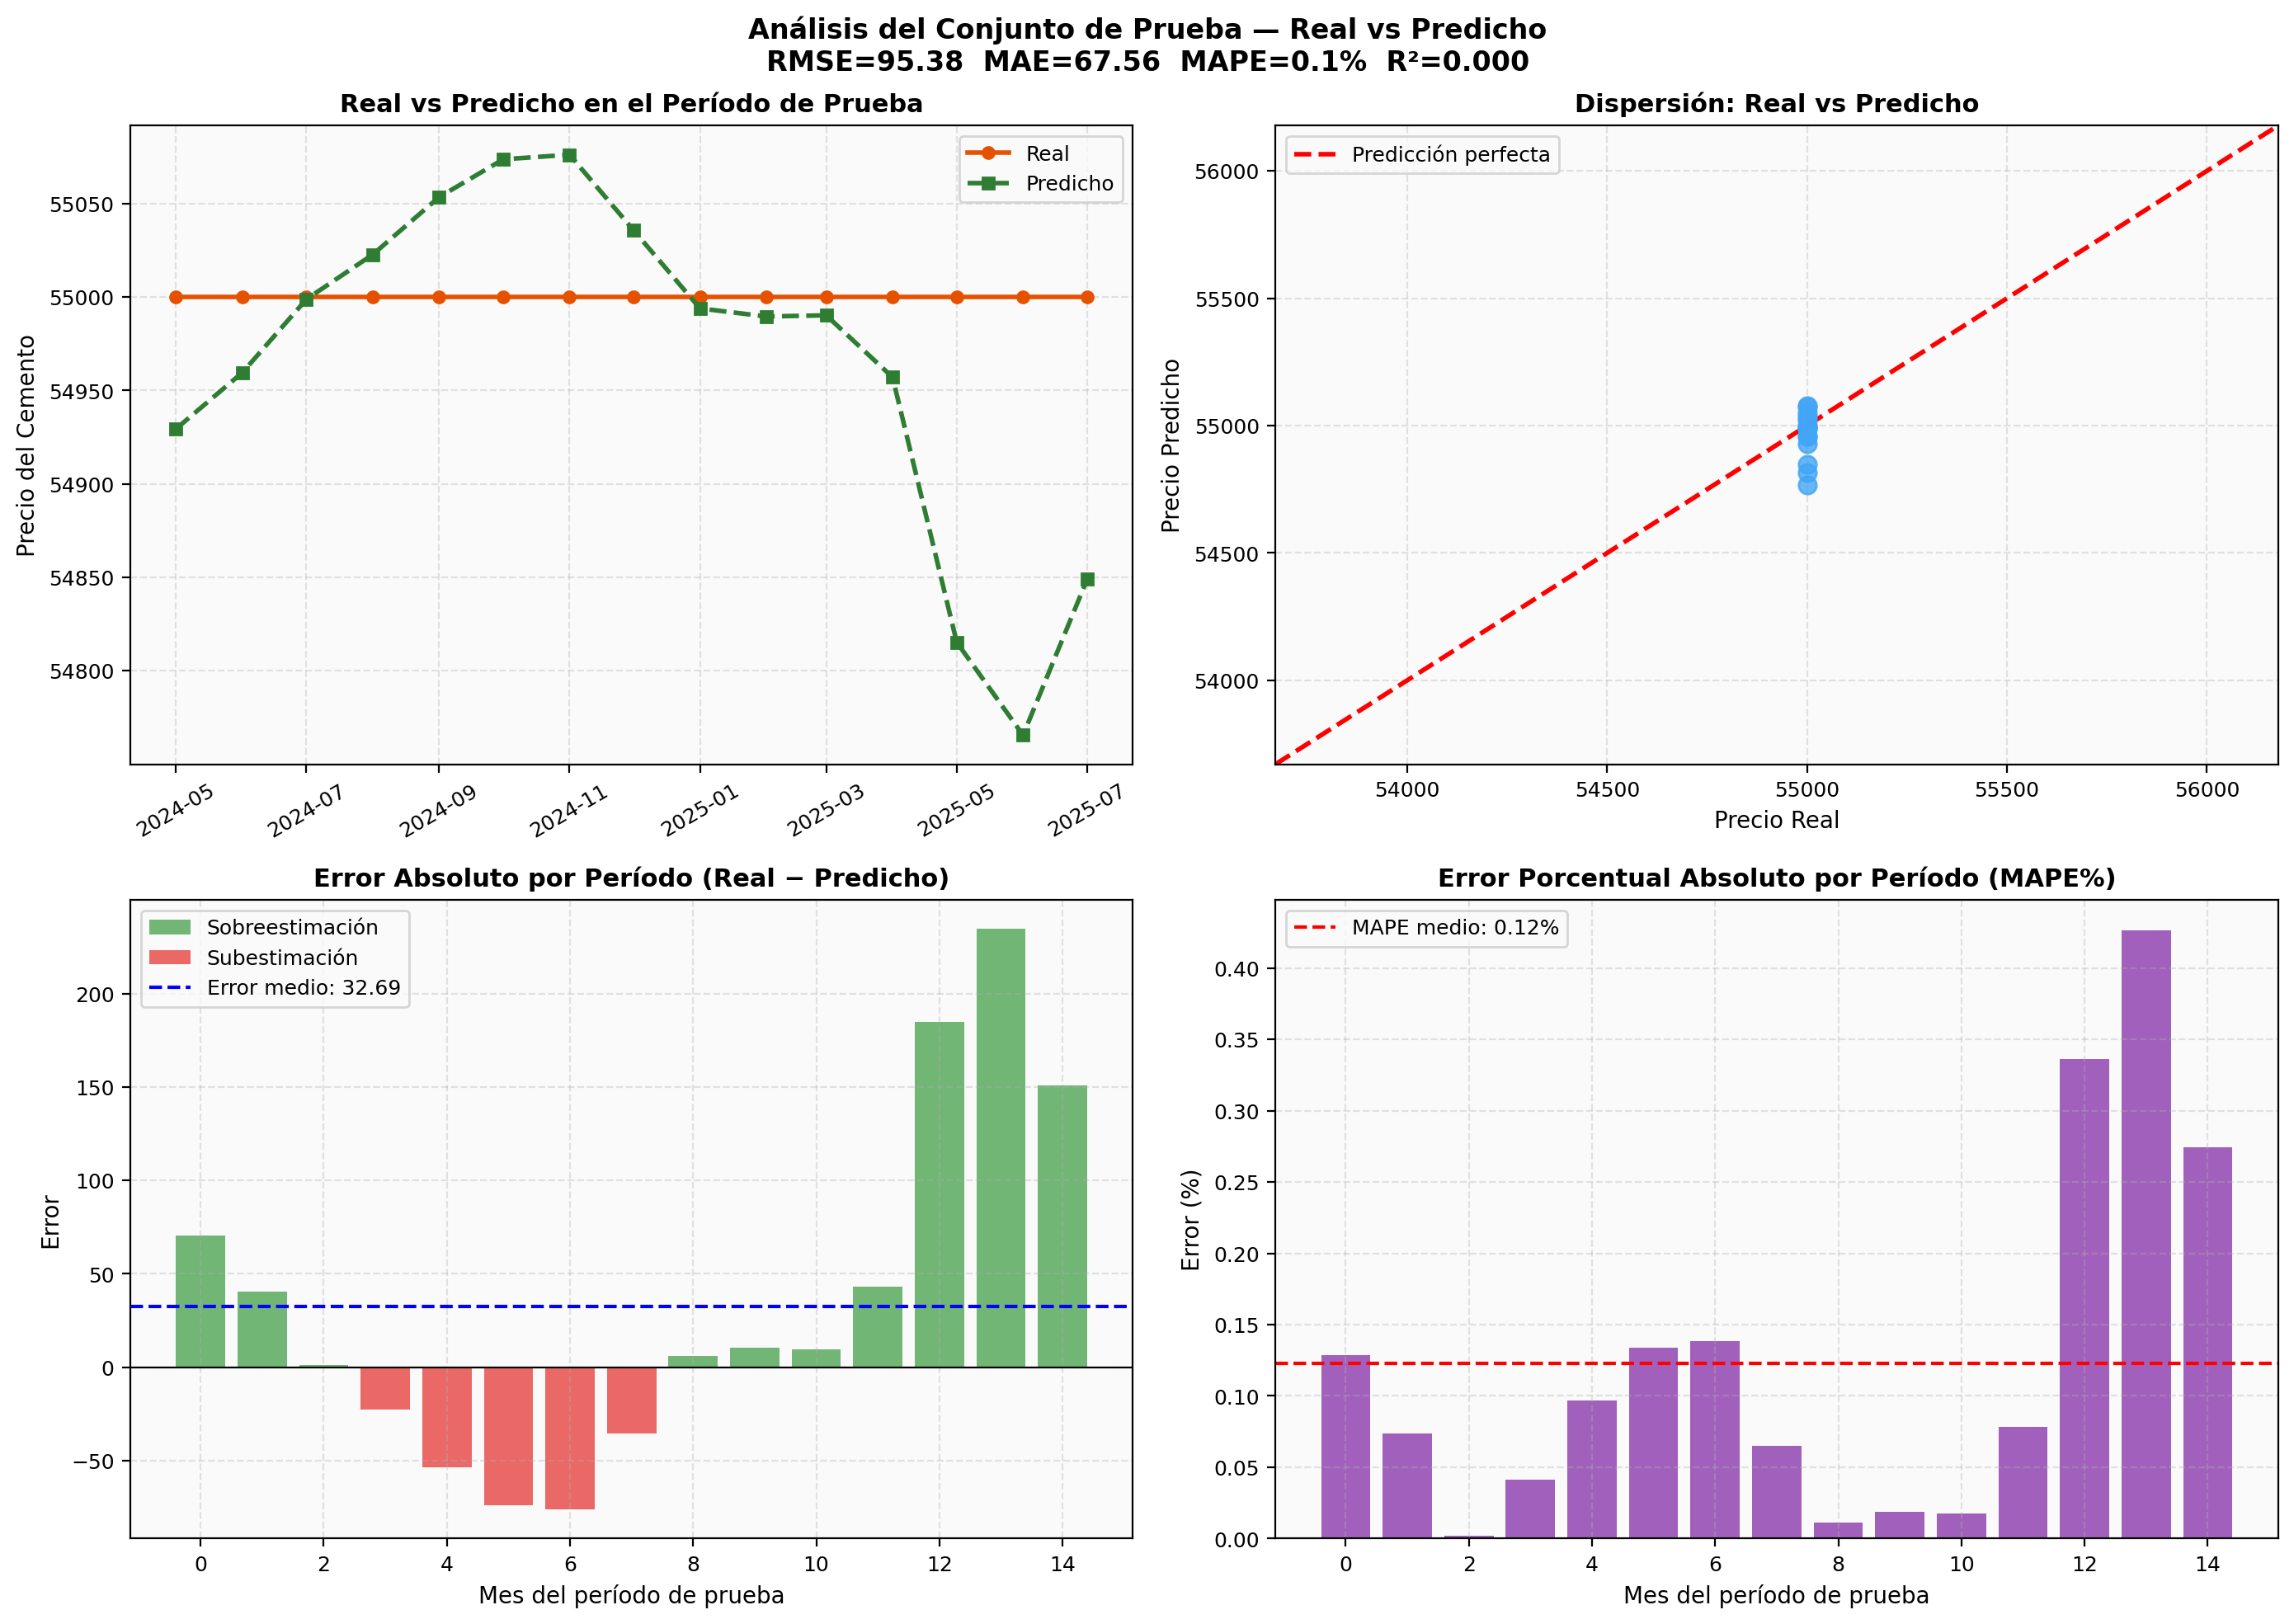
\includegraphics[width=\textwidth]{predicciones/prediccion_sarimax_cemento/graficos/08_comparacion_real_predicho.png}
    \caption{Comparación entre los valores reales y predichos del precio del cemento en el conjunto de prueba (15 meses).}
    \label{fig:sarimax_comparacion}
\end{figure}

\justify
La Figura \ref{fig:sarimax_comparacion} presenta la comparación entre los valores reales y los predichos por el modelo sobre el conjunto de prueba, que comprende los últimos 15 meses de la serie. Las métricas de evaluación obtenidas se resumen en la Tabla \ref{tab:sarimax_metricas_prueba}.

\begin{table}[ht]
    \centering
    \caption{Métricas de evaluación del modelo SARIMAX sobre el conjunto de prueba (15 meses).}
    \label{tab:sarimax_metricas_prueba}
    \begin{tabular}{lc}
        \toprule
        \textbf{Métrica} & \textbf{Valor} \\
        \midrule
        RMSE (Raíz del Error Cuadrático Medio) & 95{,}38~Gs. \\
        MAE  (Error Absoluto Medio)            & 67{,}56~Gs. \\
        MAPE (Error Porcentual Medio Absoluto) & 0{,}12\,\% \\
        SMAPE (Error Porcentual Simétrico)     & 0{,}12\,\% \\
        Error Absoluto Máximo                  & 234{,}47~Gs. \\
        $R^{2}$ (Coeficiente de Determinación) & 0{,}0000 \\
        \bottomrule
    \end{tabular}
\end{table}

\justify
El MAPE de 0{,}12\,\% sobre el conjunto de prueba merece una lectura cuidadosa. Tomado en aislamiento, parece un resultado excelente: las predicciones se alejan poco más de una décima de punto porcentual del valor real. El RMSE de 95{,}38~Gs. y el MAE de 67{,}56~Gs. también son bajos respecto al rango histórico de la serie (Gs.~48.000--76.036). Sin embargo, el $R^{2}=0$ en el mismo período llama la atención: ¿cómo puede el modelo tener un error relativo tan bajo y al mismo tiempo un $R^{2}$ nulo?

\justify
La explicación es que, en el período de prueba, el precio del cemento se mantuvo prácticamente estable — varianza muy baja — de modo que cualquier predicción constante cercana al nivel reciente resultará en errores absolutos pequeños, pero sin diferenciarse del simple promedio histórico en términos de varianza explicada. En otras palabras, el contexto del mercado durante ese período limitó lo que cualquier modelo, no solo el SARIMAX, podía demostrar. El comportamiento es además coherente con el orden $(0,1,0)$ seleccionado: sin términos AR ni MA, el modelo proyecta básicamente el último valor observado, que es la estrategia óptima cuando la serie diferenciada se comporta como ruido blanco. La validación cruzada, que sí abarca períodos con mayor variabilidad, ofrece una imagen más completa del desempeño real.

\subsubsection{Modelo SARIMAX: Validación Cruzada}

\begin{figure}[ht]
    \centering
    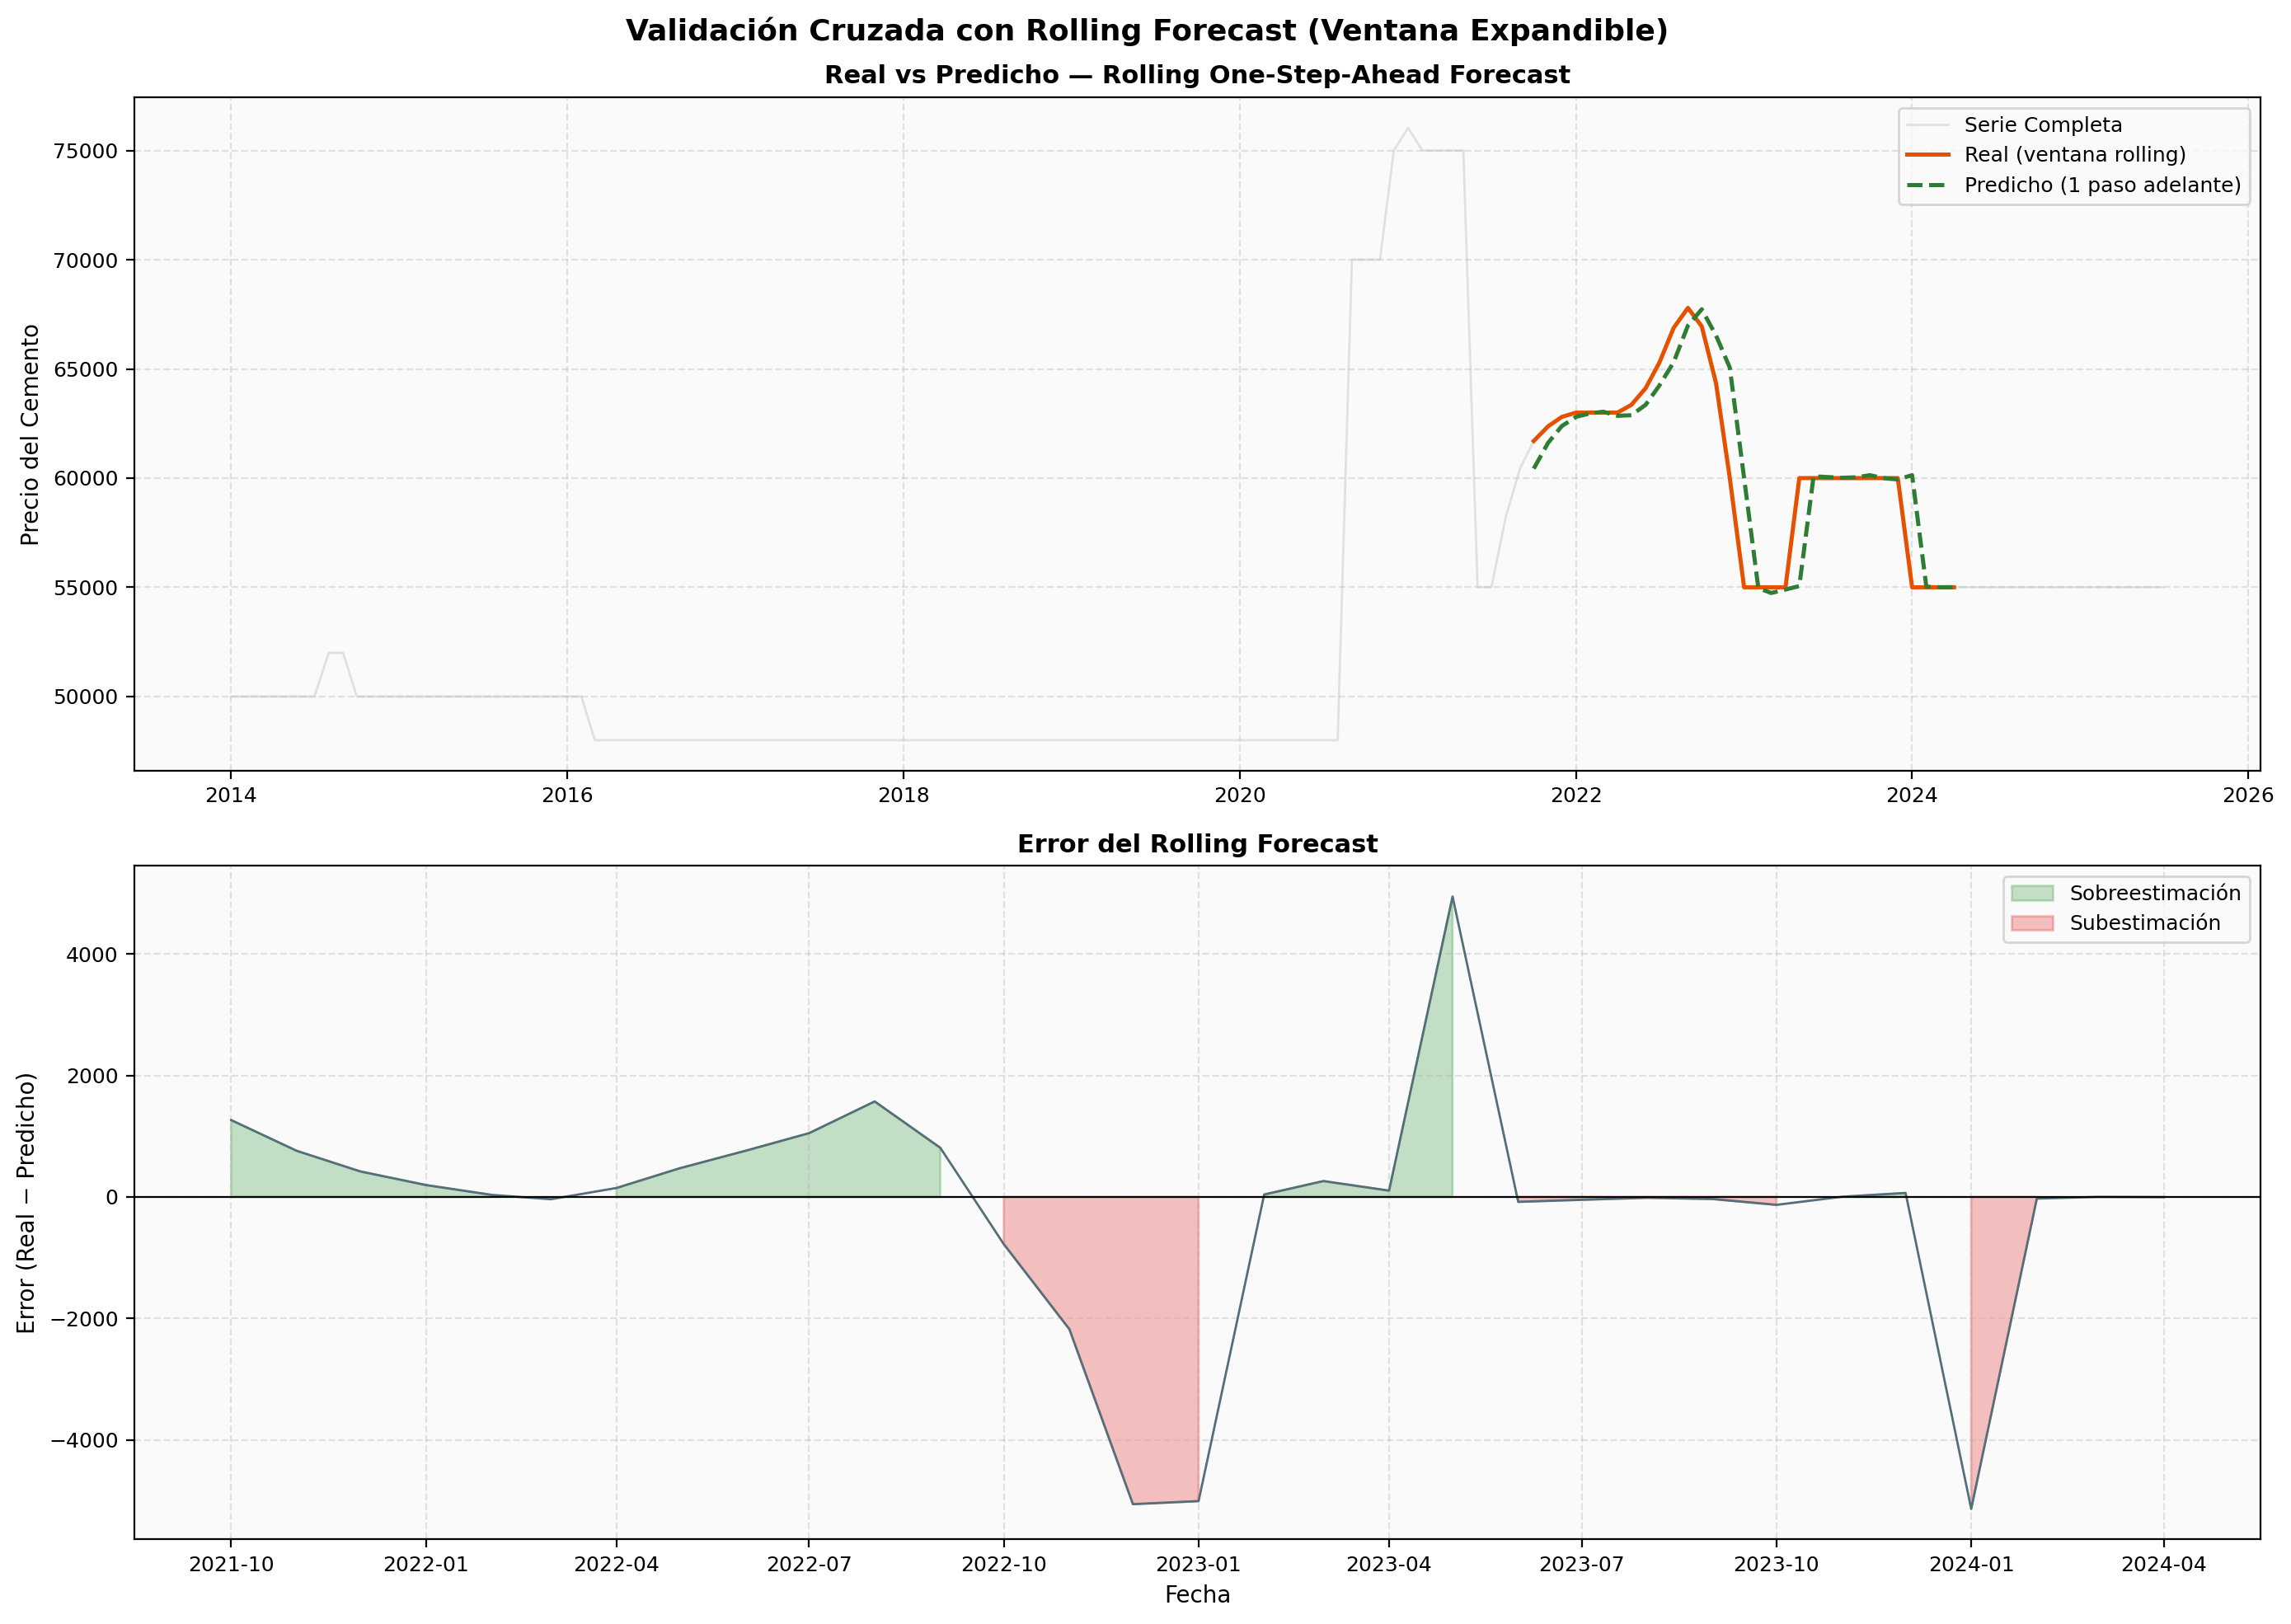
\includegraphics[width=\textwidth]{predicciones/prediccion_sarimax_cemento/graficos/10_rolling_forecast_cv.png}
    \caption{Validación cruzada por ventana deslizante (\textit{rolling forecast}): predicciones puntuales versus valores reales en cada paso de avance.}
    \label{fig:sarimax_rolling}
\end{figure}

\justify
Con el fin de obtener una estimación más robusta de la capacidad predictiva del modelo, se aplicó una validación cruzada por ventana deslizante (\textit{rolling forecast}), en la que el modelo se re-estima en cada paso incorporando las observaciones disponibles hasta ese momento y genera una predicción un paso adelante. La Figura \ref{fig:sarimax_rolling} ilustra el resultado de este procedimiento. Las métricas obtenidas se presentan en la Tabla \ref{tab:sarimax_metricas_cv}.

\begin{table}[ht]
    \centering
    \caption{Métricas de validación cruzada por ventana deslizante del modelo SARIMAX.}
    \label{tab:sarimax_metricas_cv}
    \begin{tabular}{lc}
        \toprule
        \textbf{Métrica} & \textbf{Valor} \\
        \midrule
        RMSE & 1.920{,}78~Gs. \\
        MAE  & 1.013{,}86~Gs. \\
        MAPE & 1{,}70\,\% \\
        $R^{2}$ & 0{,}7586 \\
        \bottomrule
    \end{tabular}
\end{table}

\justify
Aquí el panorama cambia. Con un $R^{2}=0{,}7586$, el modelo explica el 75{,}86\,\% de la varianza del precio a lo largo de todo el período histórico disponible, incluyendo los años de alta volatilidad. El MAPE de 1{,}70\,\% —muy por debajo del umbral del 5\,\% que suele citarse como referencia para series de precios de materiales— confirma que el SARIMAX tiene utilidad práctica real para la gestión de presupuestos de obra, al menos en escenarios de proyección a un paso adelante.

\subsubsection{Modelo SARIMAX: Análisis de Residuos}

\begin{figure}[ht]
    \centering
    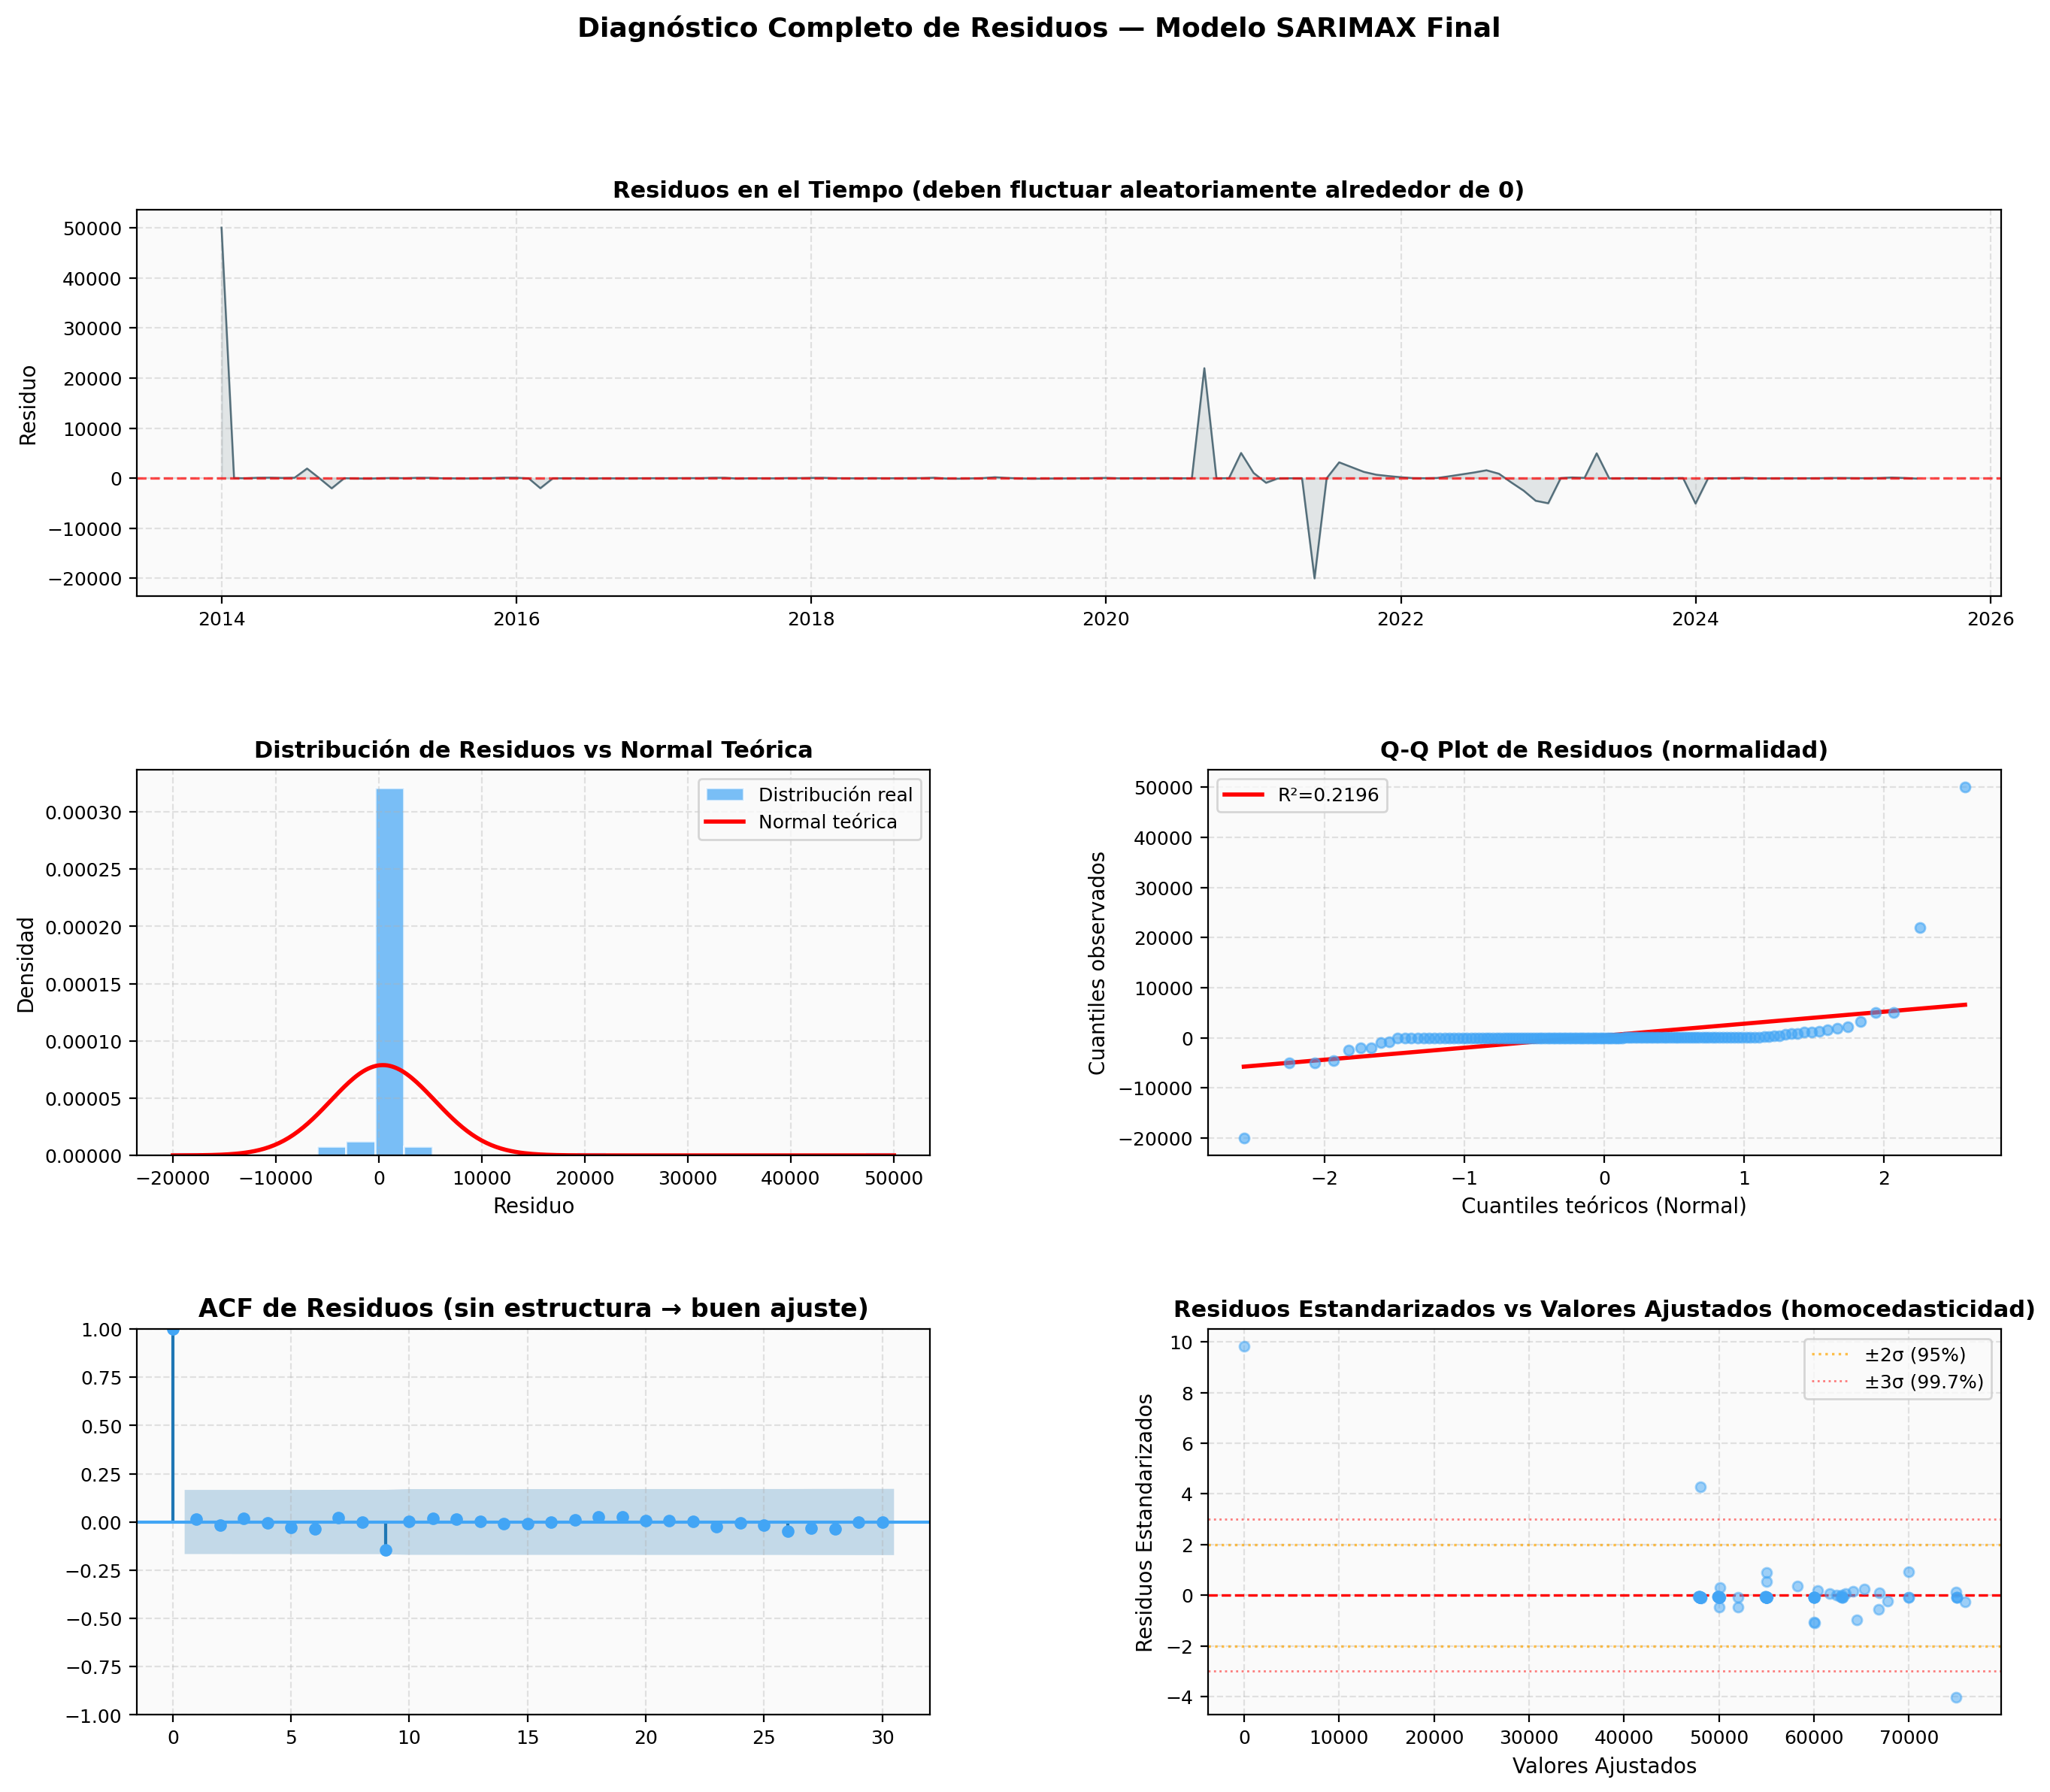
\includegraphics[width=\textwidth]{predicciones/prediccion_sarimax_cemento/graficos/07_diagnostico_residuos.png}
    \caption{Diagnóstico de residuos del modelo SARIMAX: gráfico de residuos, histograma, gráfico Q-Q y función de autocorrelación.}
    \label{fig:sarimax_residuos}
\end{figure}

\justify
La Figura \ref{fig:sarimax_residuos} presenta el diagnóstico completo de los residuos del modelo SARIMAX. El test de Ljung-Box no rechaza la hipótesis nula de ausencia de autocorrelación serial en los residuos para los rezagos 10 ($Q=3{,}77$, $p=0{,}957$) y 20 ($Q=4{,}13$, $p=0{,}9999$), confirmando que los residuos se comportan como ruido blanco y que el modelo ha capturado adecuadamente la estructura dinámica de la serie. Por su parte, el test de Shapiro-Wilk rechaza la normalidad de los residuos ($W=0{,}2404$, $p<0{,}001$), resultado que se explica por la presencia de observaciones extremas durante el período pandémico, las cuales introducen una curtosis elevada (49{,}47) y una asimetría positiva moderada (0{,}83). Esta no normalidad no invalida las estimaciones puntuales del modelo, aunque sí impone cautela en la interpretación de los intervalos de confianza calculados bajo el supuesto gaussiano.

\subsubsection{Modelo SARIMAX: Pronóstico a 24 Meses}

\begin{figure}[ht]
    \centering
    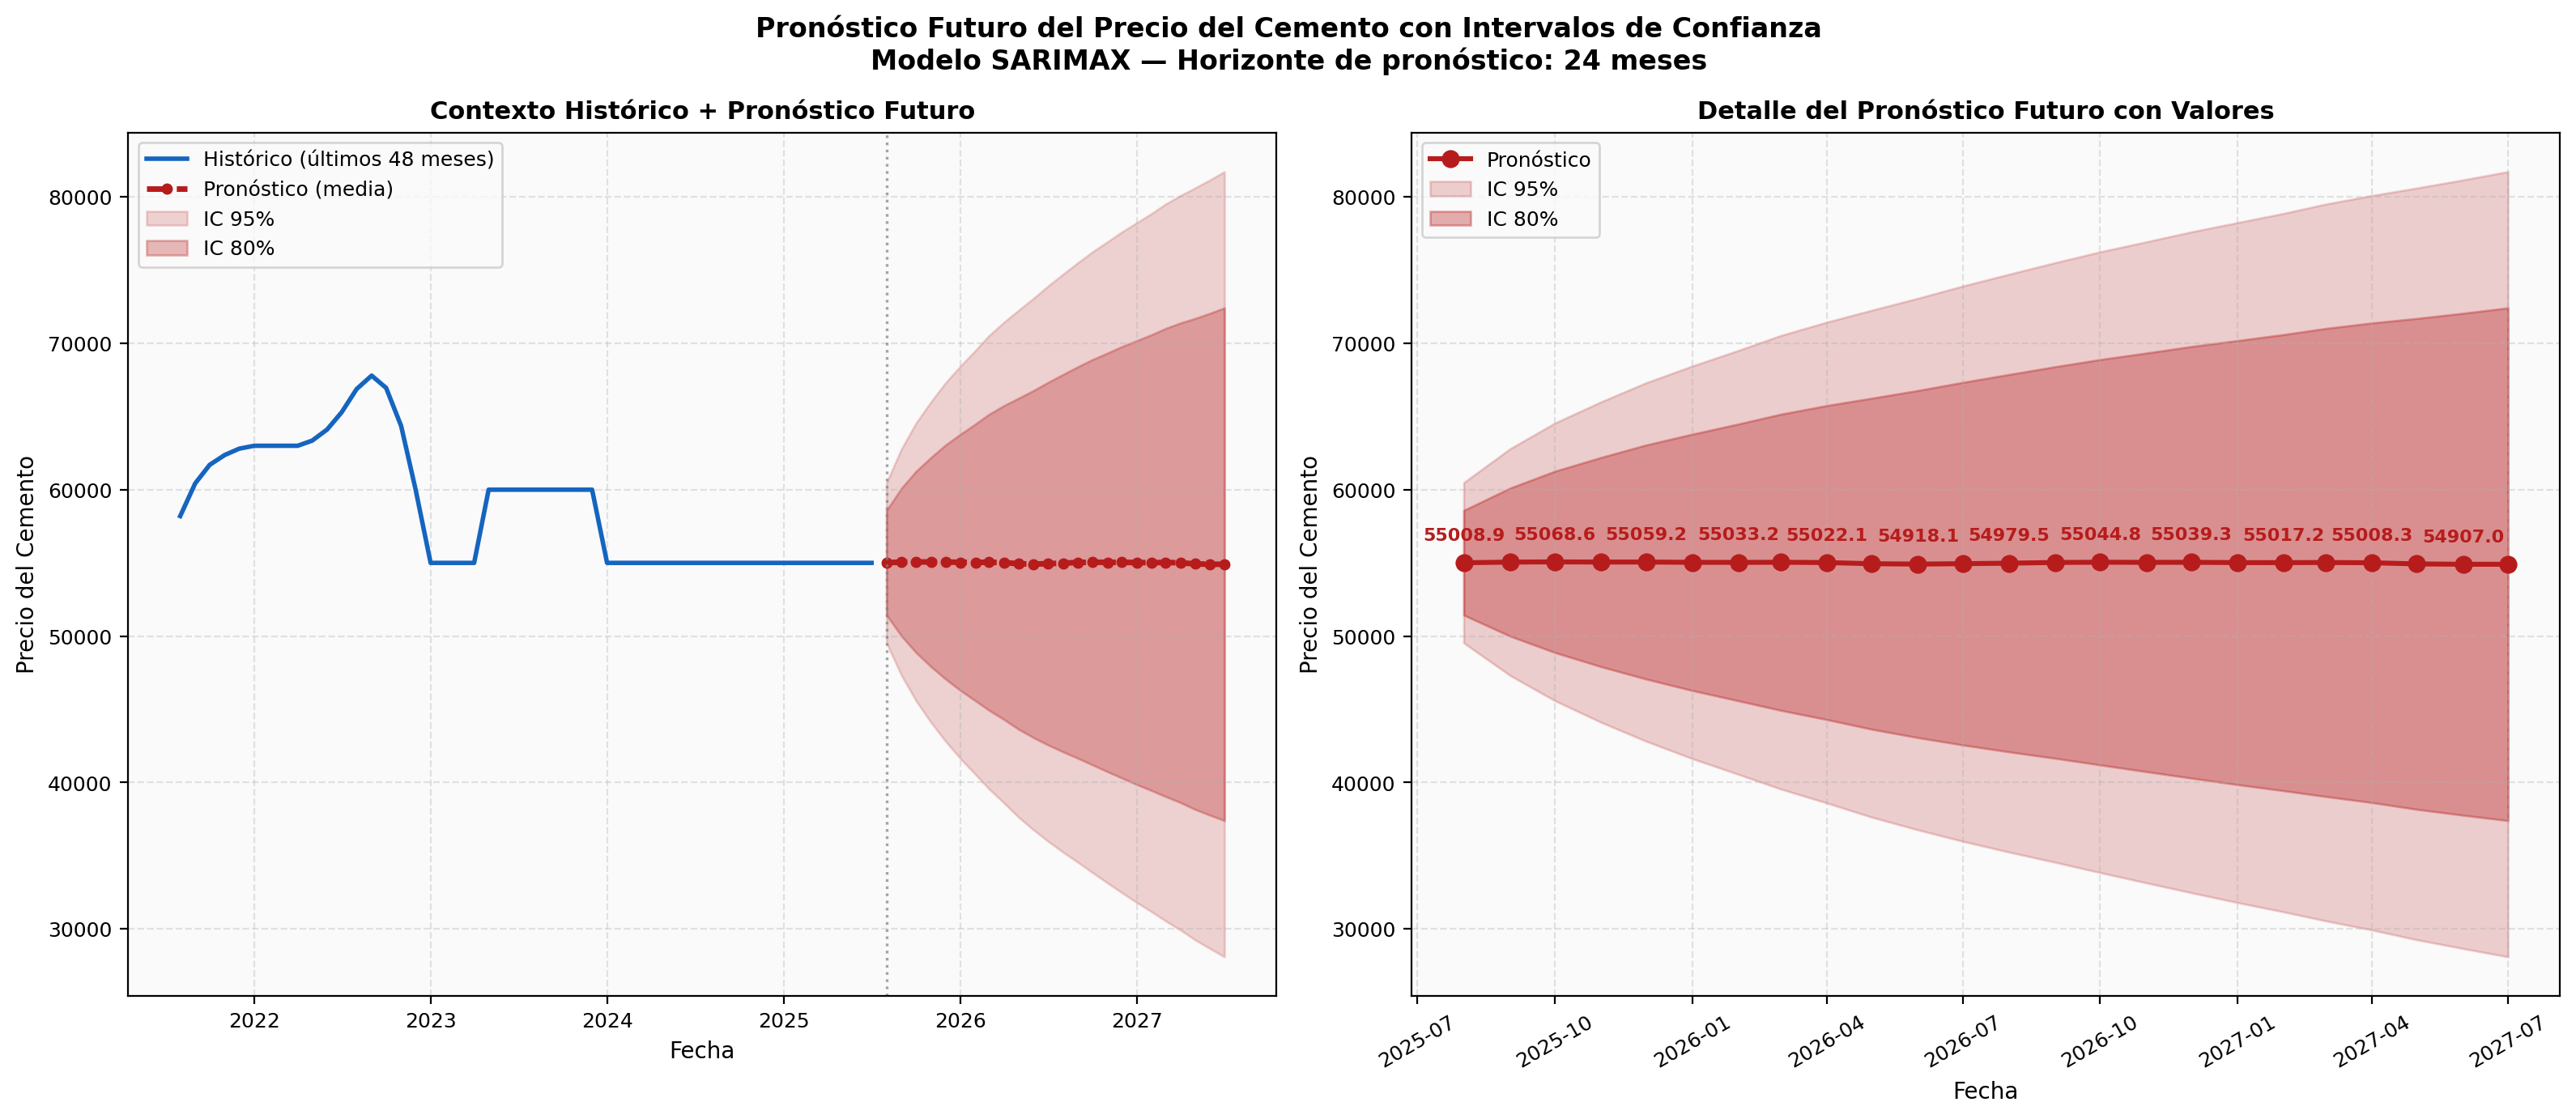
\includegraphics[width=\textwidth]{predicciones/prediccion_sarimax_cemento/graficos/09_pronostico_intervalo_confianza.png}
    \caption{Pronóstico del precio del cemento a 24 meses (agosto 2025 -- julio 2027) con intervalos de confianza al 95\%.}
    \label{fig:sarimax_pronostico_ic}
\end{figure}

\begin{figure}[ht]
    \centering
    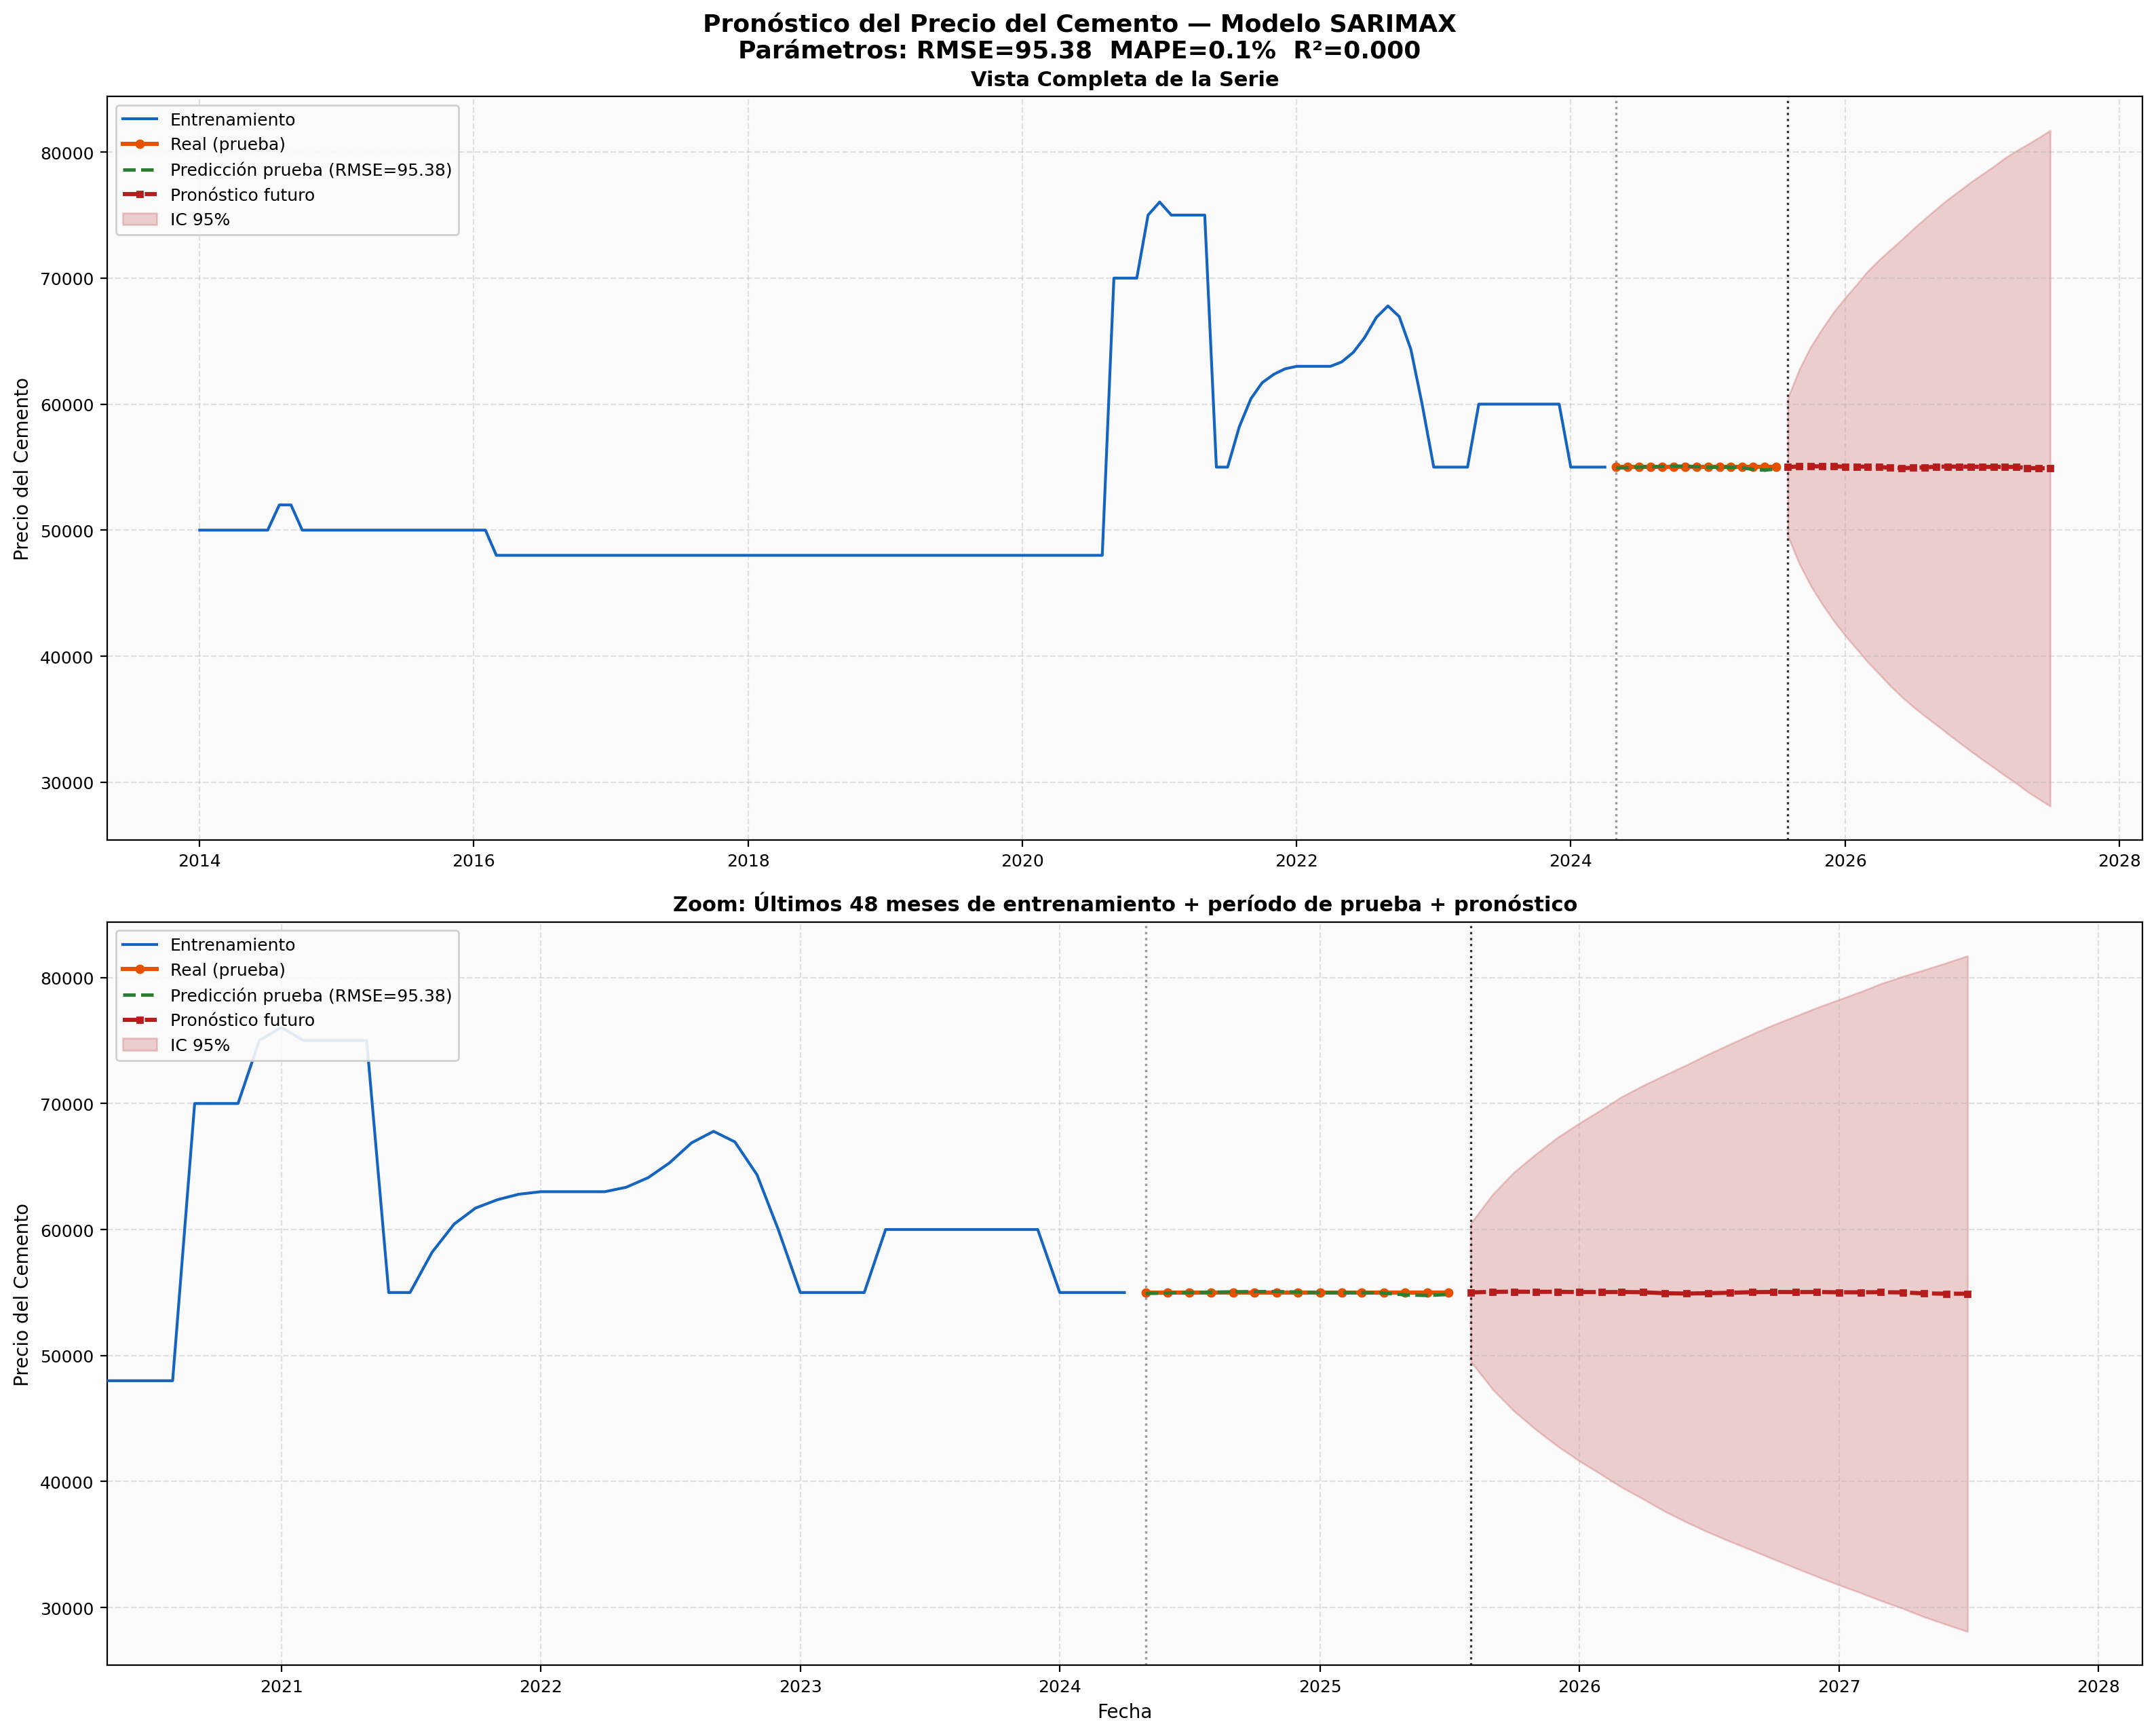
\includegraphics[width=\textwidth]{predicciones/prediccion_sarimax_cemento/graficos/06_pronostico_completo.png}
    \caption{Pronóstico completo del precio del cemento: serie histórica observada y proyección SARIMAX a 24 meses.}
    \label{fig:sarimax_pronostico_completo}
\end{figure}

\justify
Una vez validado el modelo, se generó el pronóstico del precio mensual del cemento para el horizonte de 24 meses comprendido entre agosto de 2025 y julio de 2027, utilizando como variable exógena los niveles del río Paraguay proyectados por el modelo LSTM. Las Figuras \ref{fig:sarimax_pronostico_ic} y \ref{fig:sarimax_pronostico_completo} presentan el pronóstico puntual y el intervalo de confianza al 95\,\%, así como la vista conjunta con la serie histórica completa.

\justify
El pronóstico puntual converge rápidamente hacia un valor estable de aproximadamente Gs.~55.010, consistente con la naturaleza del modelo SARIMAX$(0,1,0)$, cuyas predicciones corresponden a la última observación más la contribución de las variables exógenas proyectadas. El intervalo de confianza al 95\,\% se amplía progresivamente con el horizonte de predicción: para agosto de 2025 el rango es de Gs.~[49.535 -- 60.483], mientras que para julio de 2027 se extiende a Gs.~[28.089 -- 81.724]. Este ensanchamiento, inherente a los modelos integrados en horizontes largos, refleja la incertidumbre acumulada de la proyección y proporciona los límites inferior y superior necesarios para la planificación conservadora y optimista de presupuestos de obra.

\justify
La Tabla \ref{tab:sarimax_pronostico} sintetiza los valores pronosticados para los primeros doce meses del horizonte de predicción.

\begin{table}[ht]
    \centering
    \caption{Pronóstico mensual del precio del cemento (Gs.) para el período agosto 2025 -- julio 2026, con intervalo de confianza al 95\,\%.}
    \label{tab:sarimax_pronostico}
    \begin{tabular}{lccc}
        \toprule
        \textbf{Mes} & \textbf{Pronóstico (Gs.)} & \textbf{IC Inferior} & \textbf{IC Superior} \\
        \midrule
        Agosto 2025      & 55.009 & 49.535 & 60.483 \\
        Septiembre 2025  & 55.053 & 47.311 & 62.794 \\
        Octubre 2025     & 55.069 & 45.587 & 64.550 \\
        Noviembre 2025   & 55.055 & 44.107 & 66.003 \\
        Diciembre 2025   & 55.059 & 42.819 & 67.299 \\
        Enero 2026       & 55.037 & 41.628 & 68.445 \\
        Febrero 2026     & 55.033 & 40.550 & 69.516 \\
        Marzo 2026       & 55.041 & 39.558 & 70.524 \\
        Abril 2026       & 55.022 & 38.600 & 71.444 \\
        Mayo 2026        & 54.942 & 37.632 & 72.253 \\
        Junio 2026       & 54.918 & 36.763 & 73.073 \\
        Julio 2026       & 54.946 & 35.983 & 73.908 \\
        \bottomrule
    \end{tabular}
\end{table}

\subsubsection{Modelo SARIMAX: Escenarios con y sin Efecto Pandémico}

\justify
Con el fin de evaluar la sensibilidad del pronóstico SARIMAX ante el \textit{shock} pandémico, se generaron dos proyecciones paralelas: una con la variable \texttt{Cuarentena} fijada en cero (escenario sin pandemia) y otra con esta variable activa durante todo el horizonte de pronóstico (escenario con efecto pandémico). Las Figuras \ref{fig:sarimax_cemento_sin_covid} y \ref{fig:sarimax_cemento_con_covid} presentan los pronósticos resultantes para cada escenario.

\begin{figure}[ht]
    \centering
    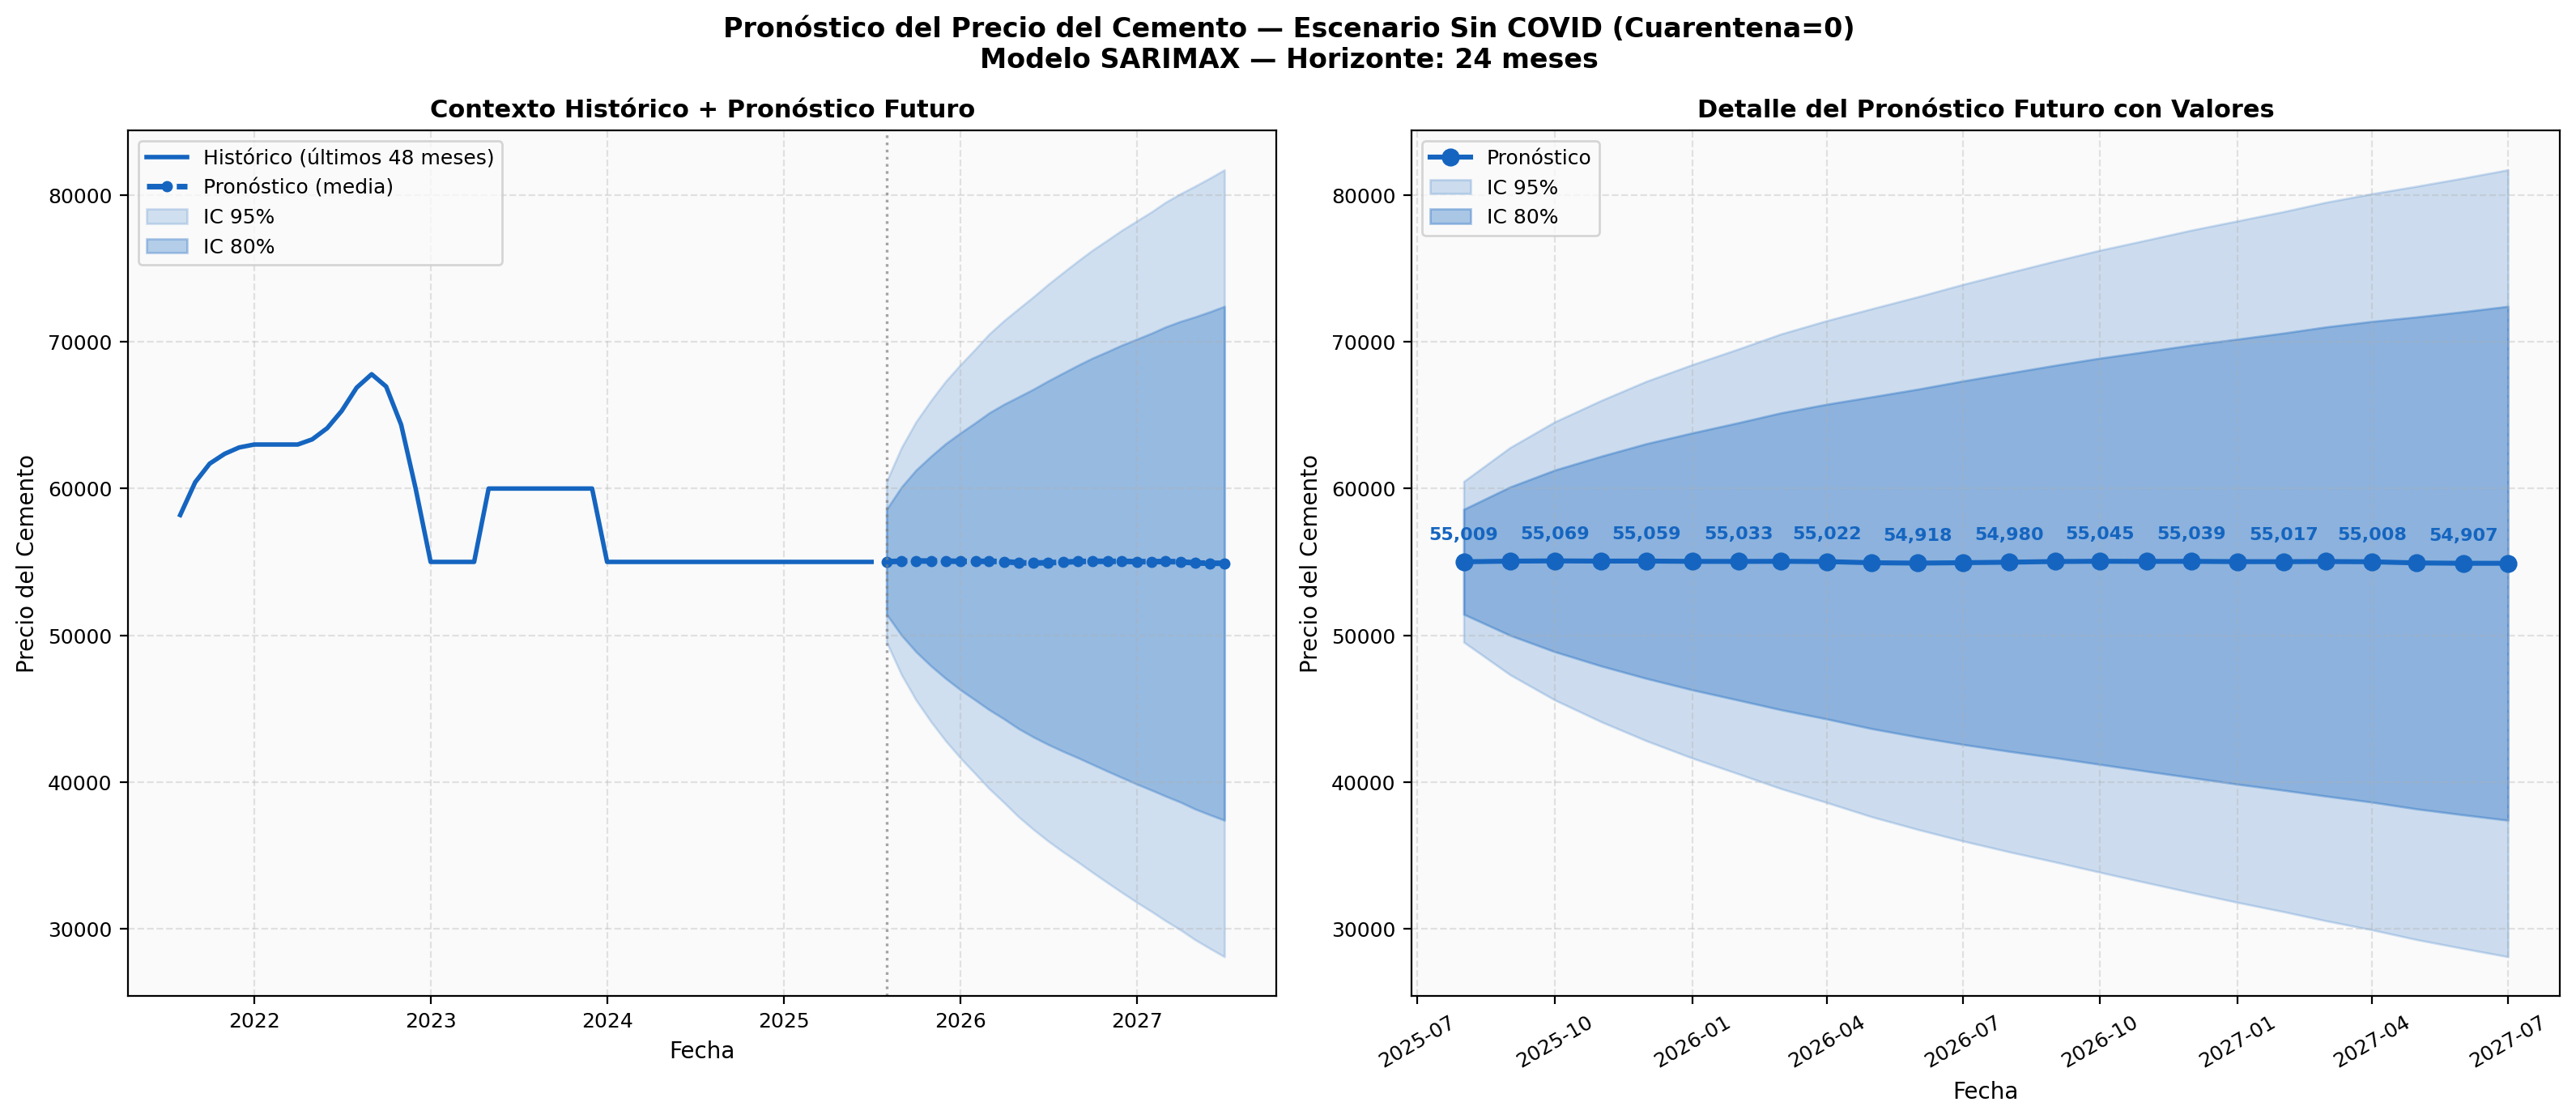
\includegraphics[width=\textwidth]{predicciones/prediccion_sarimax_cemento/graficos/12a_pronostico_sin_covid.png}
    \caption{Pronóstico SARIMAX del precio del cemento a 24 meses -- escenario sin efecto pandémico.}
    \label{fig:sarimax_cemento_sin_covid}
\end{figure}

\begin{figure}[ht]
    \centering
    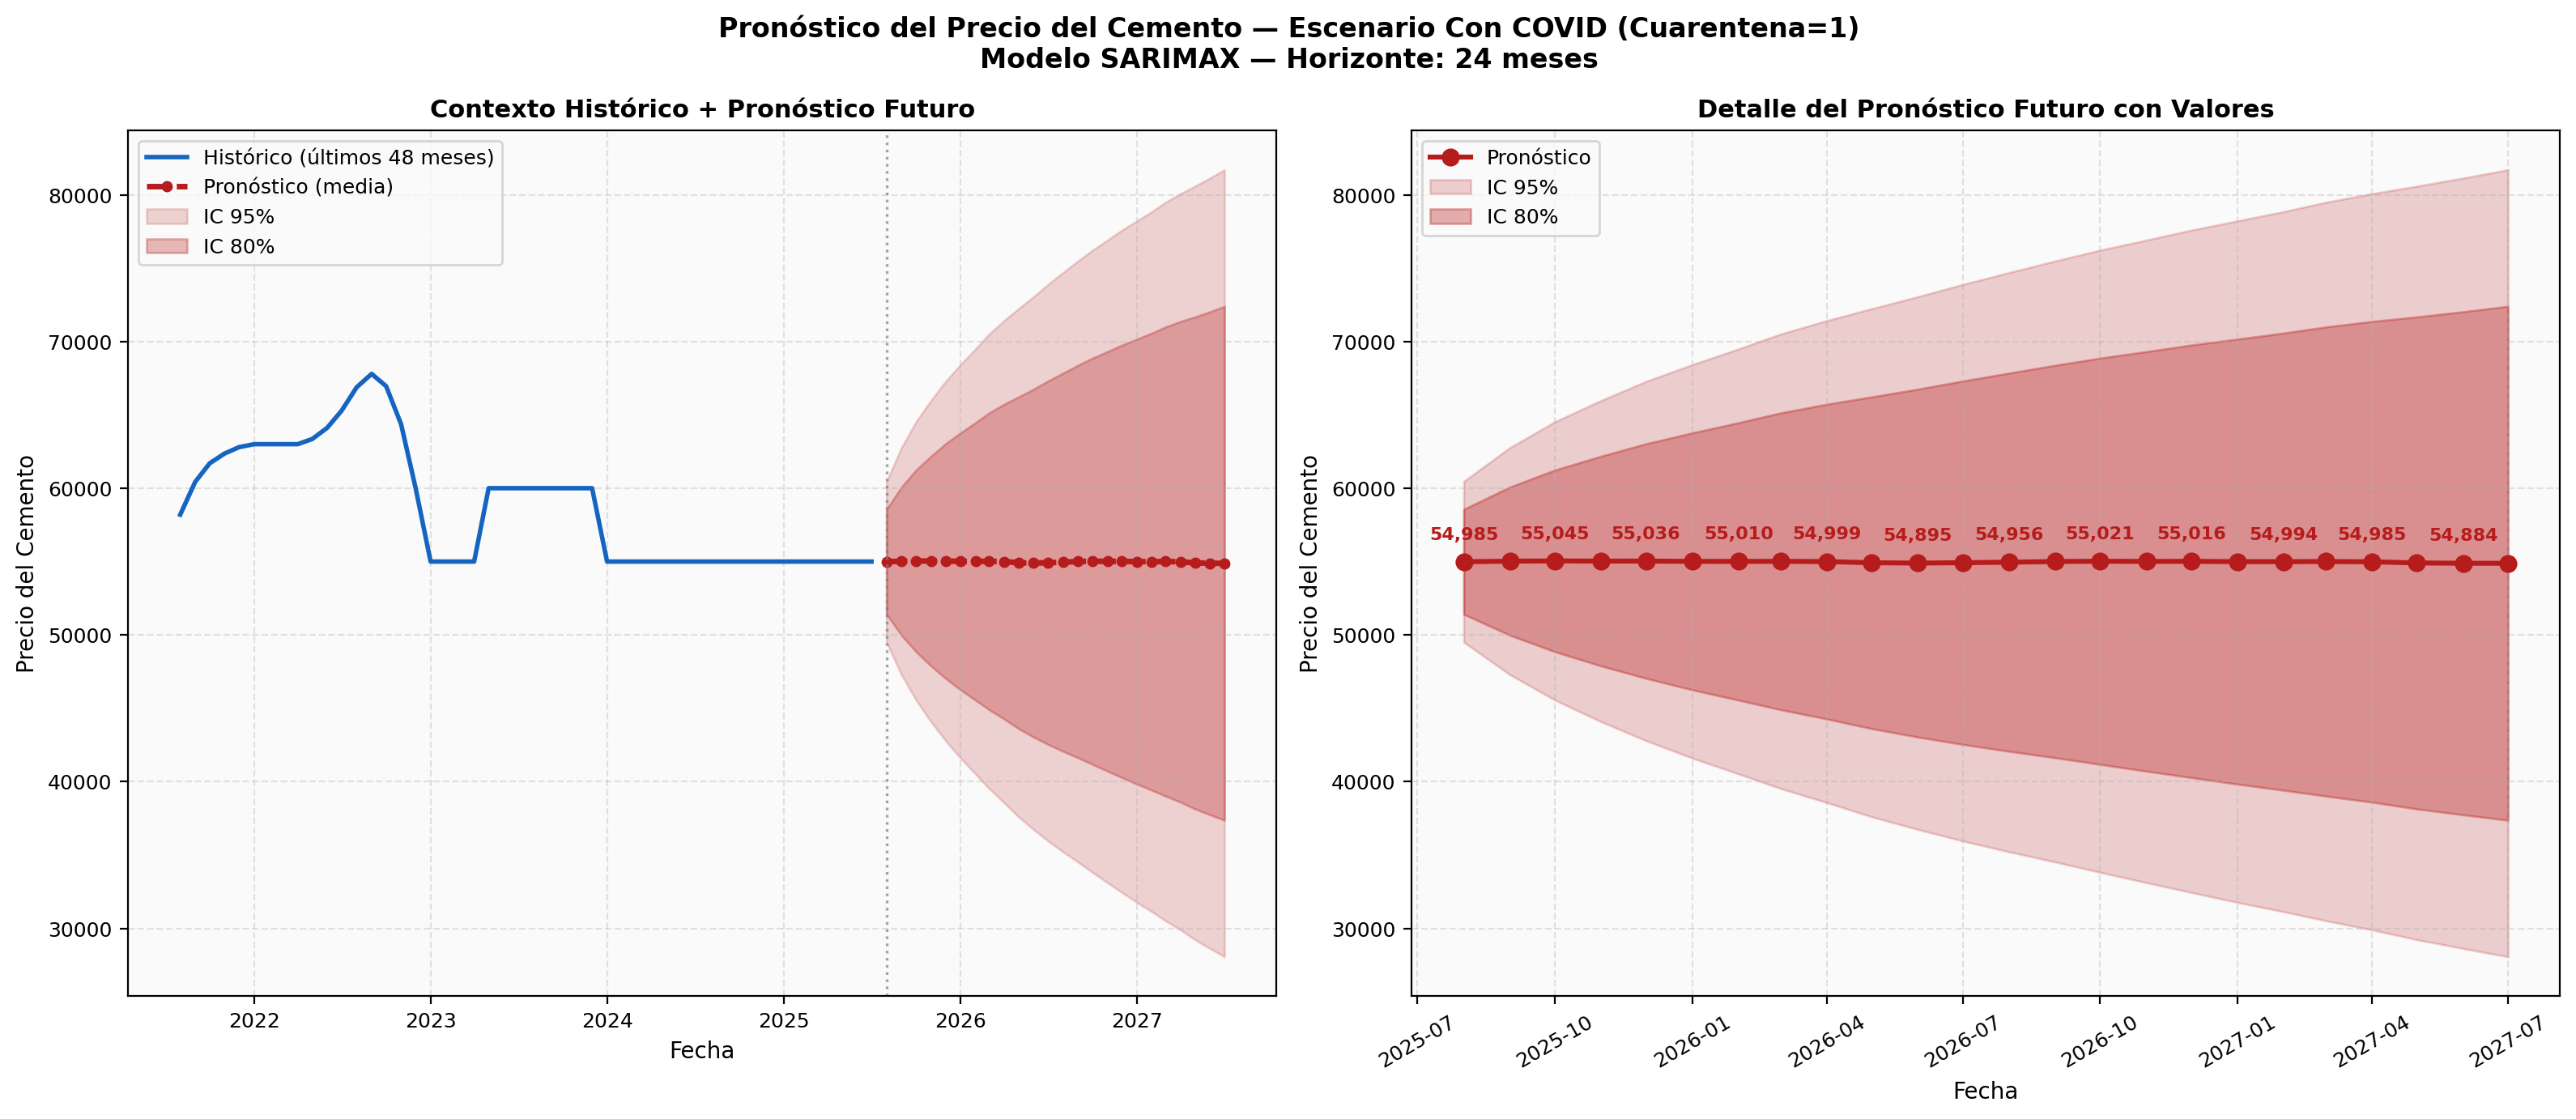
\includegraphics[width=\textwidth]{predicciones/prediccion_sarimax_cemento/graficos/12b_pronostico_con_covid.png}
    \caption{Pronóstico SARIMAX del precio del cemento a 24 meses -- escenario con efecto pandémico.}
    \label{fig:sarimax_cemento_con_covid}
\end{figure}

\justify
El resultado es revelador: la diferencia entre ambos escenarios es de apenas Gs.~$-23{,}48$ por mes, un valor prácticamente despreciable frente al nivel de precios de la serie (Gs.~55.000). Esta diferencia mínima es consistente con el hecho de que el coeficiente estimado para la variable \texttt{Cuarentena} en el modelo SARIMAX resultó estadísticamente no significativo ($p=1{,}000$), como se documentó en la Tabla \ref{tab:sarimax_params}. En otras palabras, el modelo lineal integrado no logra capturar el efecto estructural de la pandemia sobre los precios, dado que la mayor parte de ese impacto queda absorbida por la diferenciación de la serie ($d=1$). Esta limitación del SARIMAX para representar \textit{shocks} exógenos persistentes constituye una de las motivaciones principales para explorar los modelos de aprendizaje profundo, los cuales sí pueden capturar interacciones no lineales entre la variable pandémica y la dinámica de precios.

% ============================================================
\subsection{Predicción del Precio del Ladrillo}
\vspace{0.3cm}
\justify
Además del cemento, se modeló el precio del ladrillo ---segundo insumo clave en la construcción--- utilizando el mismo enfoque SARIMAX. La serie histórica, las variables explicativas y los procedimientos de evaluación siguen la estructura descrita para el cemento, lo que permite una comparación directa entre ambos materiales.

\subsubsection{Serie Histórica y Análisis Exploratorio}

\justify
La serie histórica comprende registros mensuales del precio del ladrillo en Guaraníes (Gs.) desde enero de 2014 hasta julio de 2025, totalizando 139 observaciones. La variable endógena es el precio del ladrillo (\texttt{Precio\_Ladrillo}), mientras que las variables exógenas son el nivel promedio mensual del río Paraguay (\texttt{Nivel\_Rio}), obtenido de las predicciones del modelo LSTM, y la variable binaria de cuarentena (\texttt{Cuarentena}). Los estadísticos descriptivos de la serie son: precio mínimo de Gs.~428, precio máximo de Gs.~700, precio promedio de Gs.~592 y desviación estándar de Gs.~76{,}47.

\begin{figure}[ht]
    \centering
    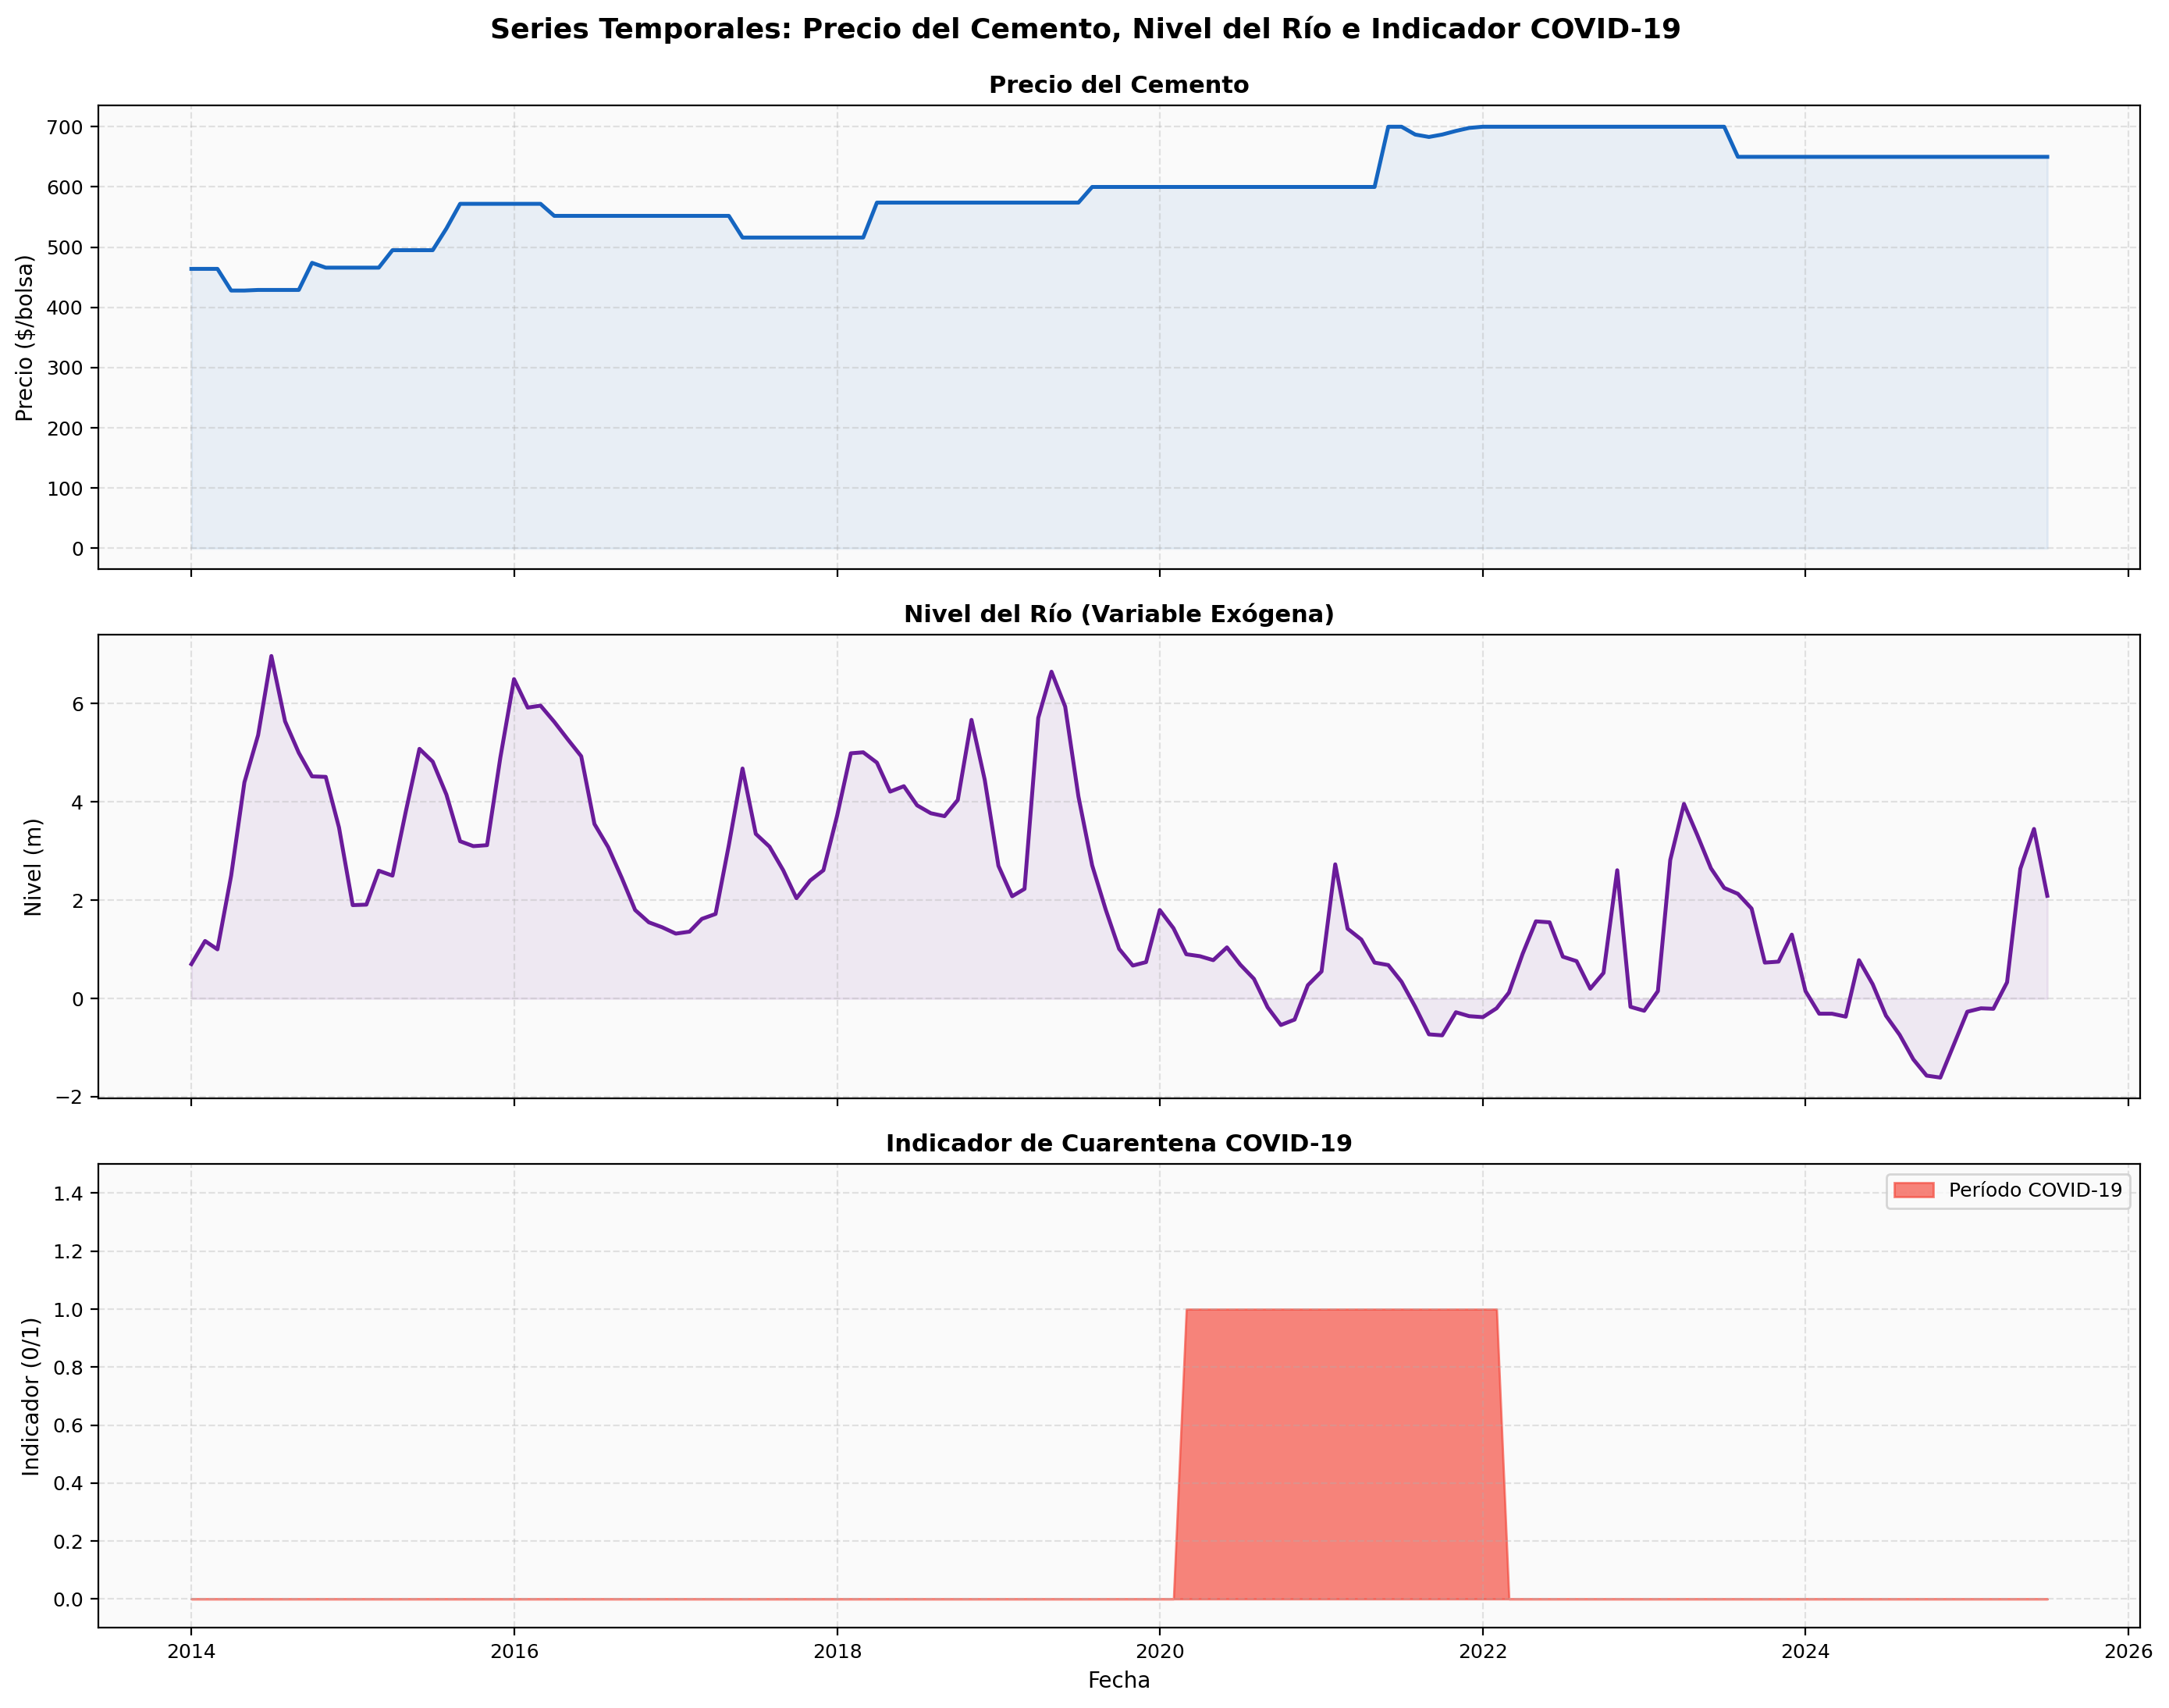
\includegraphics[width=\textwidth]{predicciones/prediccion_sarimax_ladrillo/graficos/01_series_temporales.png}
    \caption{Series temporales del precio mensual del ladrillo (Gs.) y del nivel del río Paraguay (m), período 2014--2025.}
    \label{fig:sarimax_ladrillo_series}
\end{figure}

\justify
La Figura \ref{fig:sarimax_ladrillo_series} muestra la evolución conjunta del precio del ladrillo y del nivel del río Paraguay. Se observa una tendencia ascendente en el precio del ladrillo a lo largo del período analizado, con incrementos escalonados que reflejan los ajustes de precio característicos de este mercado. El precio pasó de aproximadamente Gs.~428 en los primeros años a Gs.~700 hacia el final del período.

\begin{figure}[ht]
    \centering
    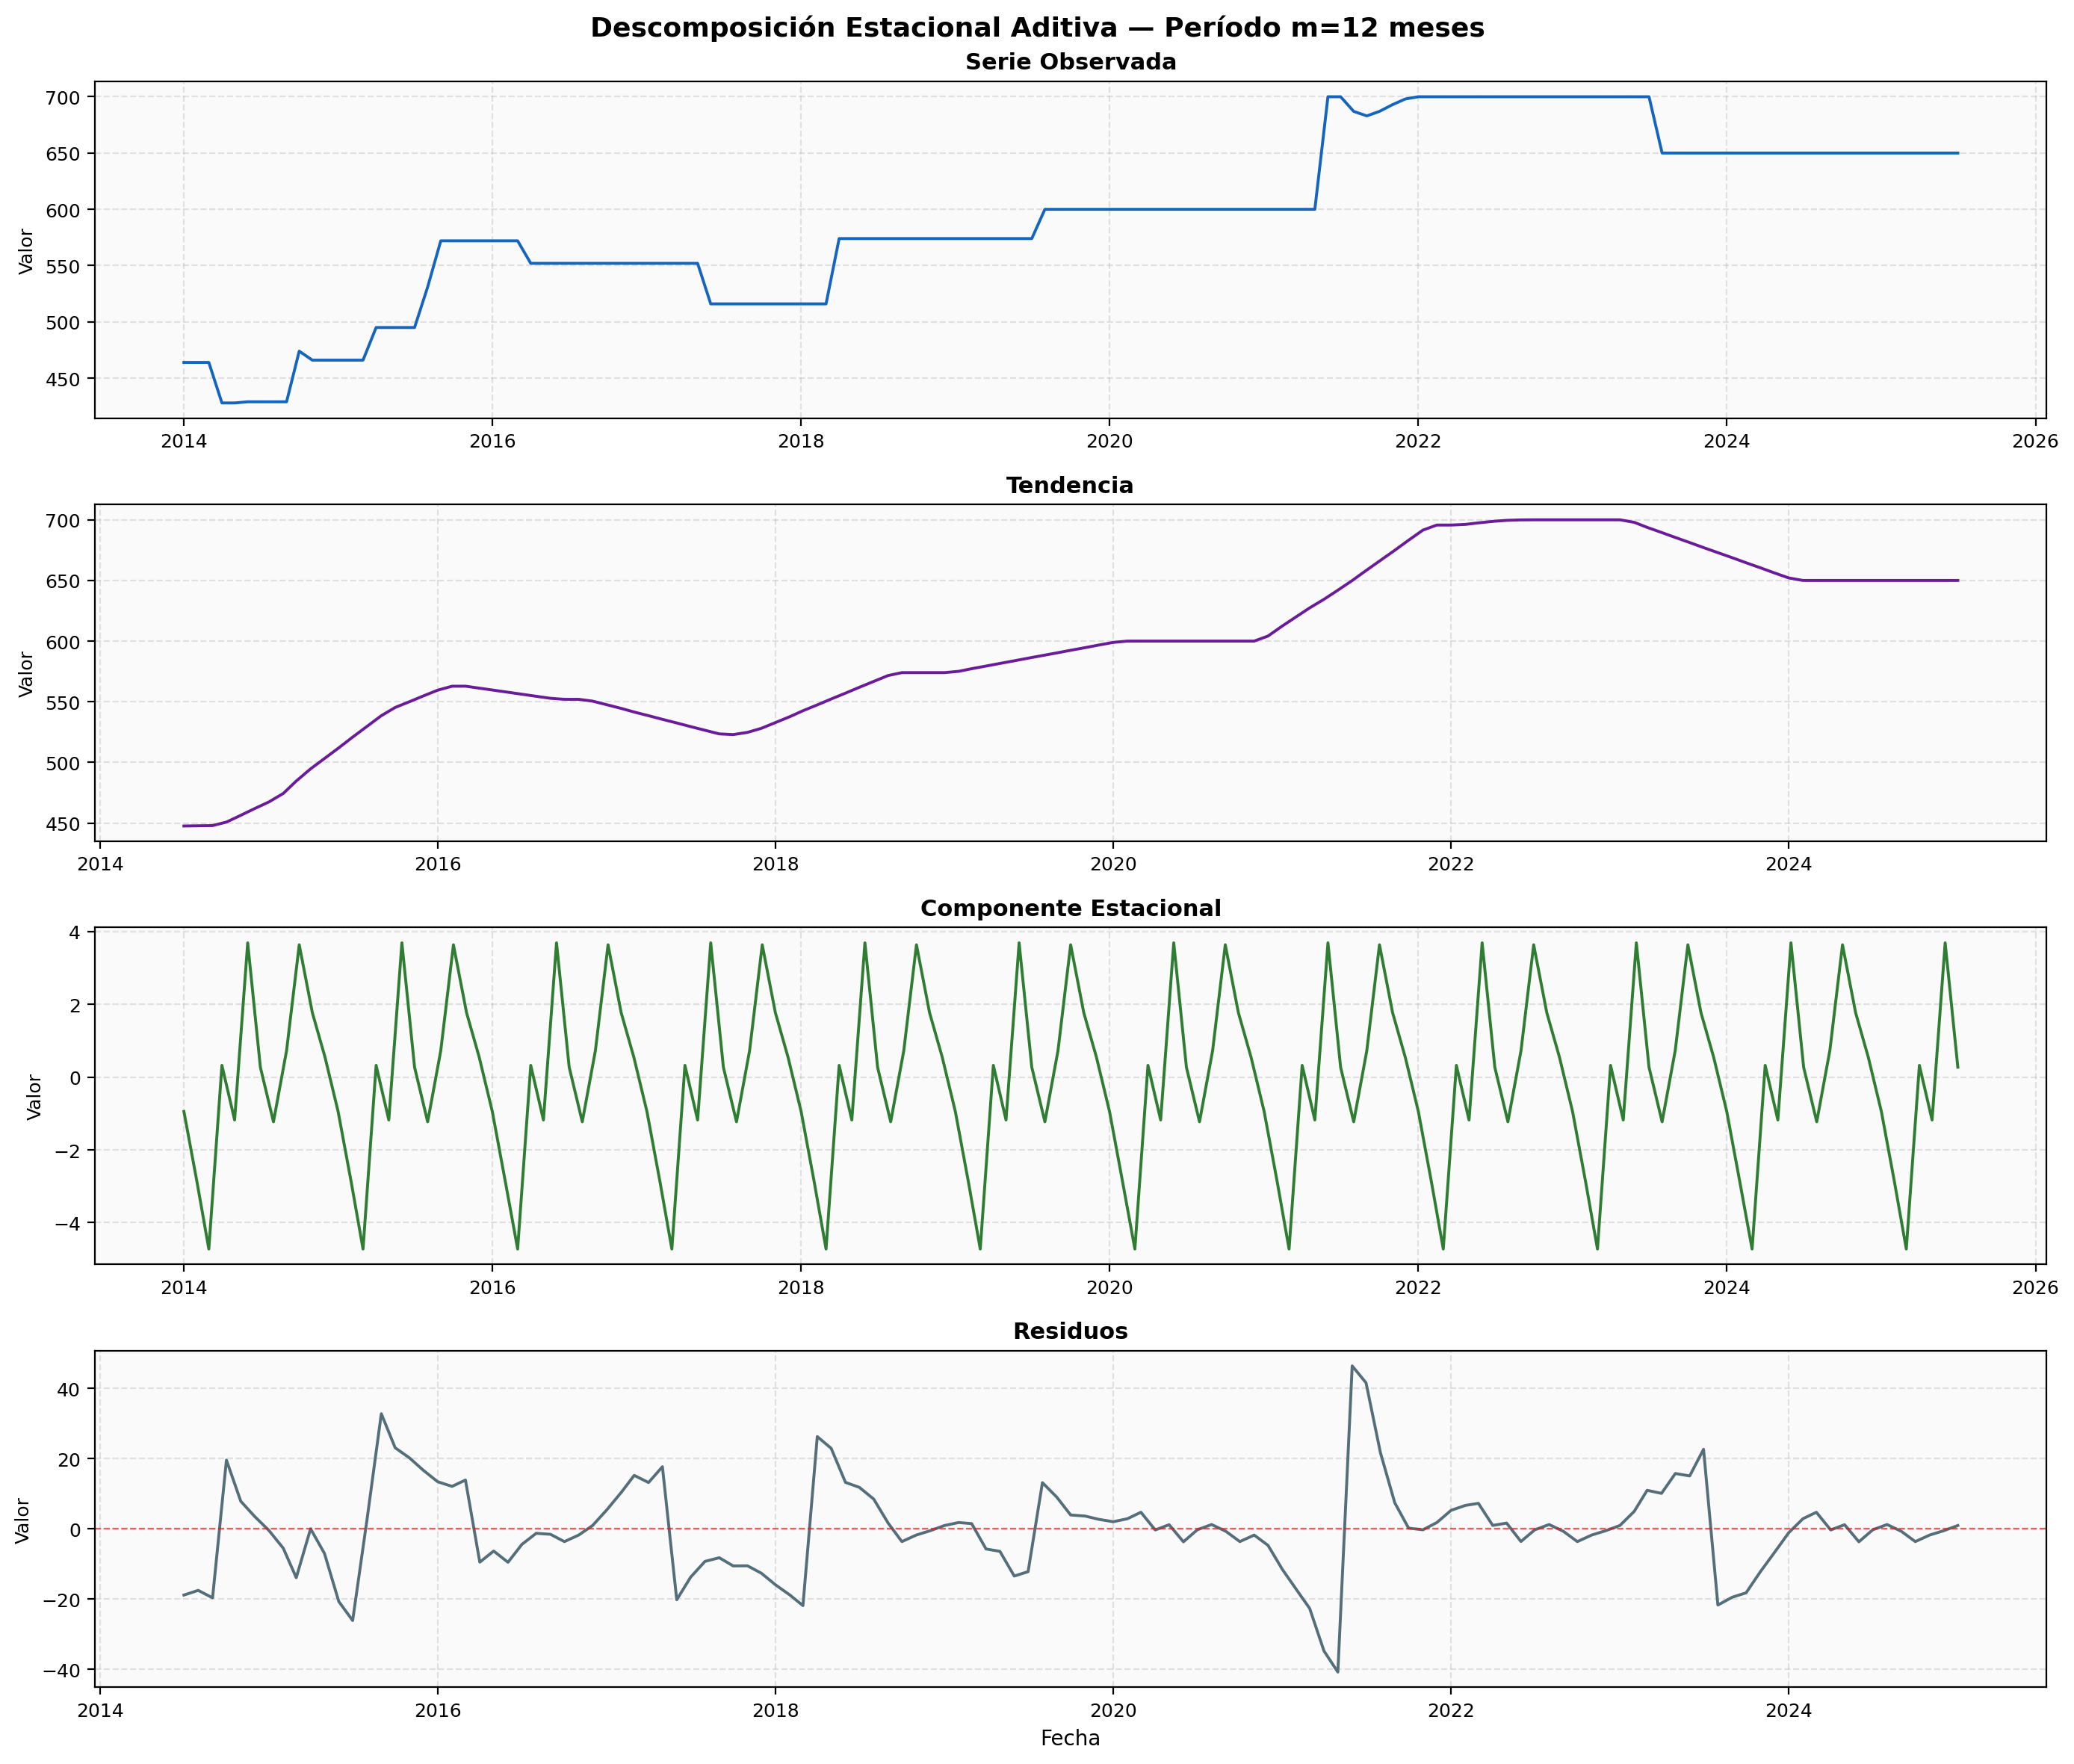
\includegraphics[width=\textwidth]{predicciones/prediccion_sarimax_ladrillo/graficos/02_descomposicion_estacional.png}
    \caption{Descomposición estacional de la serie de precio del ladrillo: tendencia, estacionalidad y componente residual.}
    \label{fig:sarimax_ladrillo_descomposicion}
\end{figure}

\justify
La Figura \ref{fig:sarimax_ladrillo_descomposicion} presenta la descomposición clásica de la serie del ladrillo. La componente de tendencia confirma el crecimiento sostenido del precio, con una aceleración a partir de 2020. La componente estacional muestra patrones de amplitud moderada con período anual, y los residuos no evidencian estructura sistemática.

\begin{figure}[ht]
    \centering
    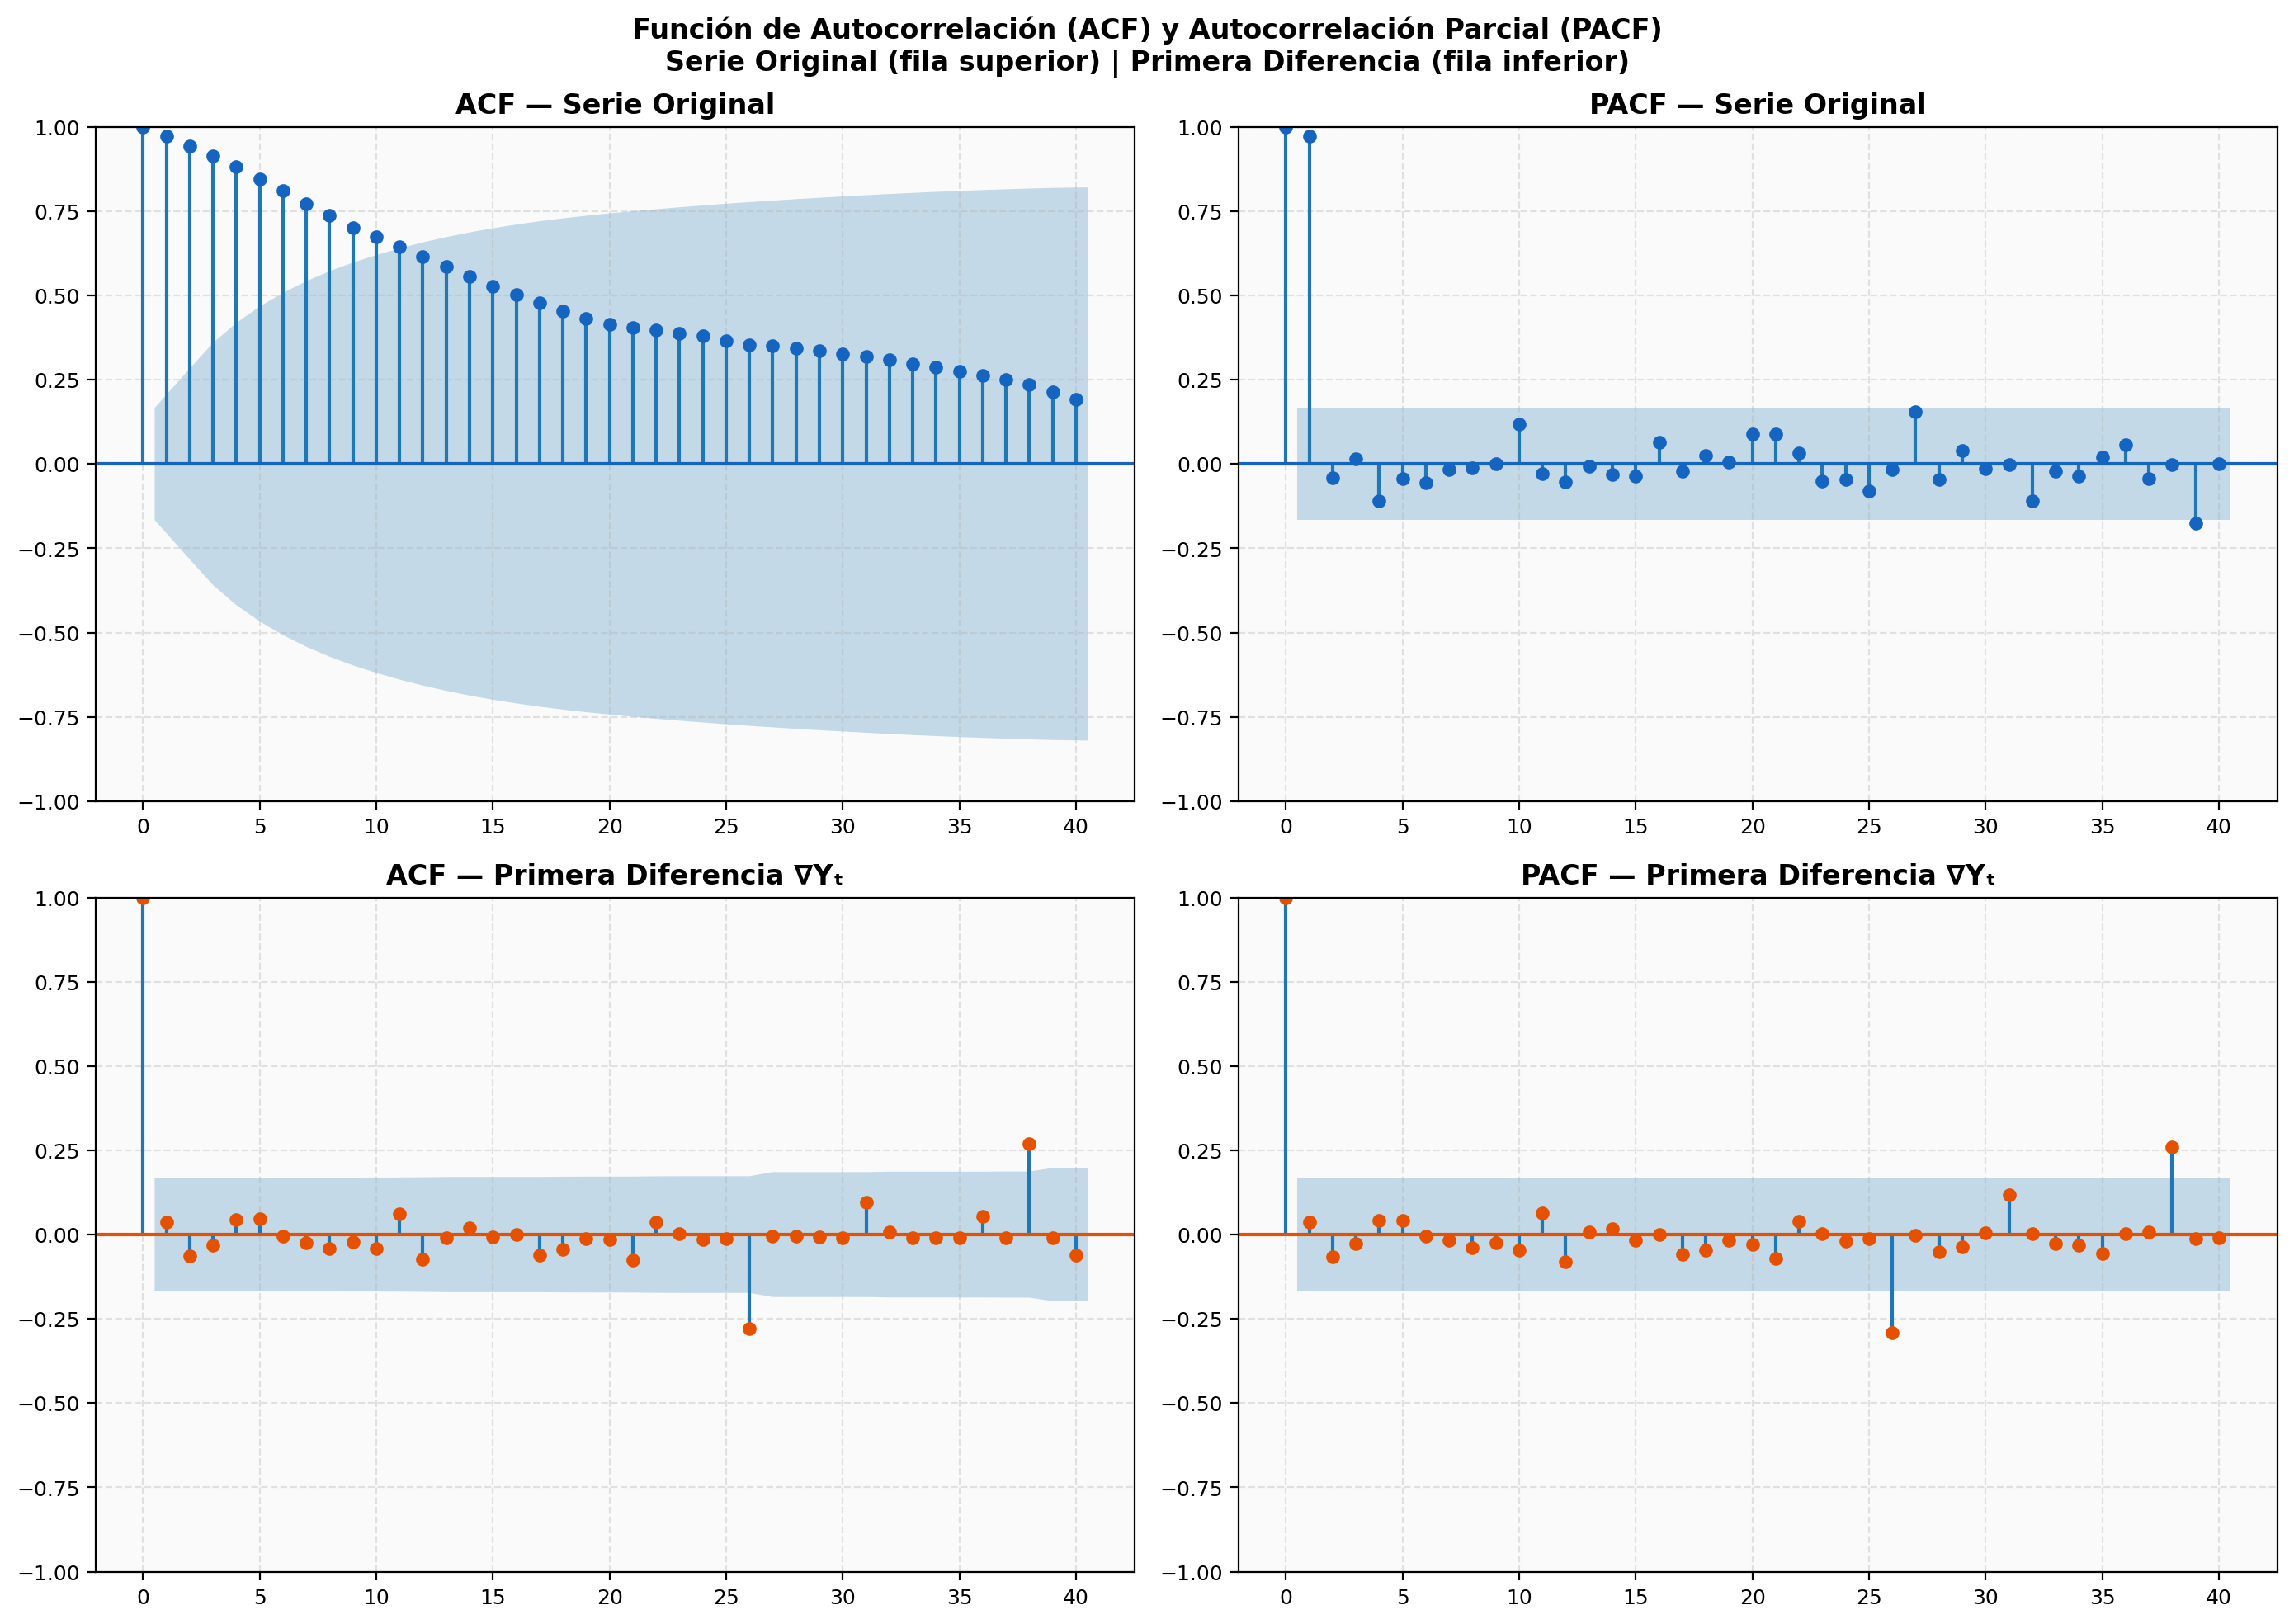
\includegraphics[width=\textwidth]{predicciones/prediccion_sarimax_ladrillo/graficos/03_acf_pacf.png}
    \caption{Funciones de autocorrelación (ACF) y autocorrelación parcial (PACF) de la serie del precio del ladrillo en niveles y en primeras diferencias.}
    \label{fig:sarimax_ladrillo_acf_pacf}
\end{figure}

\justify
La Figura \ref{fig:sarimax_ladrillo_acf_pacf} muestra las funciones ACF y PACF de la serie original y de su primera diferencia. Al igual que en el caso del cemento, la serie en niveles presenta una ACF con decaimiento lento, indicando no estacionariedad. Tras la primera diferencia, la ACF decae hacia cero, justificando el orden de integración $d=1$.

\begin{figure}[ht]
    \centering
    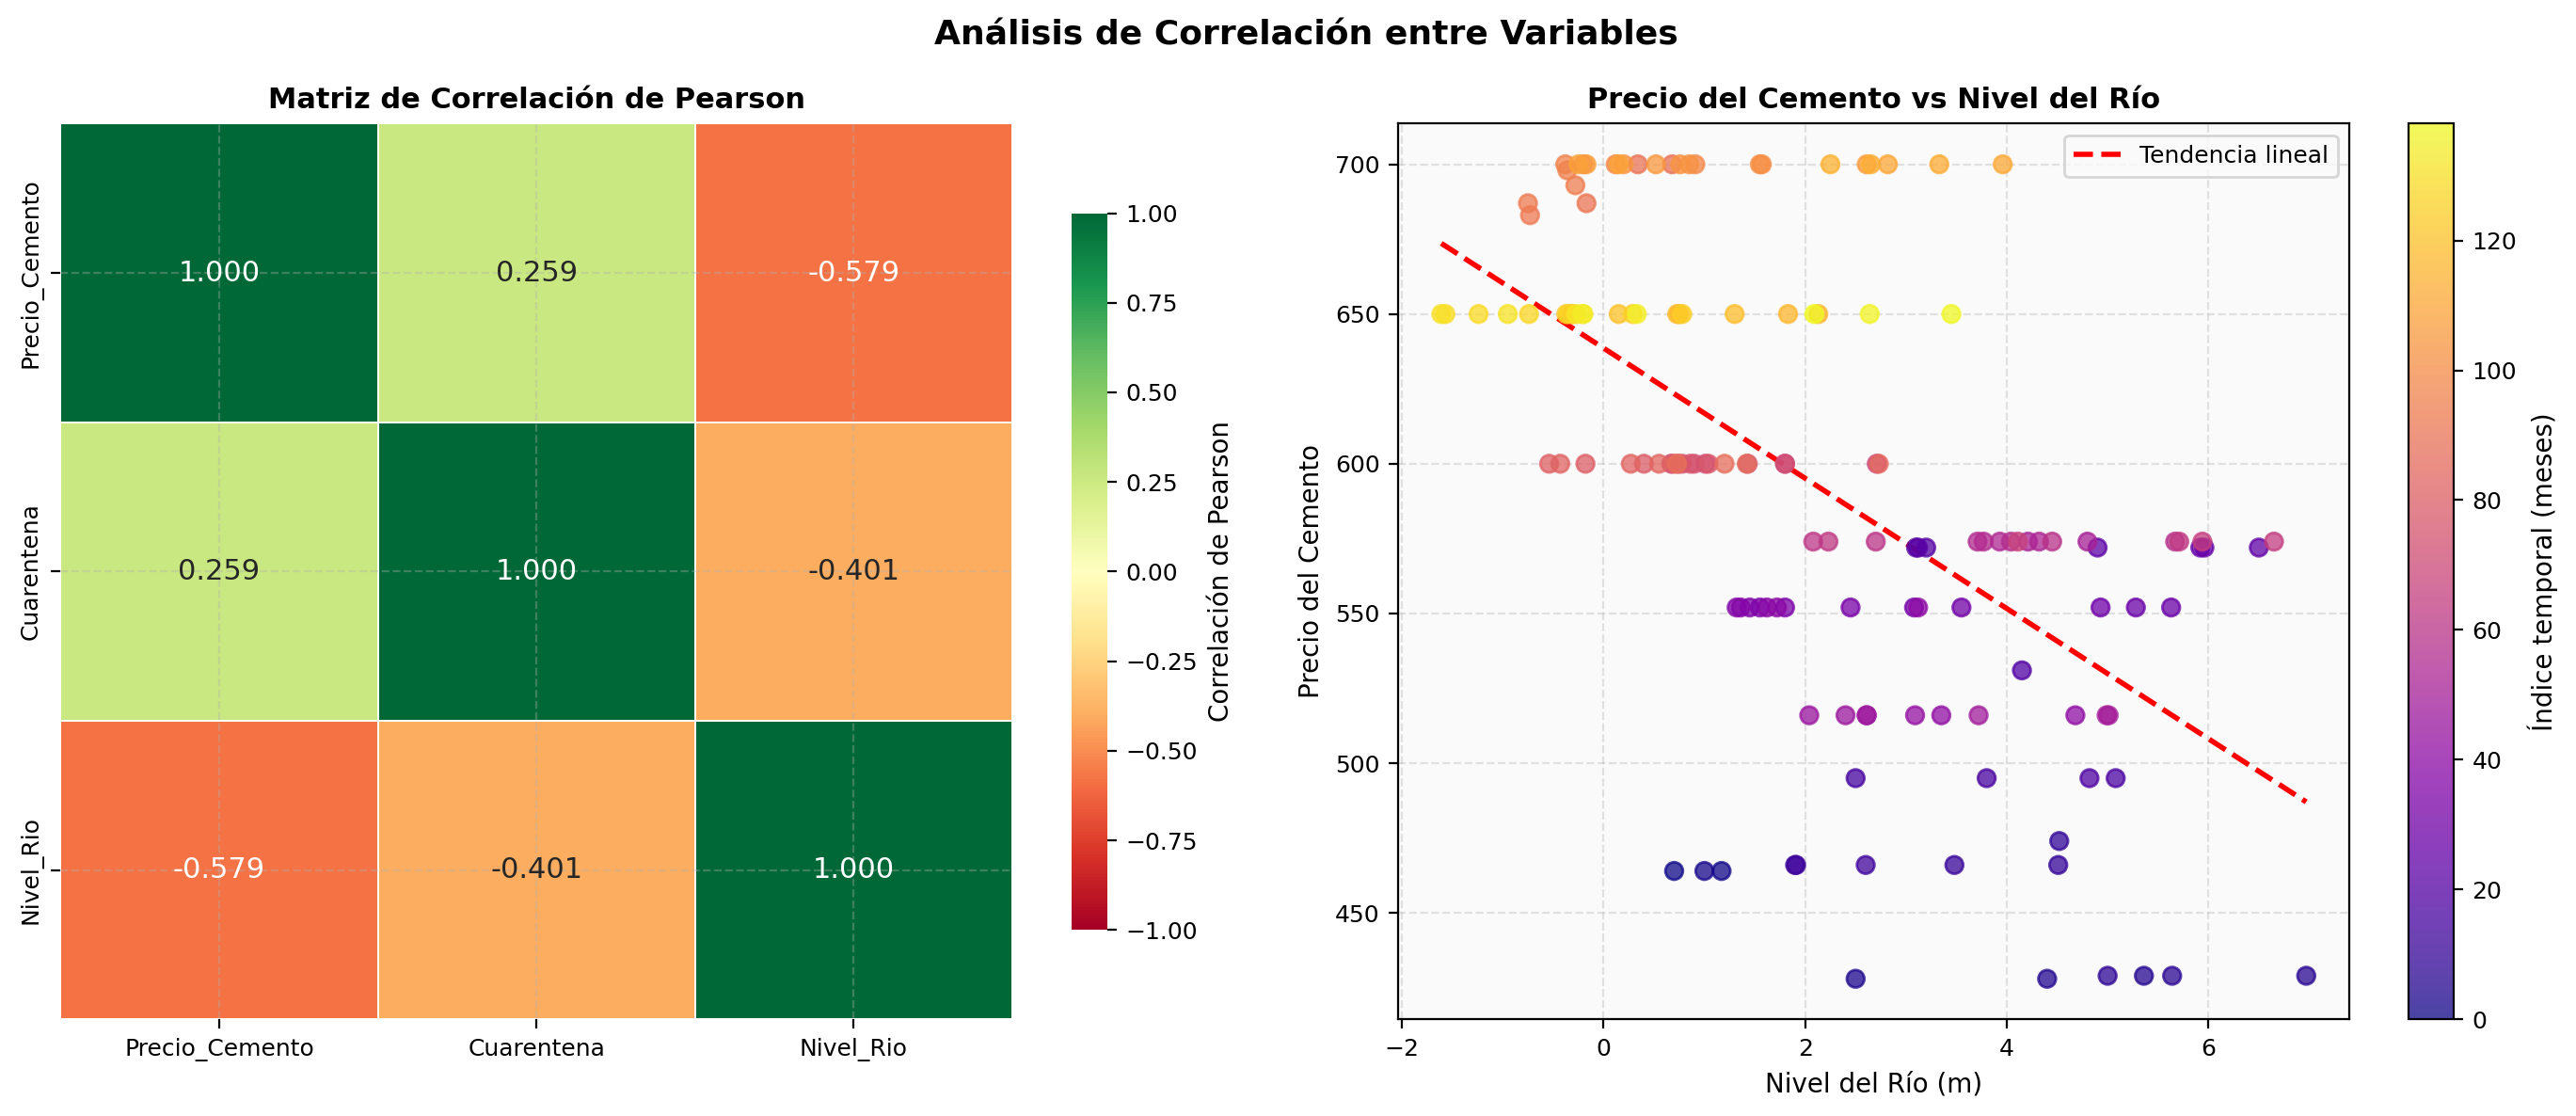
\includegraphics[width=0.8\textwidth]{predicciones/prediccion_sarimax_ladrillo/graficos/04_correlacion.png}
    \caption{Matriz de correlación entre el precio del ladrillo, el nivel del río Paraguay y la variable de cuarentena.}
    \label{fig:sarimax_ladrillo_correlacion}
\end{figure}

\justify
La Figura \ref{fig:sarimax_ladrillo_correlacion} muestra la matriz de correlación entre las variables del modelo. La correlación entre el precio del ladrillo y el nivel del río es de magnitud moderada y negativa, coherente con los resultados obtenidos para el cemento y con la hipótesis logística que sustenta la inclusión de esta variable exógena.

\begin{figure}[ht]
    \centering
    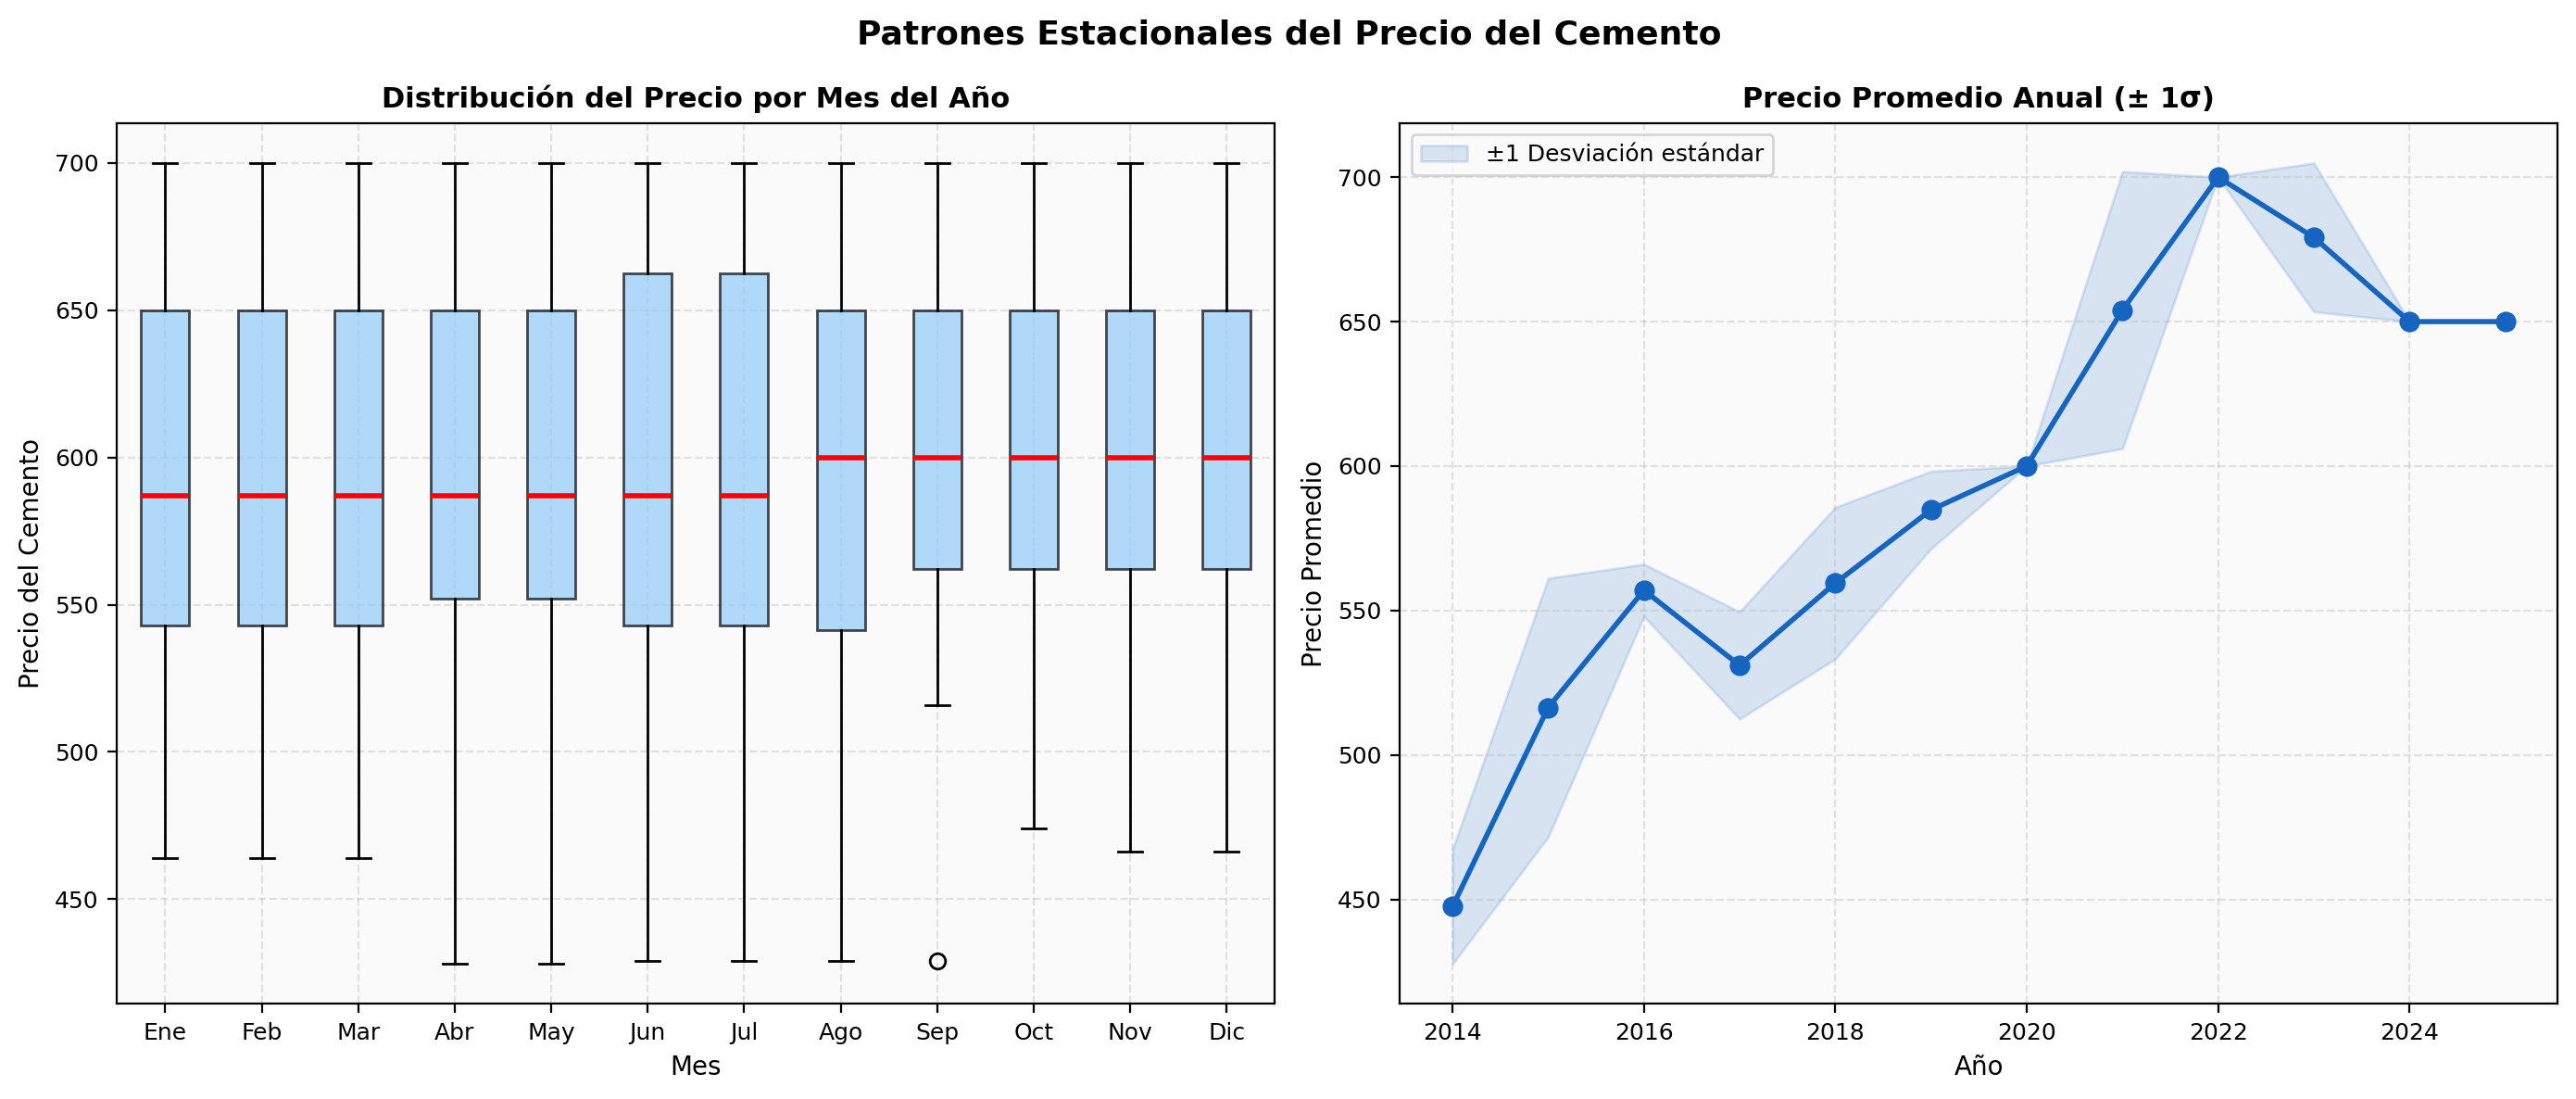
\includegraphics[width=\textwidth]{predicciones/prediccion_sarimax_ladrillo/graficos/05_patron_estacional.png}
    \caption{Patrón estacional del precio mensual del ladrillo a lo largo del año.}
    \label{fig:sarimax_ladrillo_estacional}
\end{figure}

\justify
La Figura \ref{fig:sarimax_ladrillo_estacional} ilustra el patrón estacional del precio del ladrillo. Se observan variaciones de amplitud moderada, con precios ligeramente superiores en los meses de mayor demanda de la construcción.

\subsubsection{Modelo SARIMAX: Selección y Parámetros}

\justify
La selección del orden óptimo del modelo SARIMAX se realizó mediante búsqueda exhaustiva sobre el espacio de parámetros $(p, d, q) \times (P, D, Q)_{12}$, minimizando el AIC. El modelo seleccionado corresponde al orden SARIMAX$(0,1,0)(0,0,0)_{12}$, coincidiendo con el resultado obtenido para el cemento, con un AIC de 1109{,}56 y un BIC de 1118{,}32.

\justify
Los parámetros estimados del modelo se resumen en la Tabla \ref{tab:sarimax_ladrillo_params}. El coeficiente asociado al nivel del río (\texttt{Nivel\_Rio}) resultó negativo ($-1{,}93$~Gs./m) y estadísticamente no significativo ($p=0{,}302$). La variable \texttt{Cuarentena} tampoco alcanzó significancia estadística ($p=0{,}999$), comportamiento análogo al observado en el modelo del cemento.

\begin{table}[ht]
    \centering
    \caption{Parámetros estimados del modelo SARIMAX$(0,1,0)(0,0,0)_{12}$ para la predicción del precio del ladrillo.}
    \label{tab:sarimax_ladrillo_params}
    \begin{tabular}{lrrrr}
        \toprule
        \textbf{Parámetro} & \textbf{Coeficiente} & \textbf{Error est.} & \textbf{z} & \textbf{p-valor} \\
        \midrule
        \texttt{Nivel\_Rio}  & $-1{,}931$ & $1{,}873$ & $-1{,}031$ & $0{,}302$ \\
        \texttt{Cuarentena}  & $-0{,}819$ & $643{,}258$ & $-0{,}001$ & $0{,}999$ \\
        $\sigma^{2}$         & $184{,}44$ & $6{,}384$ & $28{,}890$ & $0{,}000$ \\
        \midrule
        \multicolumn{2}{l}{AIC} & \multicolumn{3}{r}{1109{,}56} \\
        \multicolumn{2}{l}{BIC} & \multicolumn{3}{r}{1118{,}32} \\
        \multicolumn{2}{l}{Log-verosimilitud} & \multicolumn{3}{r}{$-551{,}78$} \\
        \bottomrule
    \end{tabular}
\end{table}

\justify
La coincidencia en el orden del modelo seleccionado ---SARIMAX$(0,1,0)$ tanto para el cemento como para el ladrillo--- sugiere que ambas series de precios comparten una dinámica subyacente similar: en su forma diferenciada, se comportan como ruido blanco con contribución marginal de las variables exógenas. Este resultado es coherente con mercados de insumos de construcción en los que los ajustes de precio son infrecuentes y se mantienen estables durante períodos prolongados.

\subsubsection{Modelo SARIMAX: Ajuste y Evaluación}

\begin{figure}[ht]
    \centering
    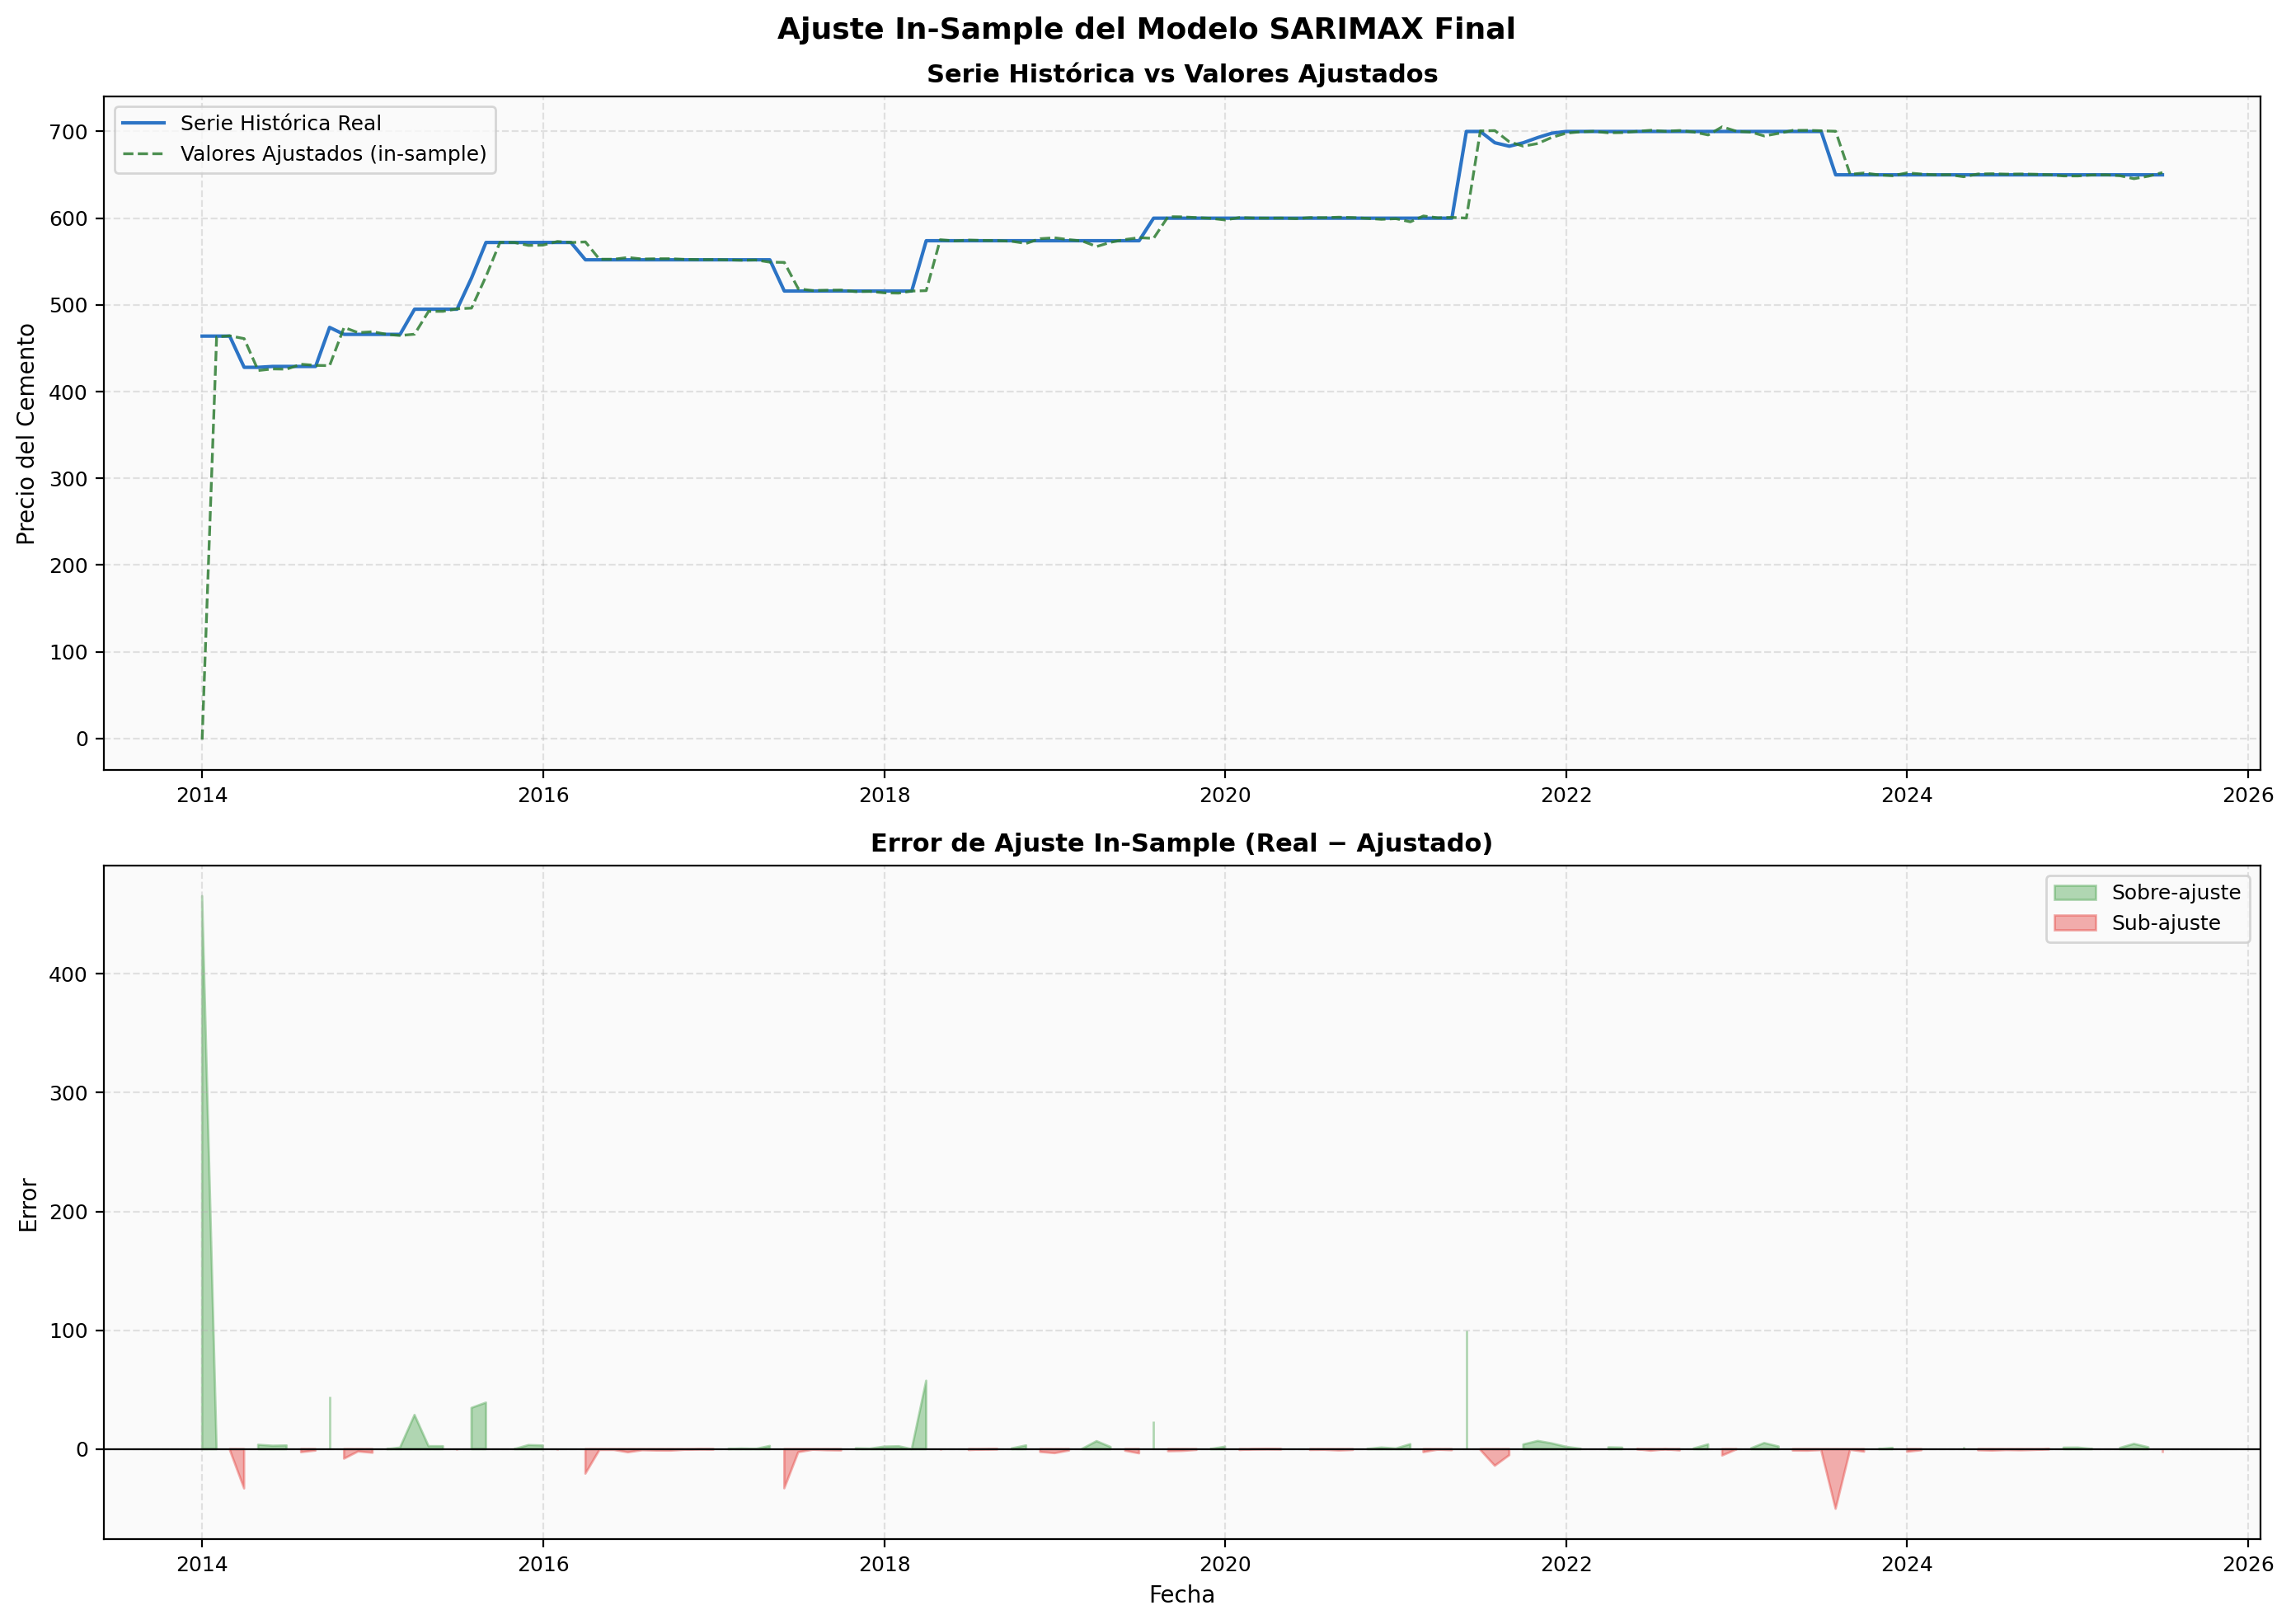
\includegraphics[width=\textwidth]{predicciones/prediccion_sarimax_ladrillo/graficos/11_ajuste_insample.png}
    \caption{Ajuste in-sample del modelo SARIMAX: valores reales versus valores ajustados para el precio del ladrillo.}
    \label{fig:sarimax_ladrillo_insample}
\end{figure}

\justify
La Figura \ref{fig:sarimax_ladrillo_insample} muestra el ajuste del modelo sobre los datos de entrenamiento. El modelo sigue adecuadamente la trayectoria histórica del precio del ladrillo, incluyendo los incrementos escalonados registrados a lo largo del período.

\begin{figure}[ht]
    \centering
    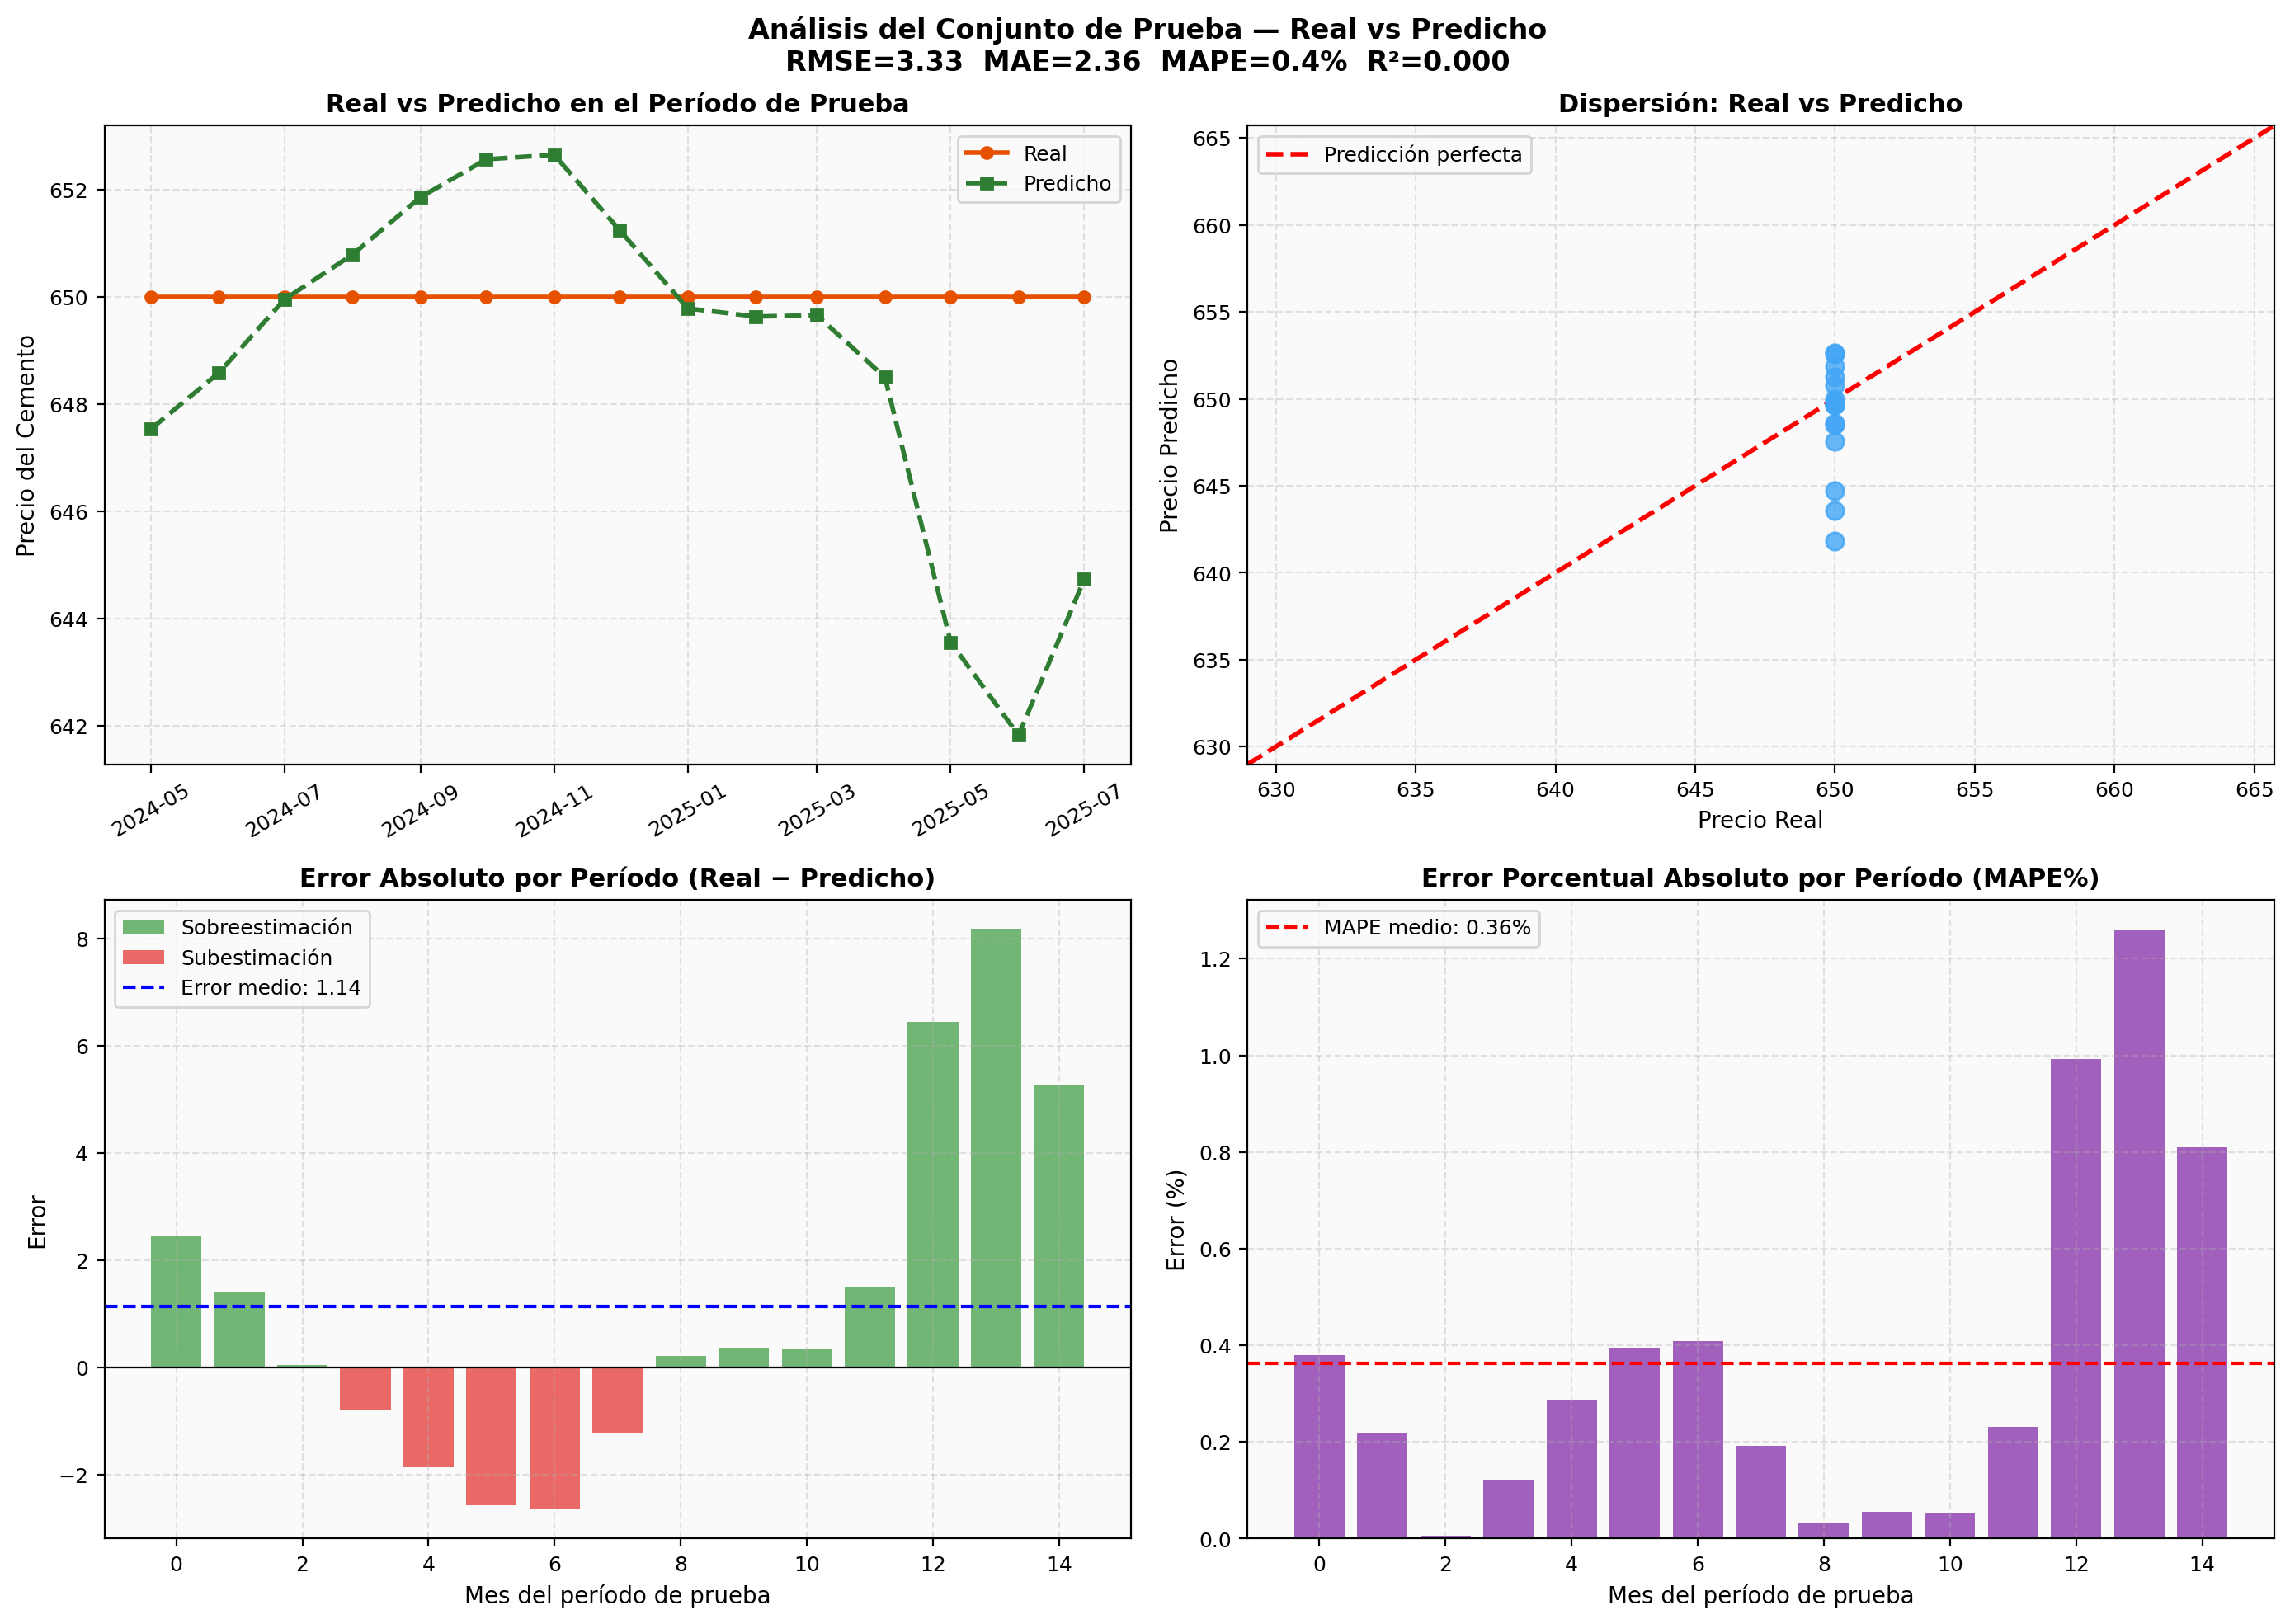
\includegraphics[width=\textwidth]{predicciones/prediccion_sarimax_ladrillo/graficos/08_comparacion_real_predicho.png}
    \caption{Comparación entre los valores reales y predichos del precio del ladrillo en el conjunto de prueba (15 meses).}
    \label{fig:sarimax_ladrillo_comparacion}
\end{figure}

\justify
La Figura \ref{fig:sarimax_ladrillo_comparacion} presenta la comparación entre los valores reales y los predichos por el modelo sobre el conjunto de prueba de 15 meses. Las métricas de evaluación se resumen en la Tabla \ref{tab:sarimax_ladrillo_metricas_prueba}.

\begin{table}[ht]
    \centering
    \caption{Métricas de evaluación del modelo SARIMAX sobre el conjunto de prueba del ladrillo (15 meses).}
    \label{tab:sarimax_ladrillo_metricas_prueba}
    \begin{tabular}{lc}
        \toprule
        \textbf{Métrica} & \textbf{Valor} \\
        \midrule
        RMSE (Raíz del Error Cuadrático Medio) & 3{,}33~Gs. \\
        MAE  (Error Absoluto Medio)            & 2{,}36~Gs. \\
        MAPE (Error Porcentual Medio Absoluto) & 0{,}36\,\% \\
        SMAPE (Error Porcentual Simétrico)     & 0{,}36\,\% \\
        Error Absoluto Máximo                  & 8{,}18~Gs. \\
        $R^{2}$ (Coeficiente de Determinación) & 0{,}0000 \\
        \bottomrule
    \end{tabular}
\end{table}

\justify
Al igual que en el caso del cemento, el MAPE de 0{,}36\,\% indica predicciones puntuales con un error relativo muy bajo, pero el $R^{2}=0$ refleja que durante el período de prueba el precio del ladrillo se mantuvo prácticamente estable, de modo que el modelo no puede diferenciarse de una predicción constante en términos de varianza explicada. El patrón es consistente con la naturaleza del modelo $(0,1,0)$: el pronóstico corresponde al último valor observado ajustado por las variables exógenas.

\subsubsection{Modelo SARIMAX: Validación Cruzada}

\begin{figure}[ht]
    \centering
    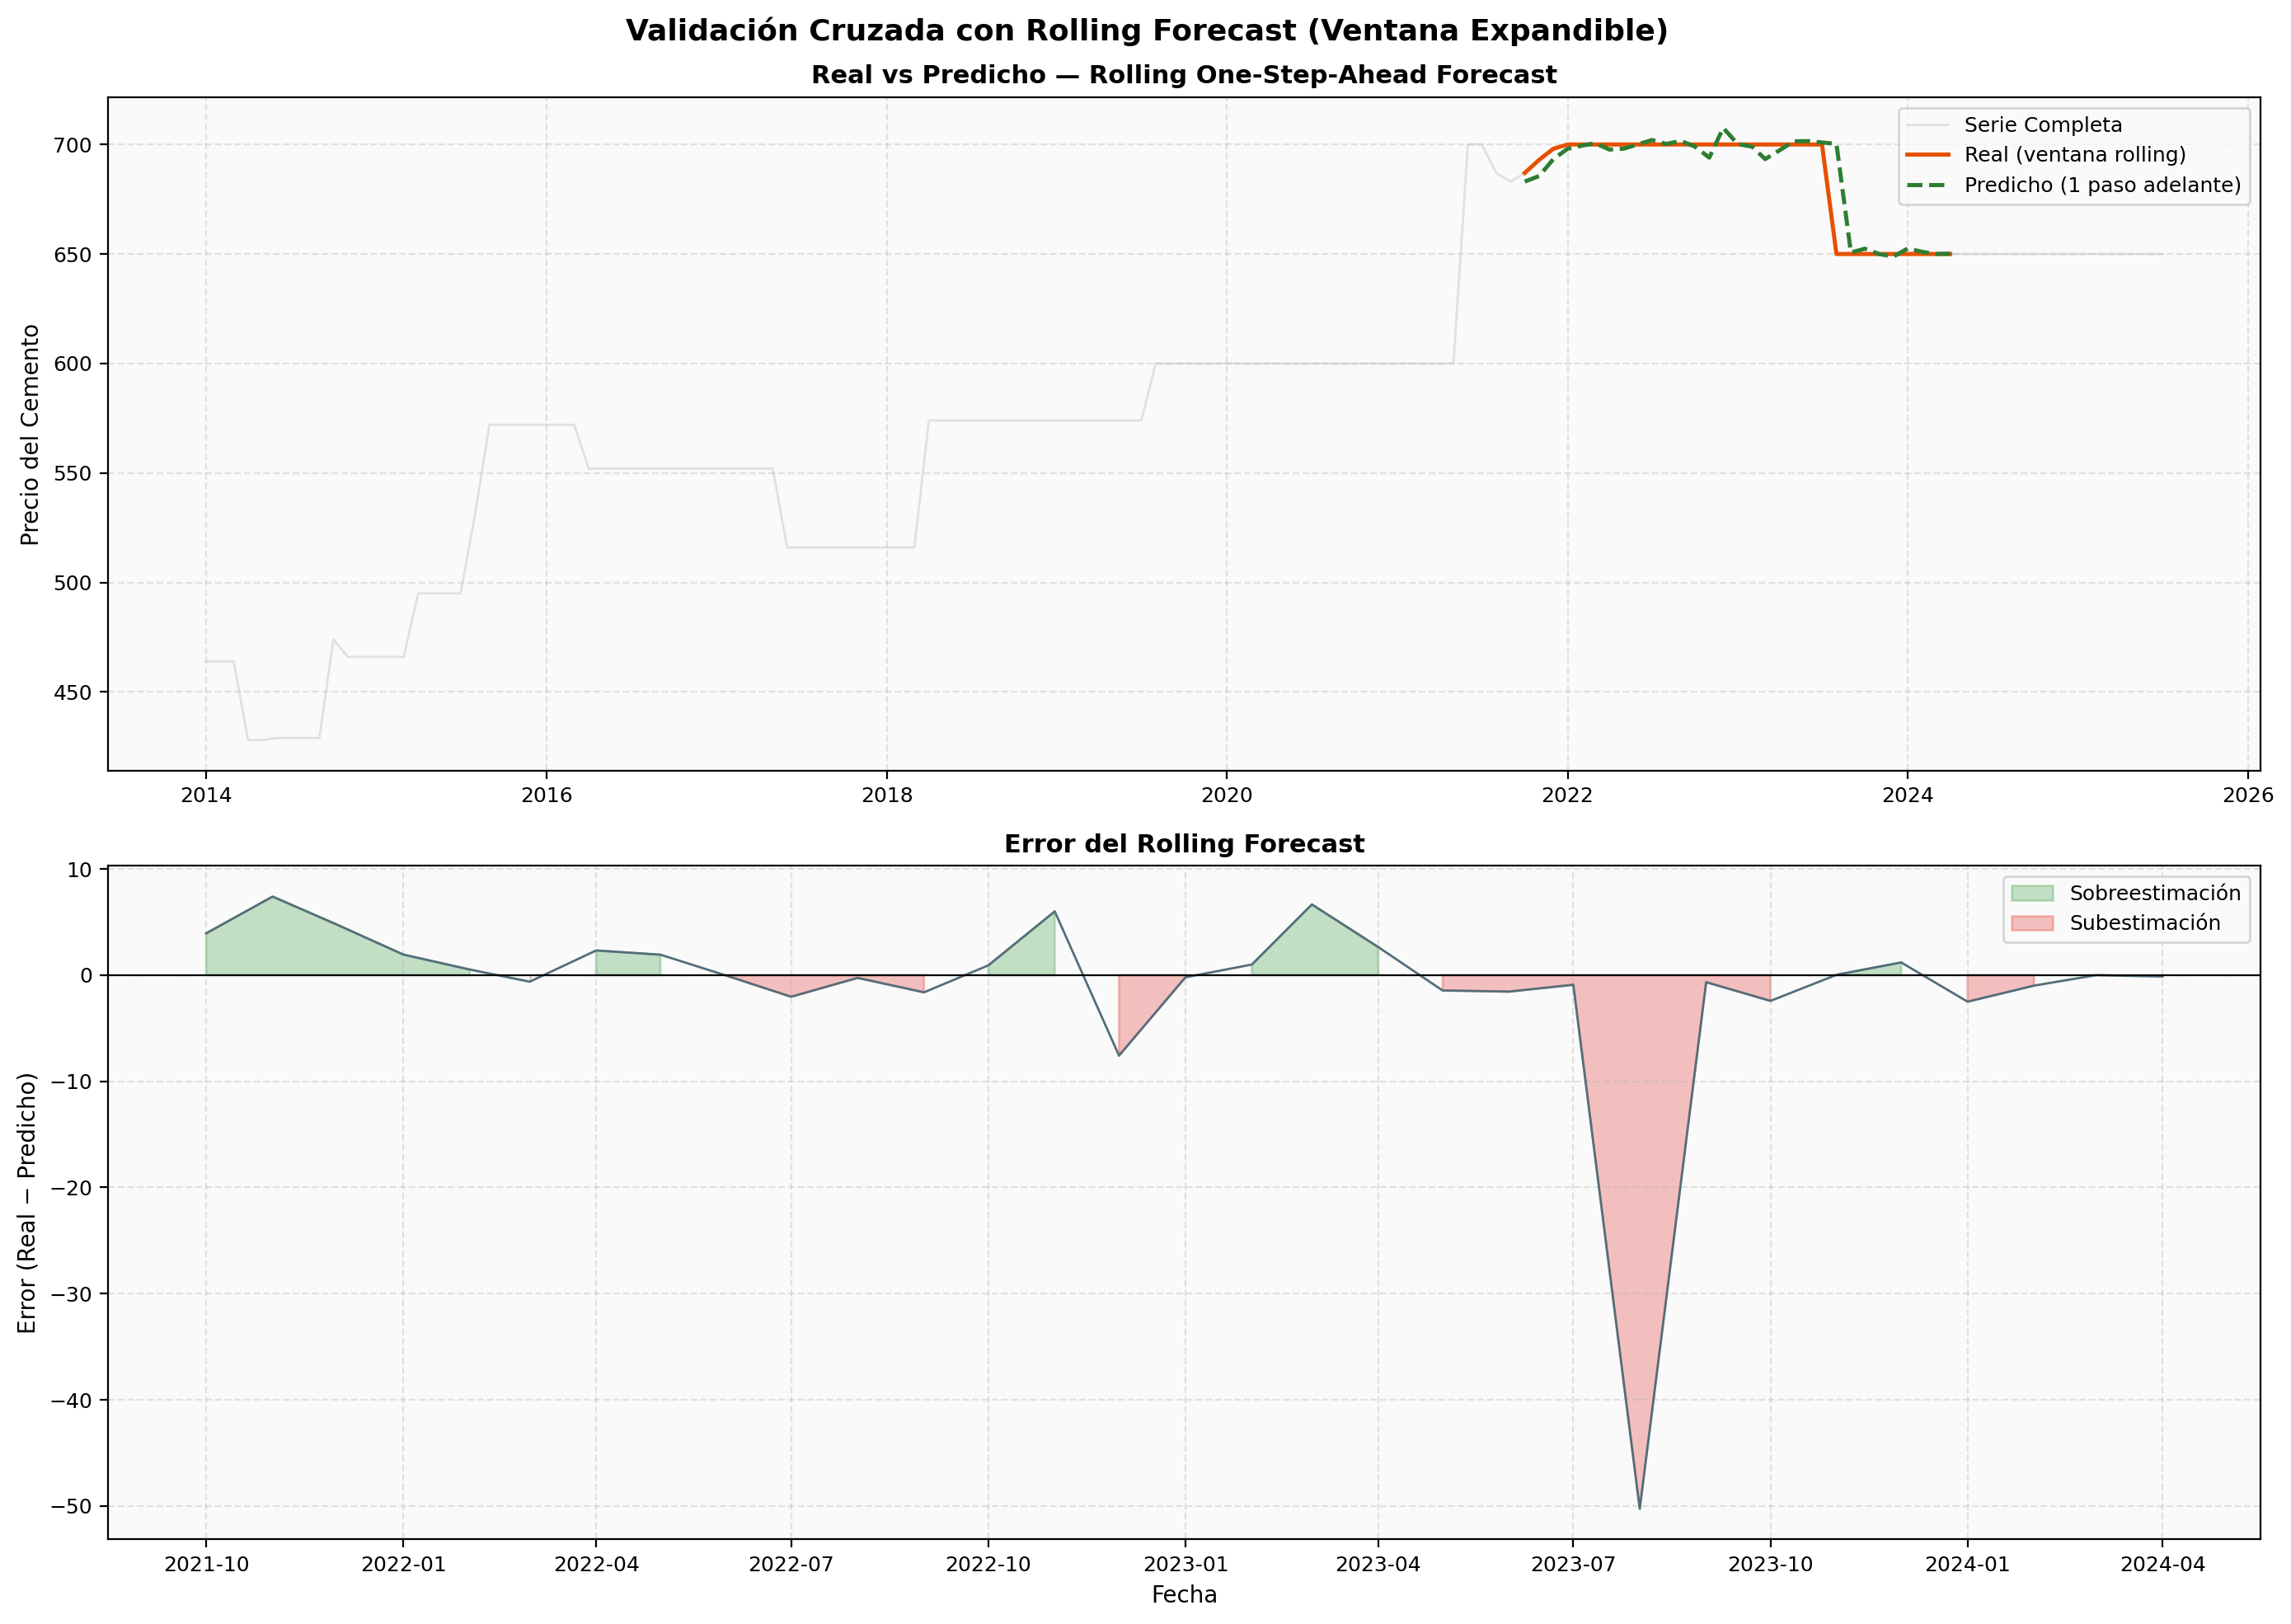
\includegraphics[width=\textwidth]{predicciones/prediccion_sarimax_ladrillo/graficos/10_rolling_forecast_cv.png}
    \caption{Validación cruzada por ventana deslizante del modelo SARIMAX para el precio del ladrillo.}
    \label{fig:sarimax_ladrillo_rolling}
\end{figure}

\justify
La validación cruzada por ventana deslizante ofrece un panorama más representativo del desempeño del modelo. La Figura \ref{fig:sarimax_ladrillo_rolling} muestra las predicciones un paso adelante a lo largo de todo el período evaluado. Las métricas obtenidas se presentan en la Tabla \ref{tab:sarimax_ladrillo_metricas_cv}.

\begin{table}[ht]
    \centering
    \caption{Métricas de validación cruzada por ventana deslizante del modelo SARIMAX para el ladrillo.}
    \label{tab:sarimax_ladrillo_metricas_cv}
    \begin{tabular}{lc}
        \toprule
        \textbf{Métrica} & \textbf{Valor} \\
        \midrule
        RMSE & 9{,}52~Gs. \\
        MAE  & 3{,}69~Gs. \\
        MAPE & 0{,}55\,\% \\
        $R^{2}$ & 0{,}8193 \\
        \bottomrule
    \end{tabular}
\end{table}

\justify
El $R^{2}=0{,}8193$ indica que el modelo explica el 81{,}93\,\% de la varianza del precio del ladrillo a lo largo del período histórico completo, superando incluso al resultado obtenido para el cemento ($R^{2}=0{,}7586$). El MAPE de 0{,}55\,\%, inferior al umbral del 5\,\% habitual para series de precios de materiales, confirma la utilidad práctica del modelo para la estimación presupuestaria.

\subsubsection{Modelo SARIMAX: Análisis de Residuos}

\begin{figure}[ht]
    \centering
    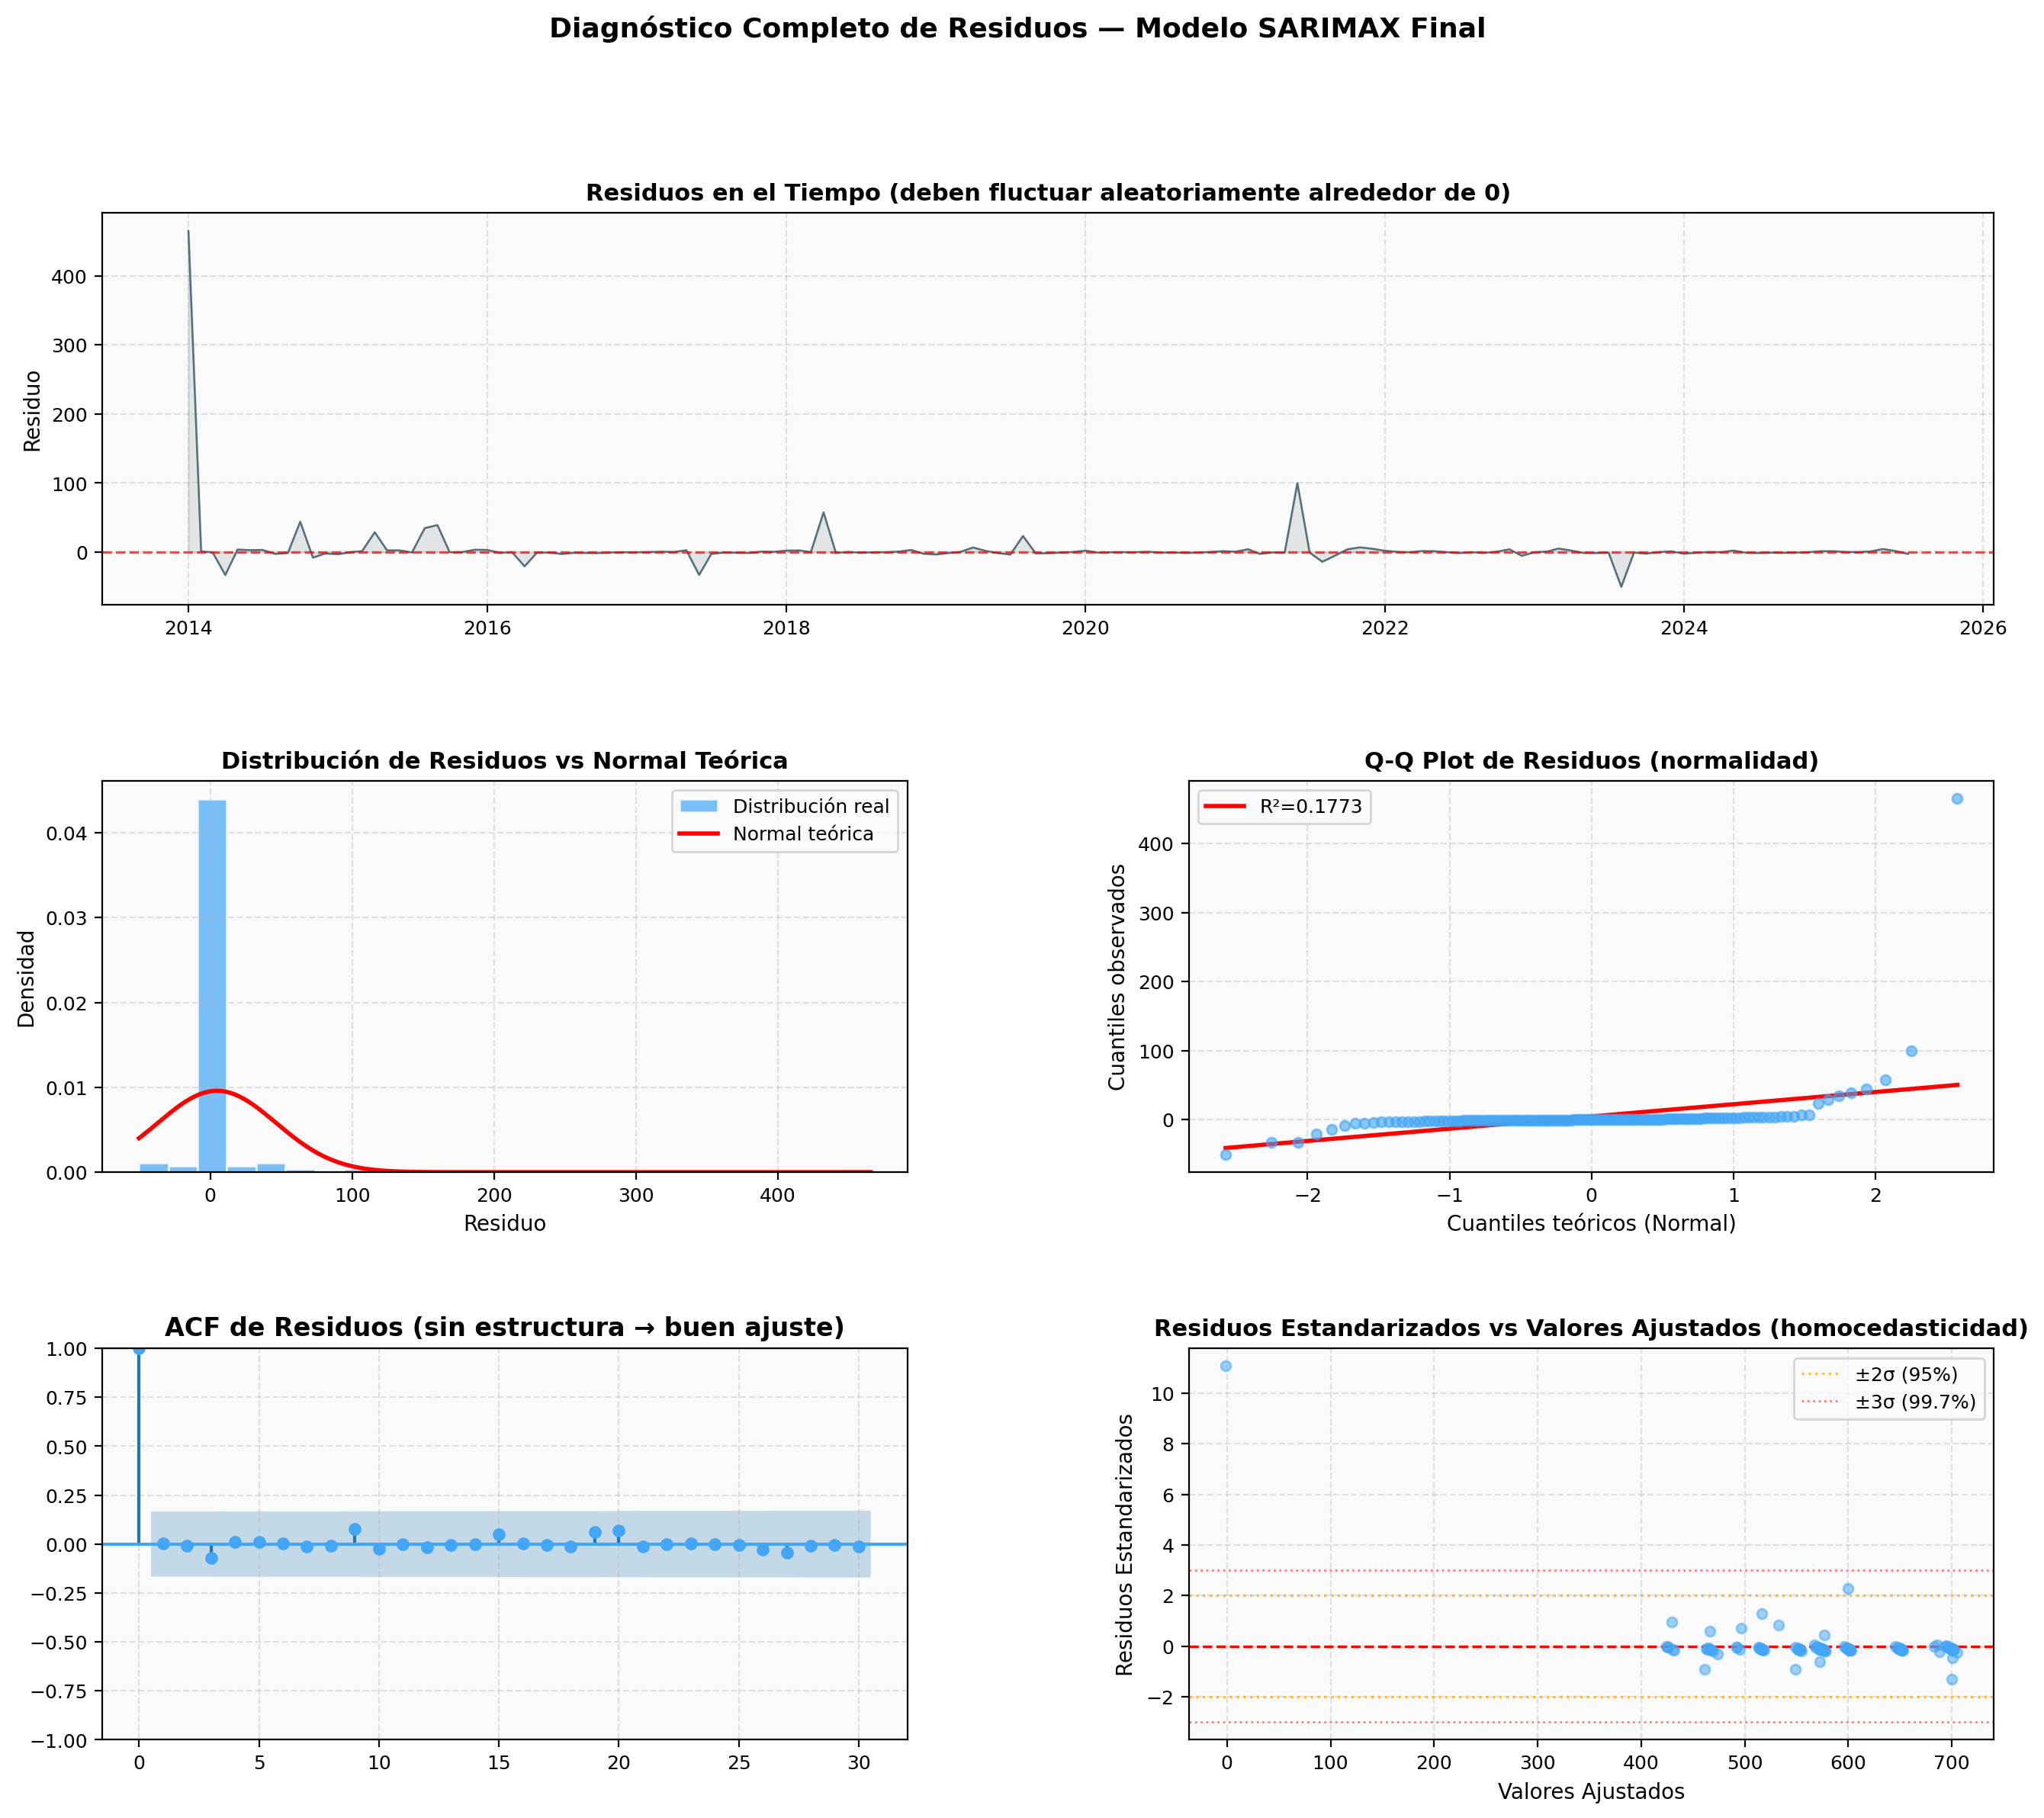
\includegraphics[width=\textwidth]{predicciones/prediccion_sarimax_ladrillo/graficos/07_diagnostico_residuos.png}
    \caption{Diagnóstico de residuos del modelo SARIMAX para el precio del ladrillo.}
    \label{fig:sarimax_ladrillo_residuos}
\end{figure}

\justify
La Figura \ref{fig:sarimax_ladrillo_residuos} presenta el diagnóstico de los residuos. El test de Ljung-Box no rechaza la hipótesis nula de ausencia de autocorrelación serial para los rezagos 10 ($Q=1{,}80$, $p=0{,}998$) y 20 ($Q=3{,}72$, $p=1{,}000$), confirmando que los residuos se comportan como ruido blanco. El test de Shapiro-Wilk rechaza la normalidad ($W=0{,}1936$, $p<0{,}001$), resultado atribuible a la presencia de observaciones extremas que introducen una curtosis de 26{,}69 y una asimetría de 3{,}25. Al igual que en el modelo del cemento, esta no normalidad no invalida las estimaciones puntuales pero impone cautela en la interpretación de los intervalos de confianza.

\subsubsection{Modelo SARIMAX: Pronóstico a 24 Meses}

\begin{figure}[ht]
    \centering
    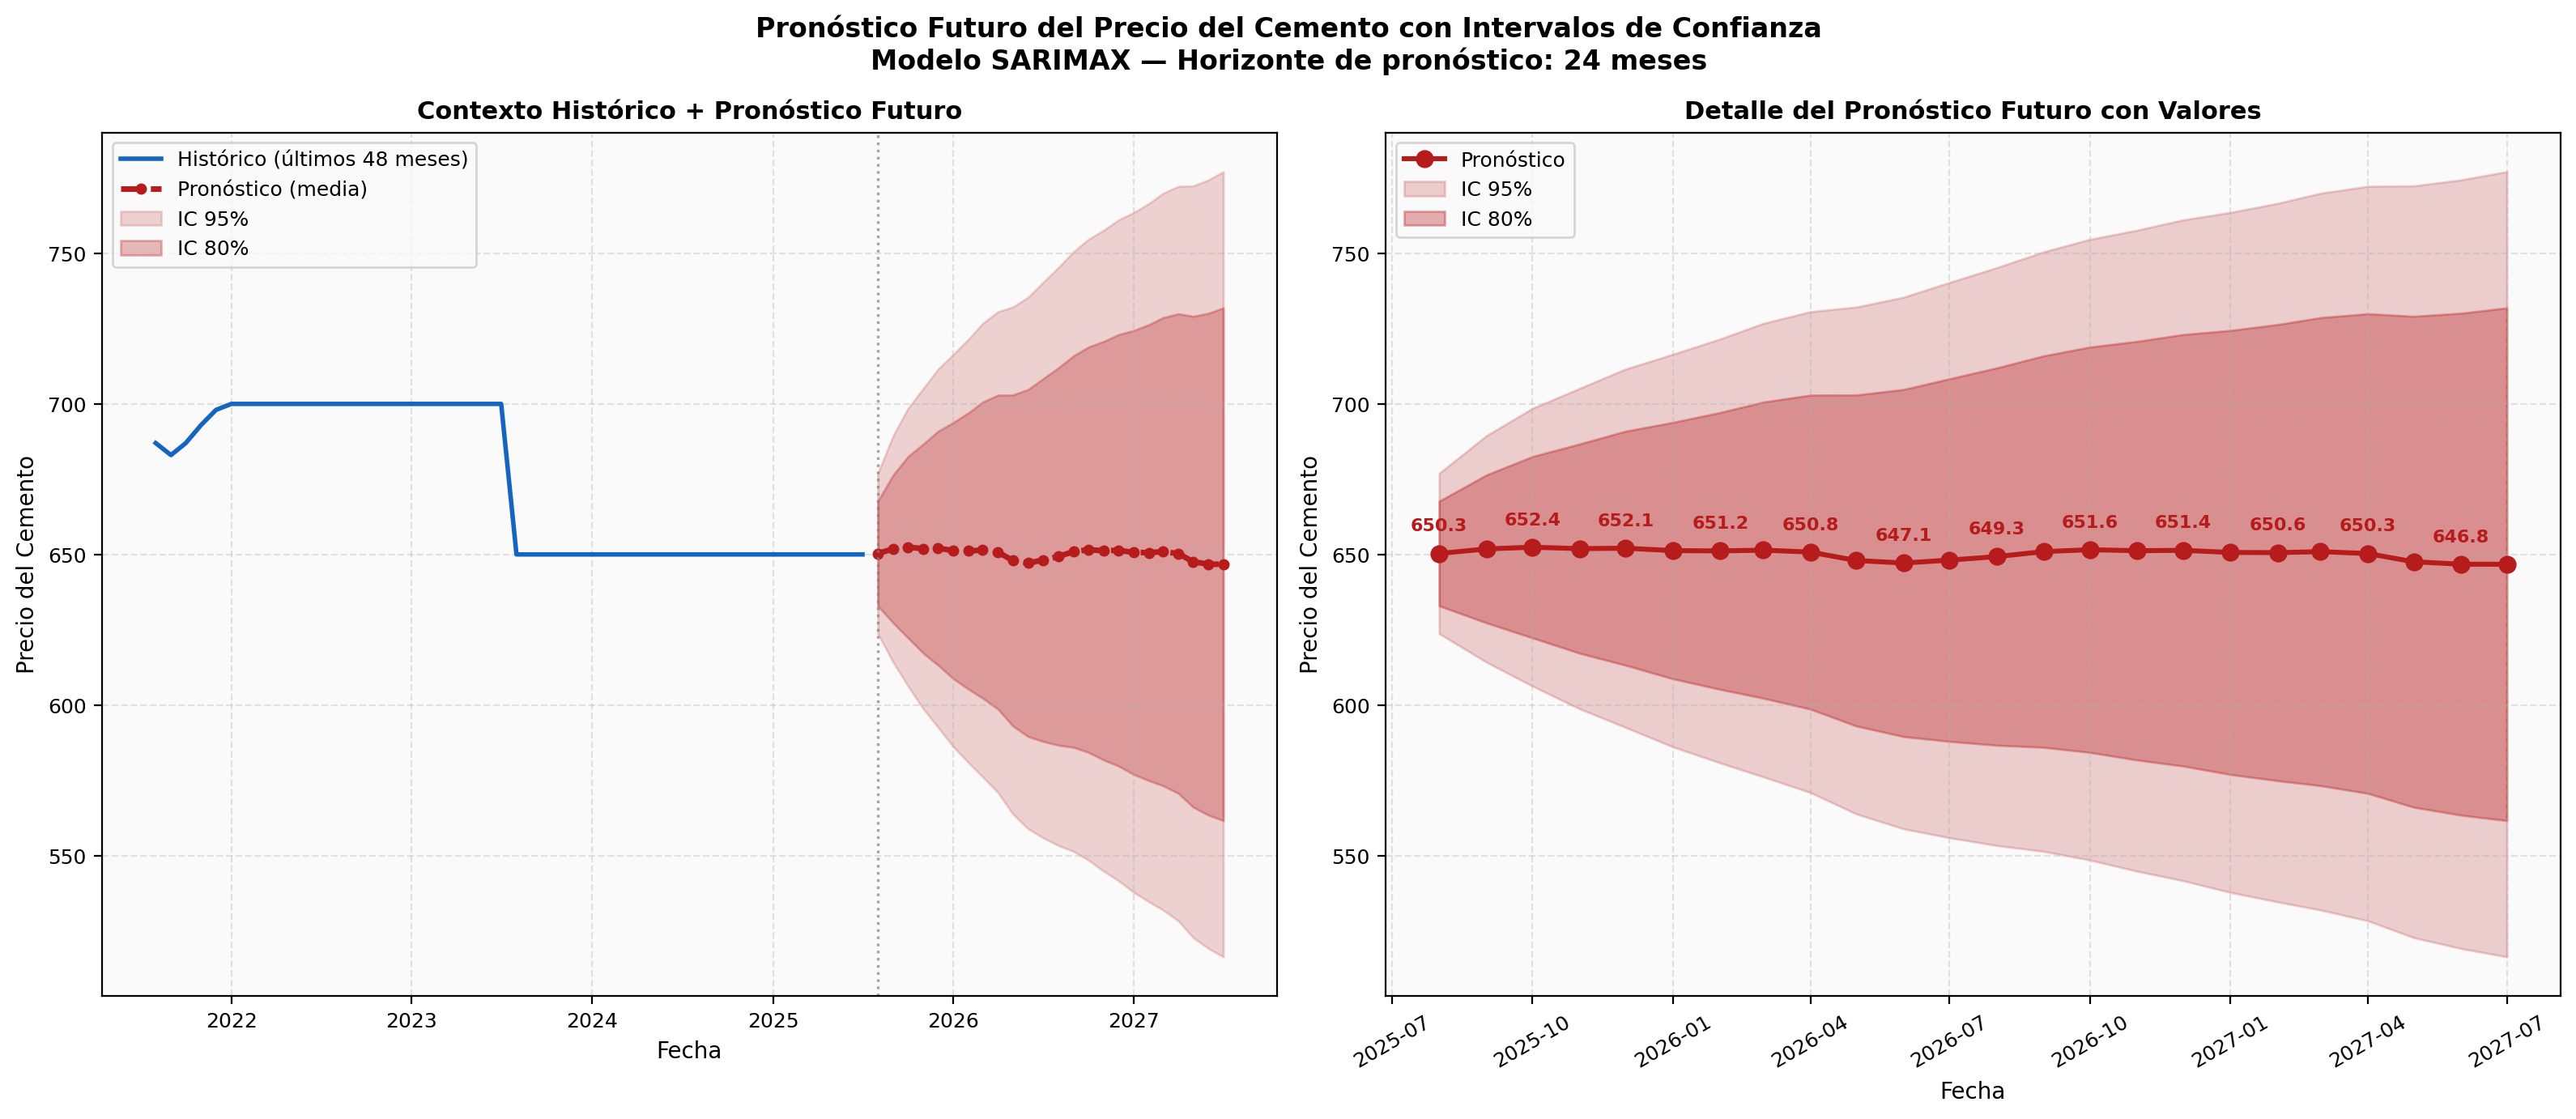
\includegraphics[width=\textwidth]{predicciones/prediccion_sarimax_ladrillo/graficos/09_pronostico_intervalo_confianza.png}
    \caption{Pronóstico del precio del ladrillo a 24 meses (agosto 2025 -- julio 2027) con intervalos de confianza al 95\,\%.}
    \label{fig:sarimax_ladrillo_pronostico_ic}
\end{figure}

\begin{figure}[ht]
    \centering
    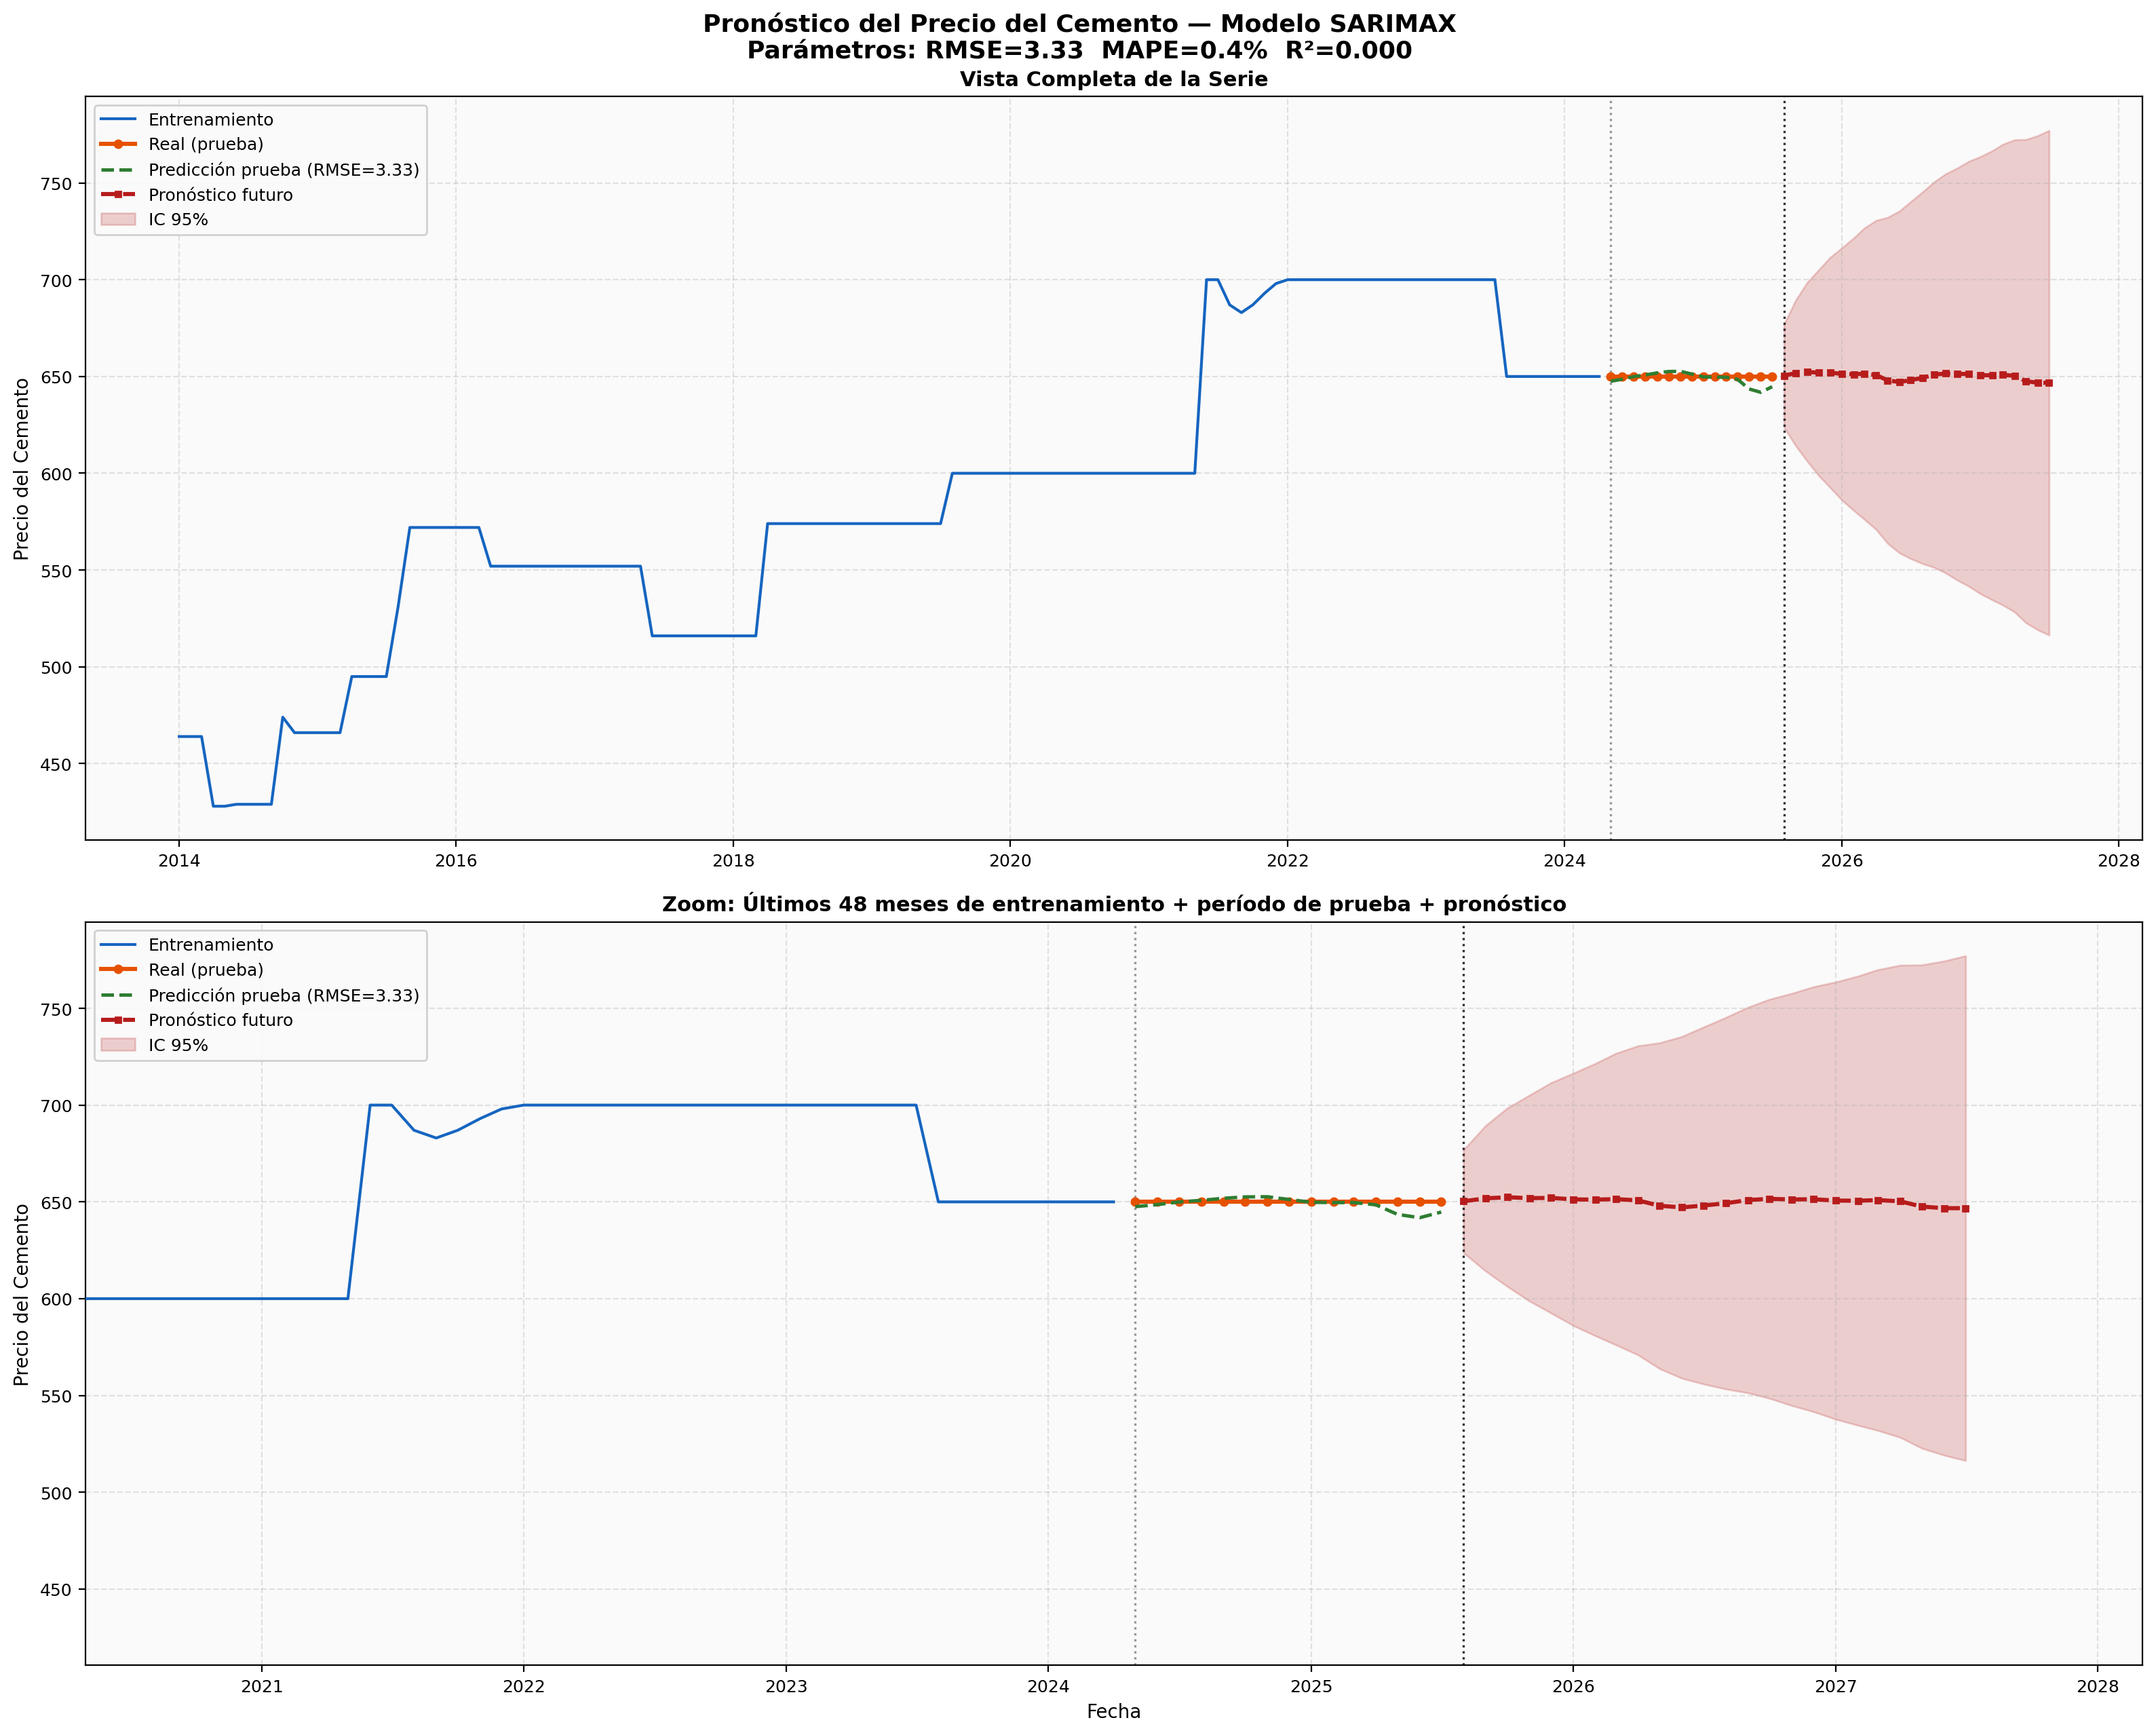
\includegraphics[width=\textwidth]{predicciones/prediccion_sarimax_ladrillo/graficos/06_pronostico_completo.png}
    \caption{Pronóstico completo del precio del ladrillo: serie histórica observada y proyección SARIMAX a 24 meses.}
    \label{fig:sarimax_ladrillo_pronostico_completo}
\end{figure}

\justify
Una vez validado el modelo, se generó el pronóstico del precio mensual del ladrillo para el horizonte de 24 meses comprendido entre agosto de 2025 y julio de 2027. Las Figuras \ref{fig:sarimax_ladrillo_pronostico_ic} y \ref{fig:sarimax_ladrillo_pronostico_completo} presentan el pronóstico puntual y el intervalo de confianza al 95\,\%, junto con la serie histórica completa.

\justify
El pronóstico puntual converge hacia un valor estable de aproximadamente Gs.~650, consistente con la naturaleza del modelo SARIMAX$(0,1,0)$. El intervalo de confianza al 95\,\% se amplía progresivamente con el horizonte de predicción: para agosto de 2025 el rango es de Gs.~[624 -- 677], mientras que para julio de 2027 se extiende a Gs.~[516 -- 777]. Este ensanchamiento, análogo al observado en el modelo del cemento, refleja la incertidumbre acumulada inherente a las proyecciones de largo plazo.

\justify
La Tabla \ref{tab:sarimax_ladrillo_pronostico} sintetiza los valores pronosticados para los primeros doce meses del horizonte de predicción.

\begin{table}[ht]
    \centering
    \caption{Pronóstico mensual del precio del ladrillo (Gs.) para el período agosto 2025 -- julio 2026, con intervalo de confianza al 95\,\%.}
    \label{tab:sarimax_ladrillo_pronostico}
    \begin{tabular}{lccc}
        \toprule
        \textbf{Mes} & \textbf{Pronóstico (Gs.)} & \textbf{IC Inferior} & \textbf{IC Superior} \\
        \midrule
        Agosto 2025      & 650 & 624 & 677 \\
        Septiembre 2025  & 652 & 614 & 689 \\
        Octubre 2025     & 652 & 606 & 698 \\
        Noviembre 2025   & 652 & 599 & 705 \\
        Diciembre 2025   & 652 & 593 & 712 \\
        Enero 2026       & 651 & 586 & 716 \\
        Febrero 2026     & 651 & 581 & 722 \\
        Marzo 2026       & 651 & 576 & 727 \\
        Abril 2026       & 651 & 571 & 731 \\
        Mayo 2026        & 648 & 564 & 732 \\
        Junio 2026       & 647 & 559 & 735 \\
        Julio 2026       & 648 & 556 & 740 \\
        \bottomrule
    \end{tabular}
\end{table}

\subsubsection{Modelo SARIMAX: Escenarios con y sin Efecto Pandémico}

\justify
Al igual que para el cemento, se generaron dos proyecciones paralelas para el precio del ladrillo bajo escenarios alternativos de pandemia. Las Figuras \ref{fig:sarimax_ladrillo_sin_covid} y \ref{fig:sarimax_ladrillo_con_covid} presentan los pronósticos resultantes.

\begin{figure}[ht]
    \centering
    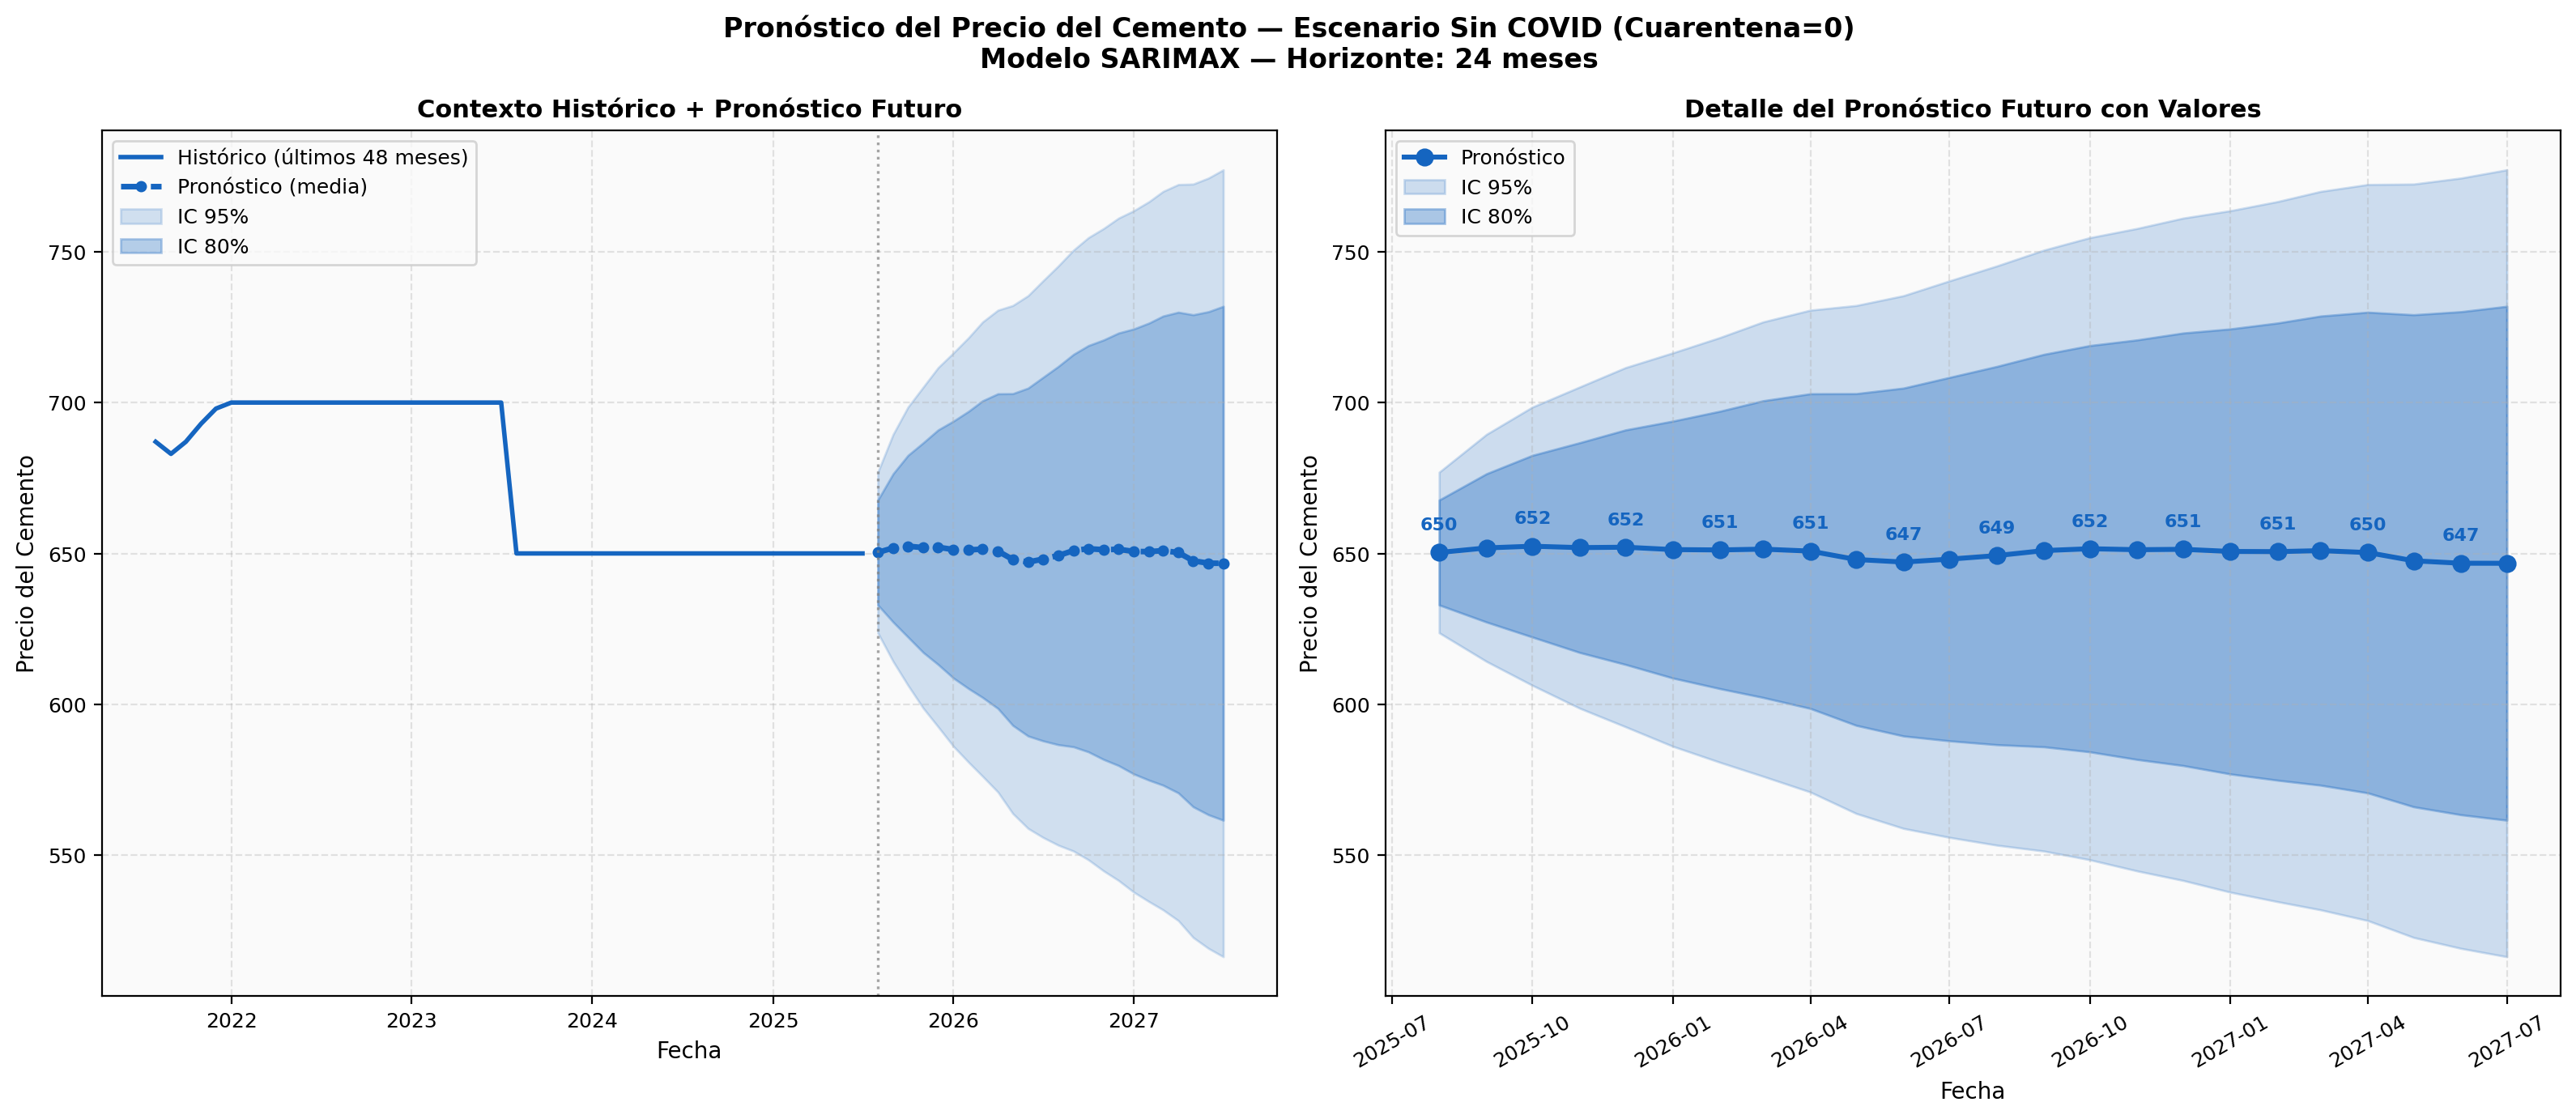
\includegraphics[width=\textwidth]{predicciones/prediccion_sarimax_ladrillo/graficos/12a_pronostico_sin_covid.png}
    \caption{Pronóstico SARIMAX del precio del ladrillo a 24 meses -- escenario sin efecto pandémico.}
    \label{fig:sarimax_ladrillo_sin_covid}
\end{figure}

\begin{figure}[ht]
    \centering
    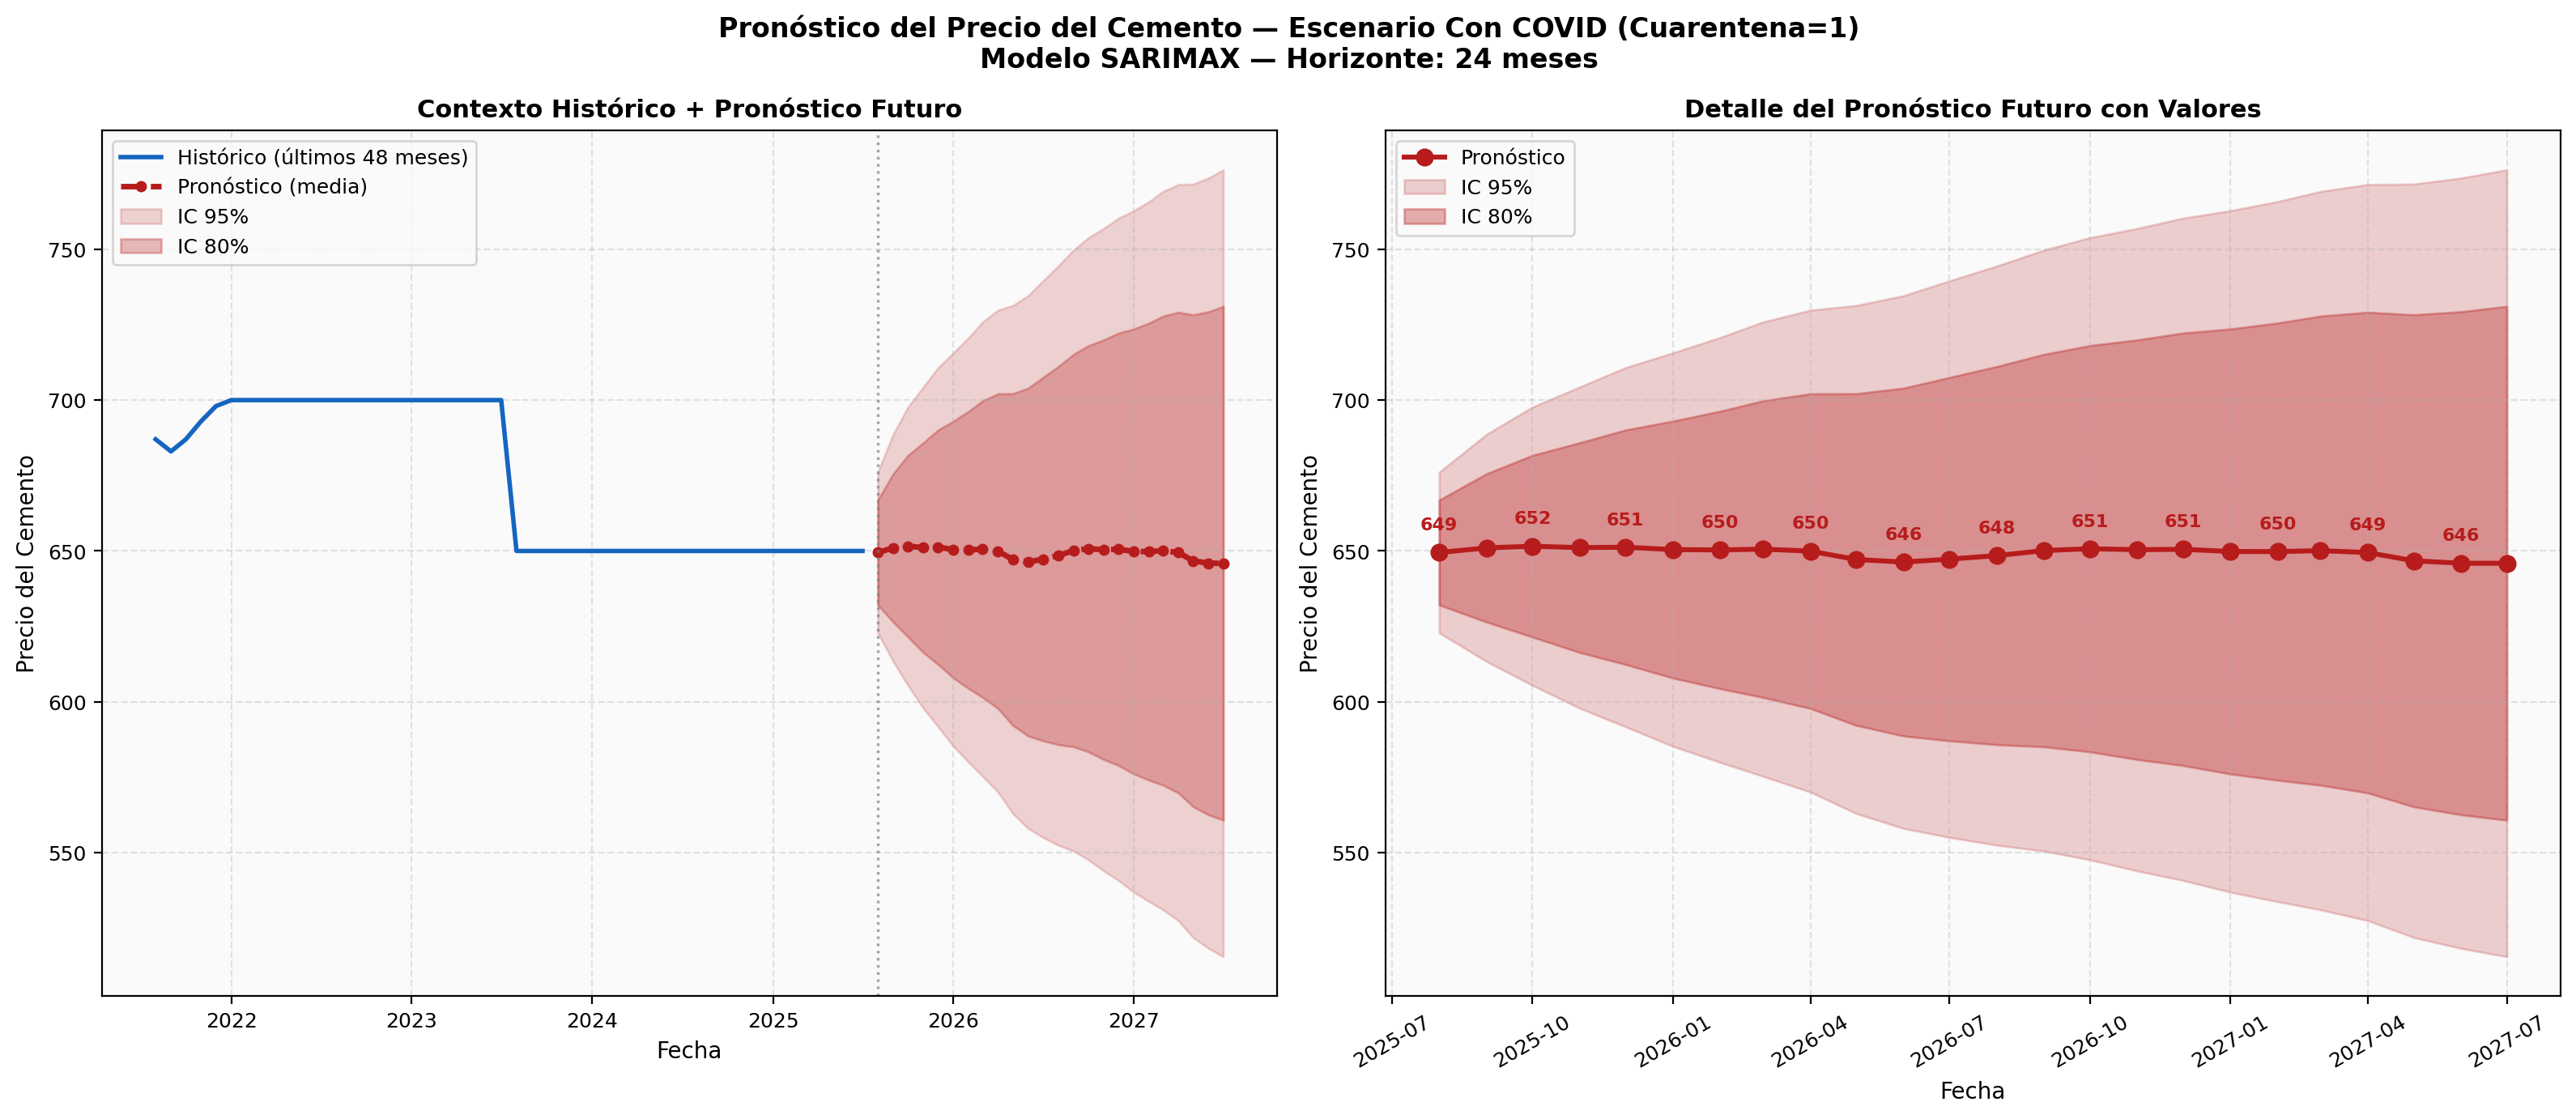
\includegraphics[width=\textwidth]{predicciones/prediccion_sarimax_ladrillo/graficos/12b_pronostico_con_covid.png}
    \caption{Pronóstico SARIMAX del precio del ladrillo a 24 meses -- escenario con efecto pandémico.}
    \label{fig:sarimax_ladrillo_con_covid}
\end{figure}

\justify
La diferencia entre ambos escenarios es de apenas Gs.~$-0{,}82$ por mes, un valor aún más reducido que el observado para el cemento (Gs.~$-23{,}48$) y completamente insignificante frente al nivel de precios de la serie (Gs.~650). Este resultado es coherente con el coeficiente estimado para la variable \texttt{Cuarentena} en el modelo SARIMAX del ladrillo ($-0{,}819$~Gs., $p=0{,}999$), que resultó estadísticamente no significativo. La insensibilidad del modelo SARIMAX ante el \textit{shock} pandémico se repite en ambos materiales de construcción, confirmando que la estructura lineal integrada del modelo ---capaz de capturar la tendencia general y la contribución hidrológica--- carece de la flexibilidad necesaria para representar los efectos no lineales y asimétricos de perturbaciones como la pandemia de COVID-19. Los modelos LSTM y GRU que se presentan en las secciones siguientes ofrecen un contraste instructivo al respecto.
